\documentclass[12pt, a4paper, twoside, openright]{ociamthesis}  % default square logo 



%load any additional packages

%%Pacchetti utili anche se non necessari
%\usepackage{amsfonts}
%\usepackage{amsmath}
%\usepackage{latexsym}
%\usepackage{tabularx}
\usepackage[english]{babel}
%\usepackage[hidelinks,bookmarks=true]{hyperref}
%\usepackage{graphicx}
%\usepackage{floatflt}
%\usepackage{float}
%%\usepackage[latin1]{inputenc} 
%\usepackage{multirow} 
%\usepackage[titletoc]{appendix}
%\usepackage{listings}
%\usepackage{xcolor}
%\usepackage{longtable} 
%\usepackage{verbatim}
%\usepackage{booktabs}
%\usepackage{amsmath,amssymb,amsfonts}
%\usepackage{nameref}
%\usepackage{longtable}
%\usepackage{lscape} 
%\usepackage{csquotes}
%\usepackage{listings}
%\usepackage[flushleft]{threeparttable}
%%\usepackage[caption = false]{subfig}
%\usepackage{slashbox}
%\usepackage{rotating}
%\usepackage{pdflscape}

\usepackage{lineno,hyperref}
\modulolinenumbers[5]
\usepackage{url}
\usepackage{times,amsmath,epsfig,amssymb}
\usepackage{subfigure}
\usepackage{wrapfig}
\usepackage{amsfonts}
%\usepackage{hyperref}
%\usepackage{cite}
\usepackage{ctable}
\usepackage{tabularx,booktabs}
\usepackage{amsmath}
\usepackage{svg}
\newtheorem{theorem}{Theorem}
\newtheorem{corollary}[theorem]{Corollary}
\newtheorem{definition}{Definition}
\newtheorem{example}{Example}
\newtheorem{lemma}[theorem]{Lemma}
\newtheorem{proposition}[theorem]{Proposition}
\newtheorem{problem}{Problem}
\newtheorem{remark}{Remark}
\newtheorem{assumption}{Assumption}

\newcommand{\X}{\mathcal{X}}
\newcommand{\Xd}{\mathcal{X}_d}
\newcommand{\Xdi}{\mathcal{X}_{d_\iota}}
\newcommand{\Xdj}{\mathcal{X}_{d_\jmath}}
\newcommand{\Xu}{\mathcal{X}_u}
\newcommand{\Y}{\mathcal{Y}}
\newcommand{\Yij}{\mathcal{Y}_{ij}}
\newcommand{\Real}{\mathbb{R}}
\newcommand{\Dij}{\mathcal{D}_{ij}}
\newcommand{\D}{\mathcal{D}}
\newcommand{\T}{\mathcal{T}}
\newcommand{\Tij}{\mathcal{T}_{ij}}
\newcommand{\Tilj}{\mathcal{T}_{i\ell_j}}
\newcommand{\F}{\mathcal{F}}
\newcommand{\Fij}{\mathcal{F}_{ij}}
\newcommand{\Filj}{\mathcal{F}_{i\ell_j}}
\usepackage{lineno,hyperref}
\modulolinenumbers[5]

\usepackage{setspace}
\DeclareMathOperator{\tr}{tr}
\def\BibTeX{{\rm B\kern-.05em{\sc i\kern-.025em b}\kern-.08em
    T\kern-.1667em\lower.7ex\hbox{E}\kern-.125emX}}

%Footnote without number

\newcommand\blfootnote[1]{%
  \begingroup
  \renewcommand\thefootnote{}\footnote{#1}%
  \addtocounter{footnote}{-1}%
  \endgroup
}
\usepackage[toc,page]{appendix}%per appendici
\usepackage{listings} %nuovo pacchetto
%Per Colori di PYTHON
\definecolor{mygreen}{rgb}{0,0.7,0}
\definecolor{mygray}{rgb}{0.5,0.5,0.5}
\definecolor{mymauve}{rgb}{0.58,0,0.82}
\definecolor{myred}{rgb}{0.8,0,0}
\definecolor{myorange}{rgb}{1,0.5,0}
\definecolor{mycyan}{rgb}{0.9,1,0.9}

\lstset{ %
  backgroundcolor=\color{white},   % choose the background color; you must add \usepackage{color} or \usepackage{xcolor}; should come as last argument
  basicstyle=\footnotesize,        % the size of the fonts that are used for the code
  breakatwhitespace=false,         % sets if automatic breaks should only happen at whitespace
  breaklines=true,                 % sets automatic line breaking
  captionpos=b,                    % sets the caption-position to bottom
  commentstyle=\color{myred},    % comment style
  deletekeywords={...},            % if you want to delete keywords from the given language
  escapeinside={\%*}{*)},          % if you want to add LaTeX within your code
  extendedchars=true,              % lets you use non-ASCII characters; for 8-bits encodings only, does not work with UTF-8
  frame=single,	                   % adds a frame around the code
  keepspaces=true,                 % keeps spaces in text, useful for keeping indentation of code (possibly needs columns=flexible)
  %keywordstyle=\color{myorange},       % keyword style
  %language=Octave,                 % the language of the code  
  morekeywords={import,from,class,def,for,while,if,is,in,elif,else,not,and,or,print,break,continue,return,access,as,del,except,exec,finally,global,import,lambda,pass,print,raise,try,assert},           % if you want to add more keywords to the set
  keywordstyle={\color{myorange}},
  morekeywords={[2] True,None,},
keywordstyle={[2]\color{mymauve}},
    emph=[1]{True,False,None,format,ord,len,str,},
    emphstyle=[1]{\color{mymauve}},  
	emph=[2]{import,from,class,def,for,while,if,is,in,elif,else,not,and,or,print,break,continue,return,access,as,del,except,exec,finally,global,import,lambda,pass,print,raise,try,assert,},
    emphstyle=[2]{\color{myorange}},  
emph=[3]{click_and_crop,},  
  emphstyle=[3]{\color{blue}},  
  numbers=left,                    % where to put the line-numbers; possible values are (none, left, right)
  numbersep=5pt,                   % how far the line-numbers are from the code
  numberstyle=\tiny\color{mygray},
  %firstnumber=3, % the style that is used for the line-numbers
  numberfirstline=true,  
  rulecolor=\color{black},         % if not set, the frame-color may be changed on line-breaks within not-black text (e.g. comments (green here))
  showspaces=false,                % show spaces everywhere adding particular underscores; it overrides 'showstringspaces'
  showstringspaces=false,          % underline spaces within strings only
  showtabs=false,                  % show tabs within strings adding particular underscores
  stepnumber=1,                    % the step between two line-numbers. If it's 1, each line will be numbered
  stringstyle=\color{mygreen},		% string literal style   
  tabsize=2,	                   % sets default tabsize to 2 spaces
  %title=\lstname                   % show the filename of files included with \lstinputlisting; also try caption instead of title %%%Decommentare per far vedere il nome del file sotto al codice
}

 %%%%%%%%%%%%%%%%%%%%%%%%%%%%%%%%%%%%%%%%%%%%%%%%%%%%%%%%%%%%%%%%%%%%%%%%%%%%%%%% 
%%% ~ Arduino Language - Arduino IDE Colors ~                                  %%%
%%%                                                                            %%%
%%% Kyle Rocha-Brownell | 10/2/2017 | No Licence                               %%%
%%% -------------------------------------------------------------------------- %%%
%%%                                                                            %%%
%%% Place this file in your working directory (next to the latex file you're   %%%
%%% working on).  To add it to your project, place:                            %%%
%%%     %%%%%%%%%%%%%%%%%%%%%%%%%%%%%%%%%%%%%%%%%%%%%%%%%%%%%%%%%%%%%%%%%%%%%%%%%%%%%%%% 
%%% ~ Arduino Language - Arduino IDE Colors ~                                  %%%
%%%                                                                            %%%
%%% Kyle Rocha-Brownell | 10/2/2017 | No Licence                               %%%
%%% -------------------------------------------------------------------------- %%%
%%%                                                                            %%%
%%% Place this file in your working directory (next to the latex file you're   %%%
%%% working on).  To add it to your project, place:                            %%%
%%%     %%%%%%%%%%%%%%%%%%%%%%%%%%%%%%%%%%%%%%%%%%%%%%%%%%%%%%%%%%%%%%%%%%%%%%%%%%%%%%%% 
%%% ~ Arduino Language - Arduino IDE Colors ~                                  %%%
%%%                                                                            %%%
%%% Kyle Rocha-Brownell | 10/2/2017 | No Licence                               %%%
%%% -------------------------------------------------------------------------- %%%
%%%                                                                            %%%
%%% Place this file in your working directory (next to the latex file you're   %%%
%%% working on).  To add it to your project, place:                            %%%
%%%    \input{arduinoLanguage.tex}                                             %%%
%%% somewhere before \begin{document} in your latex file.                      %%%
%%%                                                                            %%%
%%% In your document, place your arduino code between:                         %%%
%%%   \begin{lstlisting}[language=Arduino]                                     %%%
%%% and:                                                                       %%%
%%%   \end{lstlisting}                                                         %%%
%%%                                                                            %%%
%%% Or create your own style to add non-built-in functions and variables.      %%%
%%%                                                                            %%%
 %%%%%%%%%%%%%%%%%%%%%%%%%%%%%%%%%%%%%%%%%%%%%%%%%%%%%%%%%%%%%%%%%%%%%%%%%%%%%%%% 

\usepackage{color}
\usepackage{listings}    
\usepackage{courier}

%%% Define Custom IDE Colors %%%
\definecolor{arduinoGreen}    {rgb} {0.17, 0.43, 0.01}
\definecolor{arduinoGrey}     {rgb} {0.47, 0.47, 0.33}
\definecolor{arduinoOrange}   {rgb} {0.8 , 0.4 , 0   }
\definecolor{arduinoBlue}     {rgb} {0.01, 0.61, 0.98}
\definecolor{arduinoDarkBlue} {rgb} {0.0 , 0.2 , 0.5 }

%%% Define Arduino Language %%%
\lstdefinelanguage{Arduino}{
  language=C++, % begin with default C++ settings 
%
%
  %%% Keyword Color Group 1 %%%  (called KEYWORD3 by arduino)
  keywordstyle=\color{arduinoGreen},   
  deletekeywords={  % remove all arduino keywords that might be in c++
                break, case, override, final, continue, default, do, else, for, 
                if, return, goto, switch, throw, try, while, setup, loop, export, 
                not, or, and, xor, include, define, elif, else, error, if, ifdef, 
                ifndef, pragma, warning,
                HIGH, LOW, INPUT, INPUT_PULLUP, OUTPUT, DEC, BIN, HEX, OCT, PI, 
                HALF_PI, TWO_PI, LSBFIRST, MSBFIRST, CHANGE, FALLING, RISING, 
                DEFAULT, EXTERNAL, INTERNAL, INTERNAL1V1, INTERNAL2V56, LED_BUILTIN, 
                LED_BUILTIN_RX, LED_BUILTIN_TX, DIGITAL_MESSAGE, FIRMATA_STRING, 
                ANALOG_MESSAGE, REPORT_DIGITAL, REPORT_ANALOG, SET_PIN_MODE, 
                SYSTEM_RESET, SYSEX_START, auto, int8_t, int16_t, int32_t, int64_t, 
                uint8_t, uint16_t, uint32_t, uint64_t, char16_t, char32_t, operator, 
                enum, delete, bool, boolean, byte, char, const, false, float, double, 
                null, NULL, int, long, new, private, protected, public, short, 
                signed, static, volatile, String, void, true, unsigned, word, array, 
                sizeof, dynamic_cast, typedef, const_cast, struct, static_cast, union, 
                friend, extern, class, reinterpret_cast, register, explicit, inline, 
                _Bool, complex, _Complex, _Imaginary, atomic_bool, atomic_char, 
                atomic_schar, atomic_uchar, atomic_short, atomic_ushort, atomic_int, 
                atomic_uint, atomic_long, atomic_ulong, atomic_llong, atomic_ullong, 
                virtual, PROGMEM,
                Serial, Serial1, Serial2, Serial3, SerialUSB, Keyboard, Mouse,
                abs, acos, asin, atan, atan2, ceil, constrain, cos, degrees, exp, 
                floor, log, map, max, min, radians, random, randomSeed, round, sin, 
                sq, sqrt, tan, pow, bitRead, bitWrite, bitSet, bitClear, bit, 
                highByte, lowByte, analogReference, analogRead, 
                analogReadResolution, analogWrite, analogWriteResolution, 
                attachInterrupt, detachInterrupt, digitalPinToInterrupt, delay, 
                delayMicroseconds, digitalWrite, digitalRead, interrupts, millis, 
                micros, noInterrupts, noTone, pinMode, pulseIn, pulseInLong, shiftIn, 
                shiftOut, tone, yield, Stream, begin, end, peek, read, print, 
                println, available, availableForWrite, flush, setTimeout, find, 
                findUntil, parseInt, parseFloat, readBytes, readBytesUntil, readString, 
                readStringUntil, trim, toUpperCase, toLowerCase, charAt, compareTo, 
                concat, endsWith, startsWith, equals, equalsIgnoreCase, getBytes, 
                indexOf, lastIndexOf, length, replace, setCharAt, substring, 
                toCharArray, toInt, press, release, releaseAll, accept, click, move, 
                isPressed, isAlphaNumeric, isAlpha, isAscii, isWhitespace, isControl, 
                isDigit, isGraph, isLowerCase, isPrintable, isPunct, isSpace, 
                isUpperCase, isHexadecimalDigit, 
                }, 
  morekeywords={   % add arduino structures to group 1
                break, case, override, final, continue, default, do, else, for, 
                if, return, goto, switch, throw, try, while, setup, loop, export, 
                not, or, and, xor, include, define, elif, else, error, if, ifdef, 
                ifndef, pragma, warning,
                }, 
% 
%
  %%% Keyword Color Group 2 %%%  (called LITERAL1 by arduino)
  keywordstyle=[2]\color{arduinoBlue},   
  keywords=[2]{   % add variables and dataTypes as 2nd group  
                HIGH, LOW, INPUT, INPUT_PULLUP, OUTPUT, DEC, BIN, HEX, OCT, PI, 
                HALF_PI, TWO_PI, LSBFIRST, MSBFIRST, CHANGE, FALLING, RISING, 
                DEFAULT, EXTERNAL, INTERNAL, INTERNAL1V1, INTERNAL2V56, LED_BUILTIN, 
                LED_BUILTIN_RX, LED_BUILTIN_TX, DIGITAL_MESSAGE, FIRMATA_STRING, 
                ANALOG_MESSAGE, REPORT_DIGITAL, REPORT_ANALOG, SET_PIN_MODE, 
                SYSTEM_RESET, SYSEX_START, auto, int8_t, int16_t, int32_t, int64_t, 
                uint8_t, uint16_t, uint32_t, uint64_t, char16_t, char32_t, operator, 
                enum, delete, bool, boolean, byte, char, const, false, float, double, 
                null, NULL, int, long, new, private, protected, public, short, 
                signed, static, volatile, String, void, true, unsigned, word, array, 
                sizeof, dynamic_cast, typedef, const_cast, struct, static_cast, union, 
                friend, extern, class, reinterpret_cast, register, explicit, inline, 
                _Bool, complex, _Complex, _Imaginary, atomic_bool, atomic_char, 
                atomic_schar, atomic_uchar, atomic_short, atomic_ushort, atomic_int, 
                atomic_uint, atomic_long, atomic_ulong, atomic_llong, atomic_ullong, 
                virtual, PROGMEM,
                },  
% 
%
  %%% Keyword Color Group 3 %%%  (called KEYWORD1 by arduino)
  keywordstyle=[3]\bfseries\color{arduinoOrange},
  keywords=[3]{  % add built-in functions as a 3rd group
                Serial, Serial1, Serial2, Serial3, SerialUSB, Keyboard, Mouse,
                },      
%
%
  %%% Keyword Color Group 4 %%%  (called KEYWORD2 by arduino)
  keywordstyle=[4]\color{arduinoOrange},
  keywords=[4]{  % add more built-in functions as a 4th group
                abs, acos, asin, atan, atan2, ceil, constrain, cos, degrees, exp, 
                floor, log, map, max, min, radians, random, randomSeed, round, sin, 
                sq, sqrt, tan, pow, bitRead, bitWrite, bitSet, bitClear, bit, 
                highByte, lowByte, analogReference, analogRead, 
                analogReadResolution, analogWrite, analogWriteResolution, 
                attachInterrupt, detachInterrupt, digitalPinToInterrupt, delay, 
                delayMicroseconds, digitalWrite, digitalRead, interrupts, millis, 
                micros, noInterrupts, noTone, pinMode, pulseIn, pulseInLong, shiftIn, 
                shiftOut, tone, yield, Stream, begin, end, peek, read, print, 
                println, available, availableForWrite, flush, setTimeout, find, 
                findUntil, parseInt, parseFloat, readBytes, readBytesUntil, readString, 
                readStringUntil, trim, toUpperCase, toLowerCase, charAt, compareTo, 
                concat, endsWith, startsWith, equals, equalsIgnoreCase, getBytes, 
                indexOf, lastIndexOf, length, replace, setCharAt, substring, 
                toCharArray, toInt, press, release, releaseAll, accept, click, move, 
                isPressed, isAlphaNumeric, isAlpha, isAscii, isWhitespace, isControl, 
                isDigit, isGraph, isLowerCase, isPrintable, isPunct, isSpace, 
                isUpperCase, isHexadecimalDigit, 
                },      
%
%
  %%% Set Other Colors %%%
  stringstyle=\color{arduinoDarkBlue},    
  commentstyle=\color{arduinoGrey},    
%          
%   
  %%%% Line Numbering %%%%
  numbers=left,                    
  numbersep=5pt,                   
  numberstyle=\color{arduinoGrey},    
  %stepnumber=2,                      % show every 2 line numbers
%
%
  %%%% Code Box Style %%%%
  breaklines=true,                    % wordwrapping
  tabsize=2,         
  basicstyle=\ttfamily  
}
                                             %%%
%%% somewhere before \begin{document} in your latex file.                      %%%
%%%                                                                            %%%
%%% In your document, place your arduino code between:                         %%%
%%%   \begin{lstlisting}[language=Arduino]                                     %%%
%%% and:                                                                       %%%
%%%   \end{lstlisting}                                                         %%%
%%%                                                                            %%%
%%% Or create your own style to add non-built-in functions and variables.      %%%
%%%                                                                            %%%
 %%%%%%%%%%%%%%%%%%%%%%%%%%%%%%%%%%%%%%%%%%%%%%%%%%%%%%%%%%%%%%%%%%%%%%%%%%%%%%%% 

\usepackage{color}
\usepackage{listings}    
\usepackage{courier}

%%% Define Custom IDE Colors %%%
\definecolor{arduinoGreen}    {rgb} {0.17, 0.43, 0.01}
\definecolor{arduinoGrey}     {rgb} {0.47, 0.47, 0.33}
\definecolor{arduinoOrange}   {rgb} {0.8 , 0.4 , 0   }
\definecolor{arduinoBlue}     {rgb} {0.01, 0.61, 0.98}
\definecolor{arduinoDarkBlue} {rgb} {0.0 , 0.2 , 0.5 }

%%% Define Arduino Language %%%
\lstdefinelanguage{Arduino}{
  language=C++, % begin with default C++ settings 
%
%
  %%% Keyword Color Group 1 %%%  (called KEYWORD3 by arduino)
  keywordstyle=\color{arduinoGreen},   
  deletekeywords={  % remove all arduino keywords that might be in c++
                break, case, override, final, continue, default, do, else, for, 
                if, return, goto, switch, throw, try, while, setup, loop, export, 
                not, or, and, xor, include, define, elif, else, error, if, ifdef, 
                ifndef, pragma, warning,
                HIGH, LOW, INPUT, INPUT_PULLUP, OUTPUT, DEC, BIN, HEX, OCT, PI, 
                HALF_PI, TWO_PI, LSBFIRST, MSBFIRST, CHANGE, FALLING, RISING, 
                DEFAULT, EXTERNAL, INTERNAL, INTERNAL1V1, INTERNAL2V56, LED_BUILTIN, 
                LED_BUILTIN_RX, LED_BUILTIN_TX, DIGITAL_MESSAGE, FIRMATA_STRING, 
                ANALOG_MESSAGE, REPORT_DIGITAL, REPORT_ANALOG, SET_PIN_MODE, 
                SYSTEM_RESET, SYSEX_START, auto, int8_t, int16_t, int32_t, int64_t, 
                uint8_t, uint16_t, uint32_t, uint64_t, char16_t, char32_t, operator, 
                enum, delete, bool, boolean, byte, char, const, false, float, double, 
                null, NULL, int, long, new, private, protected, public, short, 
                signed, static, volatile, String, void, true, unsigned, word, array, 
                sizeof, dynamic_cast, typedef, const_cast, struct, static_cast, union, 
                friend, extern, class, reinterpret_cast, register, explicit, inline, 
                _Bool, complex, _Complex, _Imaginary, atomic_bool, atomic_char, 
                atomic_schar, atomic_uchar, atomic_short, atomic_ushort, atomic_int, 
                atomic_uint, atomic_long, atomic_ulong, atomic_llong, atomic_ullong, 
                virtual, PROGMEM,
                Serial, Serial1, Serial2, Serial3, SerialUSB, Keyboard, Mouse,
                abs, acos, asin, atan, atan2, ceil, constrain, cos, degrees, exp, 
                floor, log, map, max, min, radians, random, randomSeed, round, sin, 
                sq, sqrt, tan, pow, bitRead, bitWrite, bitSet, bitClear, bit, 
                highByte, lowByte, analogReference, analogRead, 
                analogReadResolution, analogWrite, analogWriteResolution, 
                attachInterrupt, detachInterrupt, digitalPinToInterrupt, delay, 
                delayMicroseconds, digitalWrite, digitalRead, interrupts, millis, 
                micros, noInterrupts, noTone, pinMode, pulseIn, pulseInLong, shiftIn, 
                shiftOut, tone, yield, Stream, begin, end, peek, read, print, 
                println, available, availableForWrite, flush, setTimeout, find, 
                findUntil, parseInt, parseFloat, readBytes, readBytesUntil, readString, 
                readStringUntil, trim, toUpperCase, toLowerCase, charAt, compareTo, 
                concat, endsWith, startsWith, equals, equalsIgnoreCase, getBytes, 
                indexOf, lastIndexOf, length, replace, setCharAt, substring, 
                toCharArray, toInt, press, release, releaseAll, accept, click, move, 
                isPressed, isAlphaNumeric, isAlpha, isAscii, isWhitespace, isControl, 
                isDigit, isGraph, isLowerCase, isPrintable, isPunct, isSpace, 
                isUpperCase, isHexadecimalDigit, 
                }, 
  morekeywords={   % add arduino structures to group 1
                break, case, override, final, continue, default, do, else, for, 
                if, return, goto, switch, throw, try, while, setup, loop, export, 
                not, or, and, xor, include, define, elif, else, error, if, ifdef, 
                ifndef, pragma, warning,
                }, 
% 
%
  %%% Keyword Color Group 2 %%%  (called LITERAL1 by arduino)
  keywordstyle=[2]\color{arduinoBlue},   
  keywords=[2]{   % add variables and dataTypes as 2nd group  
                HIGH, LOW, INPUT, INPUT_PULLUP, OUTPUT, DEC, BIN, HEX, OCT, PI, 
                HALF_PI, TWO_PI, LSBFIRST, MSBFIRST, CHANGE, FALLING, RISING, 
                DEFAULT, EXTERNAL, INTERNAL, INTERNAL1V1, INTERNAL2V56, LED_BUILTIN, 
                LED_BUILTIN_RX, LED_BUILTIN_TX, DIGITAL_MESSAGE, FIRMATA_STRING, 
                ANALOG_MESSAGE, REPORT_DIGITAL, REPORT_ANALOG, SET_PIN_MODE, 
                SYSTEM_RESET, SYSEX_START, auto, int8_t, int16_t, int32_t, int64_t, 
                uint8_t, uint16_t, uint32_t, uint64_t, char16_t, char32_t, operator, 
                enum, delete, bool, boolean, byte, char, const, false, float, double, 
                null, NULL, int, long, new, private, protected, public, short, 
                signed, static, volatile, String, void, true, unsigned, word, array, 
                sizeof, dynamic_cast, typedef, const_cast, struct, static_cast, union, 
                friend, extern, class, reinterpret_cast, register, explicit, inline, 
                _Bool, complex, _Complex, _Imaginary, atomic_bool, atomic_char, 
                atomic_schar, atomic_uchar, atomic_short, atomic_ushort, atomic_int, 
                atomic_uint, atomic_long, atomic_ulong, atomic_llong, atomic_ullong, 
                virtual, PROGMEM,
                },  
% 
%
  %%% Keyword Color Group 3 %%%  (called KEYWORD1 by arduino)
  keywordstyle=[3]\bfseries\color{arduinoOrange},
  keywords=[3]{  % add built-in functions as a 3rd group
                Serial, Serial1, Serial2, Serial3, SerialUSB, Keyboard, Mouse,
                },      
%
%
  %%% Keyword Color Group 4 %%%  (called KEYWORD2 by arduino)
  keywordstyle=[4]\color{arduinoOrange},
  keywords=[4]{  % add more built-in functions as a 4th group
                abs, acos, asin, atan, atan2, ceil, constrain, cos, degrees, exp, 
                floor, log, map, max, min, radians, random, randomSeed, round, sin, 
                sq, sqrt, tan, pow, bitRead, bitWrite, bitSet, bitClear, bit, 
                highByte, lowByte, analogReference, analogRead, 
                analogReadResolution, analogWrite, analogWriteResolution, 
                attachInterrupt, detachInterrupt, digitalPinToInterrupt, delay, 
                delayMicroseconds, digitalWrite, digitalRead, interrupts, millis, 
                micros, noInterrupts, noTone, pinMode, pulseIn, pulseInLong, shiftIn, 
                shiftOut, tone, yield, Stream, begin, end, peek, read, print, 
                println, available, availableForWrite, flush, setTimeout, find, 
                findUntil, parseInt, parseFloat, readBytes, readBytesUntil, readString, 
                readStringUntil, trim, toUpperCase, toLowerCase, charAt, compareTo, 
                concat, endsWith, startsWith, equals, equalsIgnoreCase, getBytes, 
                indexOf, lastIndexOf, length, replace, setCharAt, substring, 
                toCharArray, toInt, press, release, releaseAll, accept, click, move, 
                isPressed, isAlphaNumeric, isAlpha, isAscii, isWhitespace, isControl, 
                isDigit, isGraph, isLowerCase, isPrintable, isPunct, isSpace, 
                isUpperCase, isHexadecimalDigit, 
                },      
%
%
  %%% Set Other Colors %%%
  stringstyle=\color{arduinoDarkBlue},    
  commentstyle=\color{arduinoGrey},    
%          
%   
  %%%% Line Numbering %%%%
  numbers=left,                    
  numbersep=5pt,                   
  numberstyle=\color{arduinoGrey},    
  %stepnumber=2,                      % show every 2 line numbers
%
%
  %%%% Code Box Style %%%%
  breaklines=true,                    % wordwrapping
  tabsize=2,         
  basicstyle=\ttfamily  
}
                                             %%%
%%% somewhere before \begin{document} in your latex file.                      %%%
%%%                                                                            %%%
%%% In your document, place your arduino code between:                         %%%
%%%   \begin{lstlisting}[language=Arduino]                                     %%%
%%% and:                                                                       %%%
%%%   \end{lstlisting}                                                         %%%
%%%                                                                            %%%
%%% Or create your own style to add non-built-in functions and variables.      %%%
%%%                                                                            %%%
 %%%%%%%%%%%%%%%%%%%%%%%%%%%%%%%%%%%%%%%%%%%%%%%%%%%%%%%%%%%%%%%%%%%%%%%%%%%%%%%% 

\usepackage{color}
\usepackage{listings}    
\usepackage{courier}

%%% Define Custom IDE Colors %%%
\definecolor{arduinoGreen}    {rgb} {0.17, 0.43, 0.01}
\definecolor{arduinoGrey}     {rgb} {0.47, 0.47, 0.33}
\definecolor{arduinoOrange}   {rgb} {0.8 , 0.4 , 0   }
\definecolor{arduinoBlue}     {rgb} {0.01, 0.61, 0.98}
\definecolor{arduinoDarkBlue} {rgb} {0.0 , 0.2 , 0.5 }

%%% Define Arduino Language %%%
\lstdefinelanguage{Arduino}{
  language=C++, % begin with default C++ settings 
%
%
  %%% Keyword Color Group 1 %%%  (called KEYWORD3 by arduino)
  keywordstyle=\color{arduinoGreen},   
  deletekeywords={  % remove all arduino keywords that might be in c++
                break, case, override, final, continue, default, do, else, for, 
                if, return, goto, switch, throw, try, while, setup, loop, export, 
                not, or, and, xor, include, define, elif, else, error, if, ifdef, 
                ifndef, pragma, warning,
                HIGH, LOW, INPUT, INPUT_PULLUP, OUTPUT, DEC, BIN, HEX, OCT, PI, 
                HALF_PI, TWO_PI, LSBFIRST, MSBFIRST, CHANGE, FALLING, RISING, 
                DEFAULT, EXTERNAL, INTERNAL, INTERNAL1V1, INTERNAL2V56, LED_BUILTIN, 
                LED_BUILTIN_RX, LED_BUILTIN_TX, DIGITAL_MESSAGE, FIRMATA_STRING, 
                ANALOG_MESSAGE, REPORT_DIGITAL, REPORT_ANALOG, SET_PIN_MODE, 
                SYSTEM_RESET, SYSEX_START, auto, int8_t, int16_t, int32_t, int64_t, 
                uint8_t, uint16_t, uint32_t, uint64_t, char16_t, char32_t, operator, 
                enum, delete, bool, boolean, byte, char, const, false, float, double, 
                null, NULL, int, long, new, private, protected, public, short, 
                signed, static, volatile, String, void, true, unsigned, word, array, 
                sizeof, dynamic_cast, typedef, const_cast, struct, static_cast, union, 
                friend, extern, class, reinterpret_cast, register, explicit, inline, 
                _Bool, complex, _Complex, _Imaginary, atomic_bool, atomic_char, 
                atomic_schar, atomic_uchar, atomic_short, atomic_ushort, atomic_int, 
                atomic_uint, atomic_long, atomic_ulong, atomic_llong, atomic_ullong, 
                virtual, PROGMEM,
                Serial, Serial1, Serial2, Serial3, SerialUSB, Keyboard, Mouse,
                abs, acos, asin, atan, atan2, ceil, constrain, cos, degrees, exp, 
                floor, log, map, max, min, radians, random, randomSeed, round, sin, 
                sq, sqrt, tan, pow, bitRead, bitWrite, bitSet, bitClear, bit, 
                highByte, lowByte, analogReference, analogRead, 
                analogReadResolution, analogWrite, analogWriteResolution, 
                attachInterrupt, detachInterrupt, digitalPinToInterrupt, delay, 
                delayMicroseconds, digitalWrite, digitalRead, interrupts, millis, 
                micros, noInterrupts, noTone, pinMode, pulseIn, pulseInLong, shiftIn, 
                shiftOut, tone, yield, Stream, begin, end, peek, read, print, 
                println, available, availableForWrite, flush, setTimeout, find, 
                findUntil, parseInt, parseFloat, readBytes, readBytesUntil, readString, 
                readStringUntil, trim, toUpperCase, toLowerCase, charAt, compareTo, 
                concat, endsWith, startsWith, equals, equalsIgnoreCase, getBytes, 
                indexOf, lastIndexOf, length, replace, setCharAt, substring, 
                toCharArray, toInt, press, release, releaseAll, accept, click, move, 
                isPressed, isAlphaNumeric, isAlpha, isAscii, isWhitespace, isControl, 
                isDigit, isGraph, isLowerCase, isPrintable, isPunct, isSpace, 
                isUpperCase, isHexadecimalDigit, 
                }, 
  morekeywords={   % add arduino structures to group 1
                break, case, override, final, continue, default, do, else, for, 
                if, return, goto, switch, throw, try, while, setup, loop, export, 
                not, or, and, xor, include, define, elif, else, error, if, ifdef, 
                ifndef, pragma, warning,
                }, 
% 
%
  %%% Keyword Color Group 2 %%%  (called LITERAL1 by arduino)
  keywordstyle=[2]\color{arduinoBlue},   
  keywords=[2]{   % add variables and dataTypes as 2nd group  
                HIGH, LOW, INPUT, INPUT_PULLUP, OUTPUT, DEC, BIN, HEX, OCT, PI, 
                HALF_PI, TWO_PI, LSBFIRST, MSBFIRST, CHANGE, FALLING, RISING, 
                DEFAULT, EXTERNAL, INTERNAL, INTERNAL1V1, INTERNAL2V56, LED_BUILTIN, 
                LED_BUILTIN_RX, LED_BUILTIN_TX, DIGITAL_MESSAGE, FIRMATA_STRING, 
                ANALOG_MESSAGE, REPORT_DIGITAL, REPORT_ANALOG, SET_PIN_MODE, 
                SYSTEM_RESET, SYSEX_START, auto, int8_t, int16_t, int32_t, int64_t, 
                uint8_t, uint16_t, uint32_t, uint64_t, char16_t, char32_t, operator, 
                enum, delete, bool, boolean, byte, char, const, false, float, double, 
                null, NULL, int, long, new, private, protected, public, short, 
                signed, static, volatile, String, void, true, unsigned, word, array, 
                sizeof, dynamic_cast, typedef, const_cast, struct, static_cast, union, 
                friend, extern, class, reinterpret_cast, register, explicit, inline, 
                _Bool, complex, _Complex, _Imaginary, atomic_bool, atomic_char, 
                atomic_schar, atomic_uchar, atomic_short, atomic_ushort, atomic_int, 
                atomic_uint, atomic_long, atomic_ulong, atomic_llong, atomic_ullong, 
                virtual, PROGMEM,
                },  
% 
%
  %%% Keyword Color Group 3 %%%  (called KEYWORD1 by arduino)
  keywordstyle=[3]\bfseries\color{arduinoOrange},
  keywords=[3]{  % add built-in functions as a 3rd group
                Serial, Serial1, Serial2, Serial3, SerialUSB, Keyboard, Mouse,
                },      
%
%
  %%% Keyword Color Group 4 %%%  (called KEYWORD2 by arduino)
  keywordstyle=[4]\color{arduinoOrange},
  keywords=[4]{  % add more built-in functions as a 4th group
                abs, acos, asin, atan, atan2, ceil, constrain, cos, degrees, exp, 
                floor, log, map, max, min, radians, random, randomSeed, round, sin, 
                sq, sqrt, tan, pow, bitRead, bitWrite, bitSet, bitClear, bit, 
                highByte, lowByte, analogReference, analogRead, 
                analogReadResolution, analogWrite, analogWriteResolution, 
                attachInterrupt, detachInterrupt, digitalPinToInterrupt, delay, 
                delayMicroseconds, digitalWrite, digitalRead, interrupts, millis, 
                micros, noInterrupts, noTone, pinMode, pulseIn, pulseInLong, shiftIn, 
                shiftOut, tone, yield, Stream, begin, end, peek, read, print, 
                println, available, availableForWrite, flush, setTimeout, find, 
                findUntil, parseInt, parseFloat, readBytes, readBytesUntil, readString, 
                readStringUntil, trim, toUpperCase, toLowerCase, charAt, compareTo, 
                concat, endsWith, startsWith, equals, equalsIgnoreCase, getBytes, 
                indexOf, lastIndexOf, length, replace, setCharAt, substring, 
                toCharArray, toInt, press, release, releaseAll, accept, click, move, 
                isPressed, isAlphaNumeric, isAlpha, isAscii, isWhitespace, isControl, 
                isDigit, isGraph, isLowerCase, isPrintable, isPunct, isSpace, 
                isUpperCase, isHexadecimalDigit, 
                },      
%
%
  %%% Set Other Colors %%%
  stringstyle=\color{arduinoDarkBlue},    
  commentstyle=\color{arduinoGrey},    
%          
%   
  %%%% Line Numbering %%%%
  numbers=left,                    
  numbersep=5pt,                   
  numberstyle=\color{arduinoGrey},    
  %stepnumber=2,                      % show every 2 line numbers
%
%
  %%%% Code Box Style %%%%
  breaklines=true,                    % wordwrapping
  tabsize=2,         
  basicstyle=\ttfamily  
}
 
\lstdefinestyle{myArduino}{
  language=Arduino,
  %% Add other words needing highlighting below %%
  morekeywords=[1]{},                  % [1] -> dark green
  morekeywords=[2]{FILE_WRITE},        % [2] -> light blue
  morekeywords=[3]{SD, File},          % [3] -> bold orange
  morekeywords=[4]{open, exists},      % [4] -> orange
  %% The lines below add a nifty box around the code %%
  frame=shadowbox,
  rulesepcolor=\color{arduinoBlue},
}
%\usepackage[round]{natbib} 
%\usepackage{bibtopic}
%\newcommand*{\bibref}[1]{\citealt{#1}} %cite item

%% For Theorems, Lemmas, Definitions etc.   
%\usepackage{blindtext}
%\usepackage{amssymb}
%
%\usepackage{algorithm}
%\usepackage[noend]{algpseudocode}
%
%\usepackage{amsthm}
%
%\allowdisplaybreaks[1] 

%\newtheorem{theorem}{Theorem}
%\newtheorem{theorem}{Theorem}[section]
%\newtheorem{corollary}{Corollary}[theorem]
%\newtheorem{lemma}[theorem]{Lemma}

%\theoremstyle{remark}
%\newtheorem*{remark}{Remark}
%
%\theoremstyle{definition}
%\newtheorem{definition}{Definition}[section]

%\renewcommand\qedsymbol{$\blacksquare$}
%\newcommand {\ps} {\,{\bf \cdot}} % prodotto scalare
%
%\renewcommand{\mkbegdispquote}[2]{\itshape}
%
%\setcounter{MaxMatrixCols}{15}

%%%%%%%%%%%%%%%%%%%%%%%%%%%%%%%%%%%%%%%%%%%%%%%%

%\usepackage{titlesec}
%
%\titleclass{\subsubsubsection}{straight}[\subsection]
%
%\newcounter{subsubsubsection}[subsubsection]
%\renewcommand\thesubsubsubsection{\thesubsubsection.\arabic{subsubsubsection}}
%\renewcommand\theparagraph{\thesubsubsubsection.\arabic{paragraph}} % optional; useful if paragraphs are to be numbered
%
%\titleformat{\subsubsubsection}
%  {\normalfont\normalsize\bfseries}{\thesubsubsubsection}{1em}{}
%\titlespacing*{\subsubsubsection}
%{0pt}{3.25ex plus 1ex minus .2ex}{1.5ex plus .2ex}
%
%\makeatletter
%\renewcommand\paragraph{\@startsection{paragraph}{5}{\z@}%
%  {3.25ex \@plus1ex \@minus.2ex}%
%  {-1em}%
%  {\normalfont\normalsize\bfseries}}
%\renewcommand\subparagraph{\@startsection{subparagraph}{6}{\parindent}%
%  {3.25ex \@plus1ex \@minus .2ex}%
%  {-1em}%
%  {\normalfont\normalsize\bfseries}}
%\def\toclevel@subsubsubsection{4}
%\def\toclevel@paragraph{5}
%\def\toclevel@paragraph{6}
%\def\l@subsubsubsection{\@dottedtocline{4}{7em}{4em}}
%\def\l@paragraph{\@dottedtocline{5}{10em}{5em}}
%\def\l@subparagraph{\@dottedtocline{6}{14em}{6em}}
%\makeatother
%
%\setcounter{secnumdepth}{4}
%\setcounter{tocdepth}{4}
%
%\lstset { %
%    language=C++,
%    backgroundcolor=\color{black!5}, % set backgroundcolor
%    basicstyle=\footnotesize,% basic font setting
%}

%%%%%%%%%%%%%%%%%%%%%%%%%%%%%%%%%%%%%%%%%%%%%%%%%%%%%%%%%

%input macros (i.e. write your own macros file called mymacros.tex 
%and uncomment the next line)
%\include{mymacros}

\title{Model Identification and Control of Priority Queueing in Software Defined Networks} %\\[1ex] %your thesis title,
%}   %note \\[1ex] is a line break in the title

\author{Enrico Reticcioli}             %your name
\college{Universit\`a degli Studi dell'Aquila}  %your college

\advisor{Prof. Alessandro D'Innocenzo}
\coadvisor{Prof. Fabio Graziosi}
\coordinator{Prof. Vittorio Cortellessa}

\renewcommand{\submittedtext}{A thesis submitted for the degree of}
\degree{Doctor of Philosophy}     %the degree
\degreedate{2021}         %the degree date

%end the preamble and start the document
\begin{document}

%this baselineskip gives sufficient line spacing for an examiner to easily
%markup the thesis with comments
\baselineskip=18pt plus1pt

%set the number of sectioning levels that get number and appear in the contents
\setcounter{secnumdepth}{4}
\setcounter{tocdepth}{4}

\maketitle                  % create a title page from the preamble info
%\afterpage{\null\newpage}

%DA SCOMMENTARE PER LA STAMPA

%\begin{dedication}

\end{dedication}        % include a dedication.tex file
\begin{acknowledgements}

This work was supported by the Italian Government under Cipe resolution n.135 (Dec. 21, 2012), project \emph{INnovating City Planning through Information and Communication Technologies} (INCIPICT).

\end{acknowledgements}   % include an acknowledgements.tex file

%\afterpage{\null\newpage}
\addcontentsline{toc}{chapter}{Abstract}
\begin{abstract}
The heterogeneity of modern network infrastructures involves different devices and protocols bringing out several issues in organizing and optimizing network resources, making their coexistence a very challenging engineering problem. In this scenario, Software Defined Network (SDN) architectures decouple control and forwarding functionalities by enabling the network devices to be remotely configurable/programmable in run-time by a controller, and the underlying infrastructure to be abstracted from the application layer and the network services, with the final aim of increasing flexibility and performance. As a direct consequence identifying an accurate model of a network and forwarding devices is crucial in order to apply advanced control techniques such as Model Predictive Control (MPC) to optimize the network performance. An enabling factor in this direction is given by recent results that appropriately combine System Identification and Machine Learning techniques to obtain predictive models using historical data retrieved from a network. This paper presents a novel methodology to learn, starting from historical data and appropriately combining autoregressive exogenous(ARX) identification with Regression Trees and Random Forests, an accurate model of the dynamical input-output behavior of a network device that can be directly and efficiently used to optimally and dynamically control the bandwidth of the queues of switch ports, within the SDN paradigm. Both the Mininet network emulator environment and a real dataset obtained from measurements of the network of an Italian internet service provider (Sonicatel S.r.l.). have been used to validate the prediction accuracy of the derived predictive models. The benefits of the proposed dynamic queueing control methodology in terms of Packet Losses reduction and Bandwidth savings (i.e. improvement of the Quality of Service) has been finally demonstrated.
\end{abstract}          % include the abstract

\begin{romanpages}          % start roman page numbering
\tableofcontents            % generate and include a table of contents
\listoffigures              % generate and include a list of figures
\listoftables               % generate and include a list of figures
\end{romanpages}            % end roman page numbering

%\chapter*{\centering Notation}  

This is a list of notation I used in this work. In general, italic latin or greek letters denote sets and matrices, italic overline latin letters indicate vectors. Small subscripts latin or greek letters denote elements of sets, vectors, matrices, variables, functions, parameters, or indices. Due to a limited supply of alphabetical symbols, I have reused some for several purposes. Their usage should be clear form the context, nevertheless I apologize for any confusion that may arise. 
The following table summarizes the most commonly used symbols.
%
\begin{center}
\small
\begin{longtable}{ll}% p{1.4in}
\hline
 \textbf{Notation}   & \textbf{Explanation} \\ \hline
 \endhead
 \hline
 \endfoot
    SW                                      & Software \\
    HW                                      & Hardware \\
    HPV                                     & Hypervisor \\
    MC                                      & Mixed-Criticality \\
    MCES                                    & Mixed-Criticality Embedded Systems \\
    HMPS                                   & Heterogeneous Multi-Processor Systems \\
    H-MPSoC                                & Heterogeneous Multi-Processor System-On-Chip \\
    TDMA                                    & Time Division Multiple Access \\
    DSE                                     & Design Space Exploration \\
    ESL                                     & Electronic System-Level \\
    EDA                                     & Electronic Design Automation \\
    VLSI                                    & Very large scale integration \\
    VHSIC														& Very High Speed Integrated Circuits \\
    VHDL														& VHDL Hardware Description Language \\
    BHV                                     & Behavioural Level (Modeling) \\
    HML                                     & Hepsycode Modeling Language \\
    MoC                                     & Model of Computation  \\
    CSP                                     & Communicating Sequential Processes \\
    KPN                                     & Kahn Processes Network \\
    DF                                      & Dataflow Model \\
    $SBS = \{SBM, RI, NFC\}$                & System Behaviour Specification \\
	$SBM = \{PS, CH\}$                      & System Behavior Model           \\ 
	$PS = \{ps_{1}, ps_{2}, .. , ps_{n}\}$  & \textit{n} concurrent processes \\
	$C(ps_{i})$                             & Criticality level associated to process $ps_{i}$ \\ 
	$CH = \{ch_{1}, ch_{2}, .. , ch_{c}\}$  & \textit{c} logical channels     \\
	\textbf{$RI = \{(I_{1}(t_1), O_{1}), {\dots}, (I_{r}(t_r), O_{r})\}$}    & Reference Inputs  \\
	$I_{j}(t_j) = \{(i^{j}_{1}(t_j), {\dots}, (i^{j}_{s}(t_j))\}^\intercal$  & Timed Inputs  \\
	$O_{j} = \{(o^{j}_{1}, {\dots}, (o^{j}_{t})\}^\intercal$  & Expected outputs  \\
	FR                                       & Functional Requirements \\
  NFR                                     & Non-Functional Requirements \\
	TC                                      & Timing Constraints \\
	AC                                      & Architectural Constraints \\
	SD                                      & Scheduling Directives \\ 
	TTC                                     & Time-to-Completion \\
	TFF                                     & Target Form Factor \\
	SoC                                     & System-on-Chip  \\
	SOPC                                    & System On Programmable Chip \\
	ASIC                                    & Application Specific Integrated Circuit \\
	ASIP                                    & Application Specific Instruction Set Processor \\
	PLD                                     & Programmable Logic Devices \\
	FPGA                                    & Field Programmable Gate Array  \\
   SoB                                     & System On-Board \\
	PCB                                     & Printed Circuit Board  \\
	TTA                                     & Target Template Architecture \\
	RR                                      & Round Robin  \\
	FCFS                                    & First-Came First-Served \\
	FP                                      & Fixed Priority  \\
	GPP                                     & General Purpose Processor \\
	NRE                                     & Not Recurrent Engineering \\
   GPU                                     & Graphical Processing Unit \\
   SPP                                     & Single/Specific Purpose Processor \\
	DSP                                     & Digital Signal Processor \\
	ASP                                     & Application Specific Processor \\
	FSM                                     & Finite State Machine \\
	Geq                                     & Equivalent Gates \\
    LUT                                     & Look-Up Table \\
    HDL                                     & Hardware Description Language \\
    COTS                                    & Common/Commercial Off-The-Shelf \\
    IC                                      & Integrated Circuit \\
    IP                                      & Intellectual Property \\
    ISA                                     & Instruction Set Architecture \\
    ISS                                     & Instruction Set Simulator \\
    NP                                      & Network Processor \\
    OS                                      & Operating System \\
    RTL                                     & Register Transfer Level (Modeling) \\
    RTOS                                    & Real Time Operating System \\
    SDL                                     & System Description Language \\
    SysML                                   & System Modeling Language \\
    TLM                                     & Transaction Level Modeling \\
    UML                                     & Unified Modeling Language \\
    $PT = \{pt_{1}, {\dots}, pt_{q}\}$      & \textit{q} HPV-based SW partitions \\
    $\mathbb{N}_{\geq 0}^{q}$               & Natural numbers greater than or equal to zero \\
    $TL = \{PU, MU, EIL\}$                  & Technology Library \\
    $PU = \{pu_{1}, {\dots}, pu_{p}\}$      & \textit{p} Processing Units \\
    $MU = \{mu{}_{1}, {\dots}, mu{}_{m}\}$  & \textit{m} Memory Units \\
    $EIL = \{il{}_{1}, {\dots}, il{}_{l}\}$ & \textit{l} External Interconnection Links \\
    IIL                                     & Internal interconnection Link \\
    CU                                      & Communication Unit \\
    CC4CS                                   & Clock Cycle for C Statement \\
    VLMU                                    & Volatile Memory Units \\
    NVLMU                                   & Non-Volatile Memory Units \\
    $BB = \{bb{}_{1}, {\dots}, bb{}_{b}\}$  & \textit{b} Basic Blocks \\
    PAM                                     & Partitioning Architecture and Mapping \\
    SOOP                                     & Single-objective Optimization Problem \\
    $\Omega$                                & Feasible set of an optimization problem \\
    $\bar x = \{x_1,\ldots, x_n\} \in \mathbb{R}^n$ & \textit{n-dimensional} decision variable vector \\
    $f(\bar x) \in \mathbb{R}$              & Single objective function \\ 
    MOOP                                     & Multi-objective Optimization Problem \\
    $\bar F(\bar x) = [f_1(\bar x), \ldots , f_k(\bar x)] \in \mathbb{R}^{k}$ & Vector of objective functions \\
    $\bar F = \{f_1,\ldots, f_k\}$          & Vector of objective function values \\
    $\bar u \preceq \bar v$                 & $\bar u$ dominate $\bar v$ \\
    $\bar F^I = \{ f^I_1, \ldots , f^I_k\} \in \mathbb{R}^{k}$ & Ideal Point \\
    $\bar F^U = \{ f^U_1, \ldots , f^U_k\} \in \mathbb{R}^{k}$ & Utopian point \\
    $\bar F^N = \{ f^N_1, \ldots , f^N_k\} \in \mathbb{R}^{k}$ & Nadir point \\
    GA                                      & Genetic Algorithm \\
    $\bar \omega = \{\omega_1, \ldots , \omega_k \} \in \mathbb{R}^{k}$ & Weight vector \\
	$ps_i \Rightarrow pu_x$                 & $ps_i$ is allocated on $pu_x$ \\
\end{longtable}
\addtocounter{table}{-1}
\label{table5}
\end{center}
\normalsize

\addcontentsline{toc}{chapter}{Introduction}
\chapter*{\centering Introduction}  

A communication network involves the interconnection of a large number of devices, protocols and applications, as well as application, service and user specific Quality of Service (QoS) and Quality of Experience (QoE) requirements: the problem of optimizing the performance of such a complex distributed system while guaranteeing the desired QoS and QoE specifications is a very challenging engineering problem since the heterogeneity and complexity of such network infrastructures pose a number of challenges in effectively modeling, managing and optimizing network resources (e.g. see \cite{Neely2010,Lemeshko2019} and references therein). A Knowledge Plane (KP) approach \cite{Clark2003} has been proposed to enable automation, recommendation and intelligence by applying machine learning and cognitive techniques. However the KP approach has not been prototyped nor deployed because each node of traditional network systems, such as routers or switches, can only view and act over a small portion of the system. This implies that each node can learn only from a (small) part of the complete system and therefore it is very complex to design control algorithms beyond the local domain \cite{Mestres2017}.

Thanks to the recently introduced SDN paradigm \cite{Sezer2013,Kreutz2015, Jarschel2014, Chen2015, Ameigeiras2015} the control plane and the data plane are decoupled: this enables the possibility of learning (i.e. identifying) dynamical network models to be used for management and optimization purposes. Indeed, in SDN, network resources are managed by a logically centralized controller that owns a global view of the network: this feature provides the capacity of monitoring and collecting, in real-time, data on the network state and configuration as well as packet and flow-granularity information \cite{Amaral2016}. Recent advances in computing technologies such as Graphics Processing Unit and Tensor Processing Unit provide a good opportunity to apply promising machine learning techniques (e.g., deep neural networks) in the network field \cite{Wang2018, Usama2017}. Data is the key to the data-driven machine learning algorithm: the centralized SDN controller has a global network view, and is able to collect various network data. The potential impact of machine learning in networks is evident from the huge literature on the topic: Patcha and Park \cite{Patcha2007} have given a detailed description of machine learning techniques in the domain of intrusion detection; Nguyen and Armitage \cite{Nguyen2008} focus on IP traffic classification; Bkassiny et al. \cite{Bkassiny2013} have surveyed existing machine learning based methods in Cognitive Radio Networks; \cite{Alsheikh2014} investigated how machine learning techniques can be applied in wireless sensor networks; Wang et al. \cite{Wang2015} have presented the state-of-the-art on Artificial Intelligence based techniques applied to evolve heterogeneous networks and discussed future research challenges; Buczak and Guven \cite{Buczak2016} investigated data mining methods for cyber-security intrusion detection; Klaine et al. \cite{Klaine2017} have surveyed machine learning algorithms for self organizing cellular networks; \cite{Fadlullah2017} investigated how to improve network traffic control using machine learning techniques; Hodo et al. \cite{Hodo2017} focus on machine learning based Intrusion Detection System; Zhou et al. \cite{Zhou2017} focus on cognitive radio technologies enforced by machine learning techniques to enhance spectrum utilization and energy efficiency of wireless networks; Chen et al. \cite{Chen2017} have studied neural networks solutions applied in wireless networks for virtual reality and edge caching; Usama et al. \cite{Usama2017} have applied unsupervised learning techniques in the general domain of networking. Although machine learning techniques have been widely investigated in the communication scientific community, to the best of our knowledge no existing work focuses on the applications of machine learning and control theory for identifying models of network devices in the domain of Software Defined Network (SDN), with the aim of efficiently apply Model Predictive Control.

Based on the real-time and historical network data, machine learning techniques can indeed bring intelligence in the SDN controller by creating network models and performing data analysis, network optimization and automated provision of network services. The programmability of SDN enables that the optimal network solutions (e.g., configuration and resource allocation) made by machine learning algorithms can be executed on the network in real time. More in detail, a SDN controller device can configure the forwarding state of each switch by using a standard protocol called OpenFlow (OF) \cite{McKeown2008}. Thanks to the OF \textit{counter variables} (e.g. flow statistics, port statistics, queue statistics, etc.), the controller can retrive information (feedback) from the network devices and store/process them for optimization purposes \cite{OFP13}. A SDN controller can supervise many aspects of traffic flow, as segment routing and queue management on switch ports. 

In \cite{Boero2016} a heuristic method is proposed to balance the packet load among queues in order to reduce packet losses, which does not aim at providing an optimal solution. Indeed, the most difficult challenge to be addressed in order to apply optimization techniques is to derive a predictive model of the queues of the switch behaviour. On this line of research, Cello \textit{et al.} provide in \cite{Cello2016} a predictive model for estimating QoS in order to detect the need for a re-routing strategy due to link saturation. However, this framework cannot be used to apply traffic optimization techniques. In \cite{LeeIEEEToN2007} an initial effort is conducted to derive a general hybrid systems framework to model the flow of traffic in communication networks. In \cite{DiBenedetto2014} the authors provide a first formulation and implementation, based on hybrid systems theory, of a mathematical and simulative environment to formally model the effect of router/link failures on the dynamics of TCP and UDP packet flows belonging to different end-user services (i.e. http, ftp, mailing and video streaming). However, even though hybrid systems are very effective in modelling a network of routers, using such framework for implementing traffic optimization is out of question for computational complexity issues. A further research question focuses on designing strategies for periodic updating of network models, in order to maintain good performance despite the evolution of the real system \cite{Mulinka2018}.

Numerous studies have been conducted to maximize the performance of the controller and OpenFlow switch of SDN, however, few results and methodologies exist to model and perform optimal control of SDN switches with priority scheduling. By analyzing the literature regarding the traffic management in SDN and queue with priority more in general, we can distinguish three different approaches:

\begin{itemize}
  \item \textit{Heuristic approaches}, where algorithms to both identify and control traffic within a queue are based on rule-of-thumbs and empirical approaches that do not take into account any particular model: in \cite{Boero2016} a heuristic method is proposed to balance the packet load among queues in order to reduce packet losses, which does not aim at providing an optimal solution; in \cite{Umadevi} authors provide a scheduling algorithm for handling the incoming data traffic by enqueuing packets into the corresponding queue based on priority and High Priority queue is dequeued first; in \cite{Olariu} the authors define multiple queues with different priority classes, which are used to prioritize VoIP packet based on delay, and the controller decides where to enqueue the packet based on delay and considering 5 different decision thresholds.
  
  \item \textit{Parametric approaches}, where the control of queues is based on less heuristics and more objective methods. More precisely, one of more parameters that describe the QoS of an SDN are chosen and optimization is performed based on \textit{static} models characterised by such parameters: both in \cite{Haiyan} and \cite{ChenWang} the authors consider different approaches to model and control queuing delays with specific network parameters; in \cite{Najjar} QoE is taken into account in the context of VOIP and the decision metric for selecting the best link for establishing a new VoIP call is based on the MOS quality metric, which is a typical measure of the level of a user's satisfaction of the quality of a call. These approaches despite the fact that are easy to understand and to implement, may not be often suitable to describe and control traffic flows in large and complex networks as they are not based on a \textit{dynamical} network model.
  
  \item \textit{Model-based approach}, where a \textit{dynamical} mathematical model of packet flows within a queue is considered, is the one most related to the research conducted in this Thesis. In the classical literature of queuing theory, in particular applied to SDN, most of the approaches are based on classic structures for models \cite{MDPSDNSURV} and many techinques are exploited to estimate the parameters and the state of a queue \cite{ParameterStateEst}. In \cite{Sood2016PerformanceAO}, the authors emphasized that switch performance depends on multiple factors such as: flow-table size, packet arrival rate, etc., and they took these key factors into account for the design of their M/Geo/1 system where the arriving packets follow a Poisson distribution and the service times follows a Geometric distribution; in \cite{SINGH201824}, beside describing a comprehensive review of the literature (mostly M/M/k and M/G/k), authors derived a new model for a queueing network, based on Quasi Bird Death (QBD) processes; another approach based on a dynamical model for Model Predictive Control is described in \cite{SchoffMPC}, where the authors derive a Discrete Time Markov Jump Linear System to model a queueing network with the aim of defining predictive control policies based on MPC; finally, in \cite{WANG2012120} the author proposes a new congestion control algorithm based on MPC, called MPAQM, where the queue length is predicted based on the extended TCP/AQM system model and a state estimator. The main drawback of the approach proposed by the authors here is that they linearize and discretize the model of a TCP/AQM interconnection system as illustrated in \cite{TCPSTATESPACE}; Nonlinear MPC can be applied, but the problem is that the resulting optimization problem can be nonconvex and so hard to solve. In such scenarios, linearization is a solution but not always a good solution because of the fact that linearize a model of a complex system not always ensure adequate control performance, especially when the system is going to operate far from of the linearization point.
%  
% \textbf{Non ho capito questo ultimo paragrafo: se fanno linearizzazione, perche' si potrebbe usare MPC non lineare? La parte dopo, che dice che con la linearizzazione si possono avere problemi, mi sembra invece giusta. Forse si deve prima dire che la linearizzazione non funziona sempre, e spostare alla fine la frase su nonlinear MPC spiegando pero' che AL POSTO della linearizzazione si puo' direttamente applicare nonlinear MPC, che pero' ha i suoi problemi...giusto?}
  \end{itemize}


Obviously the most interesting are the Model-based approaches. However, their main drawback is related to the identification of the model. One issue is related to the need of having access to the queue's buffer data to identify the model and, at least with commercial hardware, this is not possible in general. A second issue is that classical models, such as the ones previously discussed, are usually designed to provide best accuracy for one step prediction. When applying MPC one wants to forecast and exploit the value of state variables for multiple steps ahead: using classical approaches this is achieved by using the prediction computed at $k+1$ to predict the state at $k+2$, and so on. This approach is not always accurate when a long prediction horizon is considered, since many additional issues arise such as error propagation and increased uncertainty. In such situations, a multiple output strategy where a model is able to directly predict the state at different future time steps, or one model for each time step as we will propose in this work, can increase the MPC performance. Of course this comes with additional computational complexity, especially when the number of time steps to be forecasted increases: however, will be shown later on, this is not an issue in our methodology since the future predictions can be computed exploiting the advantages of binary decision trees and parallel computation.
The last and most important issue is that the mathematical models proposed in such literature does not allow to directly exploit Model Predictive Control methods with, simultaneously, good accuracy and a realistically implementable computational complexity, i.e. using Quadratic Programming (QP) solvers. Tackling such research challenges is the main topic of this Thesis. Indeed, to the best of the author's knowledge, the state of the art in deriving accurate dynamical models of communication networks still lacks of methods that exploit historical network data to learn (identify) a dynamical network model that can be directly used for optimal control (e.g. of segment routing and/or queue management) and is practical from the computational complexity point of view \cite{Neely2010,Lemeshko2019,Kim2019,Aljoby2019,Lebedenko2018,Le2007,SouravGhosh2005}.

In this scenario, computing technologies such as graphic processing and tensor processing units represent a good opportunity to implement advanced control theoretic (e.g. Model Predictive Control - MPC) and machine learning algorithms (e.g. decision trees, deep neural networks, etc.) in the communication networks \cite{Wang2018, Usama2017, Xie2019, Xu2018}. In summary, the real-time programmability of SDN controllers and the availability of massive historical data enable the exploitation of data analysis and optimization techniques for improving networks efficiency and performance.

The goal of this thesis is to address this challenge exploiting control theory combined with Machine Learning techniques. Queues bandwidth control must rely on an accurate model for predicting queues state: a novel methodology to learn an accurate model of the dynamical input-output behavior of a switch device starting from historical data, that combines ARX identification with regression trees and random forests algorithms \cite{Carner2017, Jain2016, Pasquini2017}, has been presented as the main contribution of this Thesis. At first a comparison between the prediction accuracy of the proposed technique with respect to Neural Network (NN) models has been shown. Then in a network emulation environment the proposed novel identification technique (differently from NNs, that provide nonlinear predictive models that are impractical for optimization) has been directly and efficiently used to control the bandwidth of the queues of switch ports with the final aim of reducing packet losses, and thus improving QoS, taking into account the priority of different services.
%\textcolor{blue}{as the main contribution of this paper we present a novel methodology, that combines ARX identification with regression trees and random forests algorithms \cite{Carner2017, Jain2016, Pasquini2017}, to learn starting from historical data an accurate model of the dynamical input-output behavior of a switch device. We first compare the prediction accuracy of our technique with respect to Neural Network (NN) models and show in a network emulation environment that our novel identification technique (differently from NNs, that provide nonlinear predictive models that are impractical for optimization) can be directly and efficiently used to control the bandwidth of the queues of switch ports with the final aim of reducing packet losses, and thus improving QoS, taking into account the priority of different services. We test a closed loop system based on Model Predictive Control on a SDN network emulation, exploiting the Mininet environment \cite{Mininet} and the D-ITG traffic generator \cite{Avallone2004, Botta2012, Botta2013}. In particular, our D-ITG traffic generator has been configured to produce stochastic traffic whose mean value follows the pattern of a real data set (where packets are differentiated by their Differentiated Services Code Point - DSCP - priority index) extracted from two days logs of a router of a large service provider network.}

The manuscript is organized as follows: a background knowledge about SDN and Machine learning has been introduced in Chapter \ref{sec:SDN_BGK} and in Chapter \ref{sec:ML_BGK} respectively; in Chapter \ref{sec:SDNNetSim} the network emulation environment has been illustrated; in Chapter \ref{secSwitchedModeling} the model identification technique and its embedding in a MPC problem formulation solvable via Quadratic Programming (QP) has been described; in Chapter \ref{secExpRes} the prediction accuracy and control performance validation using the proposed emulation environment has been provided.


%A communication network involves the interconnection of a large number of devices, protocols and applications, as well as application, service and user specific Quality of Service (QoS) and Quality of Experience (QoE) requirements: the problem of optimizing the performance of such a complex distributed system while guaranteeing the desired QoS and QoE specifications is a very challenging engineering problem since the heterogeneity and complexity of such network infrastructures pose a number of challenges in effectively modeling, managing and optimizing network resources (e.g. see \cite{Neely2010,Lemeshko2019} and references therein). A Knowledge Plane (KP) approach \cite{Clark2003} has been proposed to enable automation, recommendation and intelligence by applying machine learning and cognitive techniques. However the KP approach has not been prototyped nor deployed because each node of traditional network systems, such as routers or switches, can only view and act over a small portion of the system. This implies that each node can learn only from a (small) part of the complete system and therefore it is very complex to design control algorithms beyond the local domain \cite{Mestres2017}.
%
%The applications of machine learning in networks is become crucial for future developments. Patcha and Park \cite{Patcha2007} have given a detailed description of machine learning techniques in the domain of intrusion detection. Nguyen and Armitage \cite{Nguyen2008} focus on IP traffic classification. Bkassiny et al. \cite{Bkassiny2013} have studied learning problems in Cognitive Radio Networks, and surveyed existing machine learning based methods to address them. How machine learning techniques can be applied in wireless sensor networks has been investigated in \cite{Alsheikh2014}. Wang et al. \cite{Wang2015} have presented the state-of-the art Artificial Intelligence based techniques applied to evolve the heterogeneous networks, and discussed future research challenges. Buczak and Guven \cite{Buczak2016} have researched on data mining methods for cyber security intrusion detection. Klaine et al. \cite{Klaine2017} have surveyed the machine learning algorithms solutions in self organizing cellular networks. How to improve network traffic control by using machine learning techniques has been studied in \cite{Fadlullah2017}. Hodo et al. \cite{Hodo2017} focus on machine learning based Intrusion Detection System. Zhou et al. \cite{Zhou2017} focus on using cognitive radio technology with machine learning techniques to enhance spectrum utilization and energy efficiency of wireless networks. Chen et al. \cite{Chen2017} have studied the neural networks solutions applied in wireless networks such as communication, virtual reality and edge caching. Usama et al. \cite{Usama2017} have applied unsupervised learning techniques in the domain of networking.
%%Although machine learning techniques have been applied in various domains, no existing works focus on the applications of machine learning in the domain of Software Defined Network (SDN).
%
%Thanks to the recently introduced SDN paradigm \cite{Sezer2013,Kreutz2015, Jarschel2014, Chen2015, Ameigeiras2015} the control plane and the data plane are decoupled: this enables the possibility of learning (i.e. identifying) dynamical network models to be used for management and optimization purposes. Indeed, in SDN, network resources are managed by a logically centralized controller that owns a global view of the network: this feature provides the capacity of monitoring and collecting, in real-time, data on the network state and configuration as well as packet and flow-granularity information \cite{Amaral2016}. Recent advances in computing technologies such as Graphics Processing Unit and Tensor Processing Unit provide a good opportunity to apply promising machine learning techniques (e.g., deep neural networks) in the network field \cite{Wang2018, Usama2017}. Data is the key to the data-driven machine learning algorithms. The centralized SDN controller has a global network view, and is able to collect various network data. Based on the real-time and historical network data, machine learning techniques can bring intelligence to the SDN controller by performing data analysis, network optimization, and automated provision of network services. The programmability of SDN enables that the optimal network solutions (e.g., configuration and resource allocation) made by machine learning algorithms can be executed on the network in real time.
%
%More in detail, a SDN controller device can configure the forwarding state of each switch by using a standard protocol called OpenFlow (OF) \cite{McKeown2008}. Thanks to the OF \textit{counter variables} (e.g. flow statistics, port statistics, queue statistics, etc.), the controller can retrive information (feedback) from the network devices and store/process them for optimization purposes \cite{OFP13}. A SDN controller can supervise many aspects of traffic flow, as segment routing and queue management on switch ports. In \cite{Boero2016} a heuristic method is proposed to balance the packet load among queues in order to reduce packet losses, which does not aim at providing an optimal solution.
%
%Indeed, the most difficult challenge to be addressed in order to apply optimization techniques is to derive a predictive model of the queues of the switch behaviour. On this line of research, Cello \textit{et al.} provide in \cite{Cello2016} a predictive model for estimating QoS in order to detect the need for a re-routing strategy due to link saturation. However, this framework cannot be used to apply traffic optimization techniques. In \cite{LeeIEEEToN2007} an initial effort is conducted to derive a general hybrid systems framework to model the flow of traffic in communication networks. In \cite{DiBenedetto2014} the authors provide a first formulation and implementation, based on hybrid systems theory, of a mathematical and simulative environment to formally model the effect of router/link failures on the dynamics of TCP and UDP packet flows belonging to different end-user services (i.e. http, ftp, mailing and video streaming). However, even though hybrid systems are very effective in modelling a network of routers, using such framework for implementing traffic optimization is out of question for computational complexity issues. A further research question focuses on designing strategies for periodic updating of network models, in order to maintain good performance despite the evolution of the real system \cite{Mulinka2018}.
%
%Numerous studies have been conducted to maximize the performance of the controller and OpenFlow switch of SDN, however, few results and methodologies exist to model and perform optimal control of SDN switches with priority scheduling. By analyzing the literature regarding the traffic management in SDN and queue with priority more in general, we distinguish three different approaches:  "An empirical approach", where algorithms to both identify and control traffic within a queue are based on rule of thumbs or simple approaches that does not take into consideration any particular parameter or model. In \cite{Boero2016} a heuristic method is proposed to balance the packet load among queues in order to reduce packet losses, which does not aim at providing an optimal solution. In \cite{Umadevi} authors provide a scheduling algorithm for handling the incoming data traffic by enqueuing packets into the corresponding queue based on priority. High Priority queue is dequeued first. In \cite{Olariu}, authors define multiple queues with different priority classes, which are used to prioritize VoIP packet based on delay. The controller decides where to enqueue the packet based on delay and considering 5 different decision thresholds. "A parametric Approach", where the control of queues is based on less heuristic and more objective methods: one of more parameters, that describes the QoS of an SDN are chosen and optimization is done based on static carachterization of such parameters. Both in \cite{Haiyan} and \cite{ChenWang} authors consider different approaches to model and control queuing delays with specific network parameters.In \cite{Najjar} QoE is taken into consideration in the context of VOIP: the decision metric for selecting the best link for establishing a new VoIP call is based on the MOS quality metric which is a typical measure of the level of a user’s satisfaction of the quality of a call. These approaches despite the fact that they are easy to understand and to implement, may not be often suitable to describe and control traffic flows in very big and complex networks. "Model Based Approach", where a dynamical mathematical characterization of the packets flowing within a queue is taken into account. In the classic literature of queuing theory, in particular applied to SDN, most of the approaches are based on classic structures for models, \cite{MDPSDNSURV} and many techinques are exploited to estimate the parameters and the state of a queue \cite{ParameterStateEst}. The main problems we address for these types of approaches are related to the identification of the parameters of the models because, one has to access to the queue's buffer and often, at least with commercial hardware, it is not possible to obtain these measures. Moreover, the formulation proposed in literature are not suitable to be exploited for Model Predictive Control as we do in our work. In \cite{Sood2016PerformanceAO}, authors emphasized that switch performance depends on multiple factors such as: flow-table size, packet arrival rate, etc; they took these key factors into account for the design of their M/Geo/1 system where the arriving packets follow a Poisson distribution and the service times follows a Geometric distribution. In \cite{SINGH201824}, beside describing a comprehensive review of the literature (mostly M/M/k and M/G/k), authors derived a new model for a queueing network, based on Quasi Bird Death (QBD) processes. In \cite{WANG2012120} author propose a new congestion control algorithm based on MPC, called MPAQM. In this work, the queue length is predicted based on the extended TCP/AQM system model and a state estimator. The main drawback of the approach proposed by the authors here is that they linearized and discretized the model of a TCP/AQM interconnection system illustrated in \cite{TCPSTATESPACE}; Nonlinear MPC can be done, but the problem is that the resulting optimization problem can be nonconvex and so hard to solve. In such scenarios, linearization is a solution but not always a good solution because of the fact that linearize a model of a complex system not always ensure adequate control performance, especially when the system is going to operate far from of the linearization point. Another approach based on a dynamical model for Model Predictive Control is described in \cite{SchoffMPC}, where authors derive a Discrete Time Markov Jump Linear System to model a queueing network with the aim of defining predictive control policies, based on MPC.
%
%To the best of the author knowledge the state of the art in deriving accurate dynamical models of communication networks still lacks of methods that exploit historical network data to learn (identify) a dynamical network model that can be directly used for optimal control (e.g. of segment routing and/or queue management) and is practical from the computational complexity point of view \cite{Neely2010,Lemeshko2019,Kim2019,Aljoby2019,Lebedenko2018,Le2007,SouravGhosh2005}. In this scenario, computing technologies such as graphic processing and tensor processing units represent a good opportunity to implement advanced control theoretic (e.g. Model Predictive Control - MPC) and machine learning algorithms (e.g. decision trees, deep neural networks, etc.) in the communication networks \cite{Wang2018, Usama2017, Xie2019, Xu2018}. In summary, the real-time programmability of SDN controllers and the availability of massive historical data enable the exploitation of data analysis and optimization techniques for improving networks efficiency and performance.
%
%The goal of this thesis is to address this challenge exploiting control theory combined with Machine Learning techniques. Queues bandwidth control must rely on an accurate model for predicting queues state:
%a novel methodology to learn an accurate model of the dynamical input-output behavior of a switch device starting from historical data, that combines ARX identification with regression trees and random forests algorithms \cite{Carner2017, Jain2016, Pasquini2017}, has been presented as the main contribution of this work. At first a comparison between the prediction accuracy of the proposed technique with respect to Neural Network (NN) models has been shown. Then in a network emulation environment the proposed novel identification technique (differently from NNs, that provide nonlinear predictive models that are impractical for optimization) has been directly and efficiently used to control the bandwidth of the queues of switch ports with the final aim of reducing packet losses, and thus improving QoS, taking into account the priority of different services.
%%\textcolor{blue}{as the main contribution of this paper we present a novel methodology, that combines ARX identification with regression trees and random forests algorithms \cite{Carner2017, Jain2016, Pasquini2017}, to learn starting from historical data an accurate model of the dynamical input-output behavior of a switch device. We first compare the prediction accuracy of our technique with respect to Neural Network (NN) models and show in a network emulation environment that our novel identification technique (differently from NNs, that provide nonlinear predictive models that are impractical for optimization) can be directly and efficiently used to control the bandwidth of the queues of switch ports with the final aim of reducing packet losses, and thus improving QoS, taking into account the priority of different services. We test a closed loop system based on Model Predictive Control on a SDN network emulation, exploiting the Mininet environment \cite{Mininet} and the D-ITG traffic generator \cite{Avallone2004, Botta2012, Botta2013}. In particular, our D-ITG traffic generator has been configured to produce stochastic traffic whose mean value follows the pattern of a real data set (where packets are differentiated by their Differentiated Services Code Point - DSCP - priority index) extracted from two days logs of a router of a large service provider network.}
%
%The manuscript is organized as follows: a background knowledge about SDN and Machine learning has been introduced in Chapter \ref{sec:SDN_BGK} and in Chapter \ref{sec:ML_BGK} respectively; in Chapter \ref{sec:SDNNetSim} the network emulation environment has been illustrated; in Chapter \ref{secSwitchedModeling} the model identification technique and its embedding in a MPC problem formulation solvable via Quadratic Programming (QP) has been described; in Chapter \ref{secExpRes} the prediction accuracy and control performance validation using the proposed emulation environment has been provided.

%now include the files of latex for each of the chapters etc
%\addcontentsline{toc}{chapter}{PART I: Background Knowledge}
\chapter{Background Knowledge}
\section{Software Defined Networks Architecture} \label{sec:SDN_BGK}
The Open Networking Foundation (ONF) \cite{ONF} is a nonprofit consortium dedicated to the development and standardization of SDN. The SDN paradigm has been defined by ONF as follows: “In the SDN architecture, the control plane and data plane are decoupled, network intelligence and state are logically centralized, and the underlying network infrastructure is abstracted from the applications” \cite{Sezer2013}.
A SDN architecture is presented is composed by three main planes, including data plane, control plane and application plane. The architectural components of each plane and their interactions are shown in Figure \ref{fig:{ONF}}. In the following, we will give a brief description of these planes and their interactions.
\begin{figure}[tb!]
	\centering
	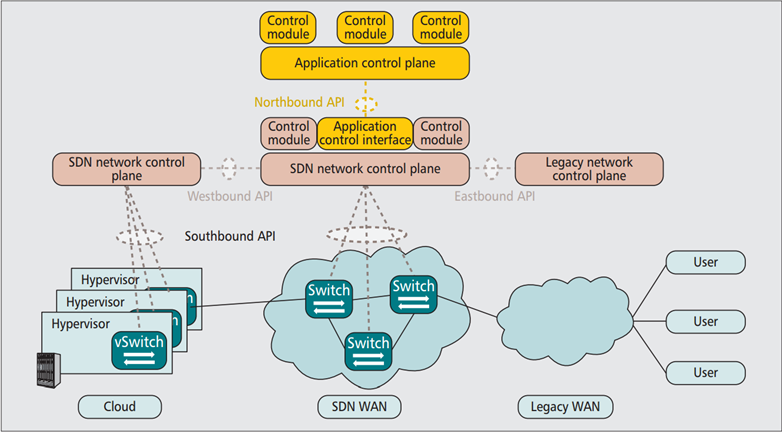
\includegraphics[width=13cm]{figure/ONF.png}
	\caption{The high-level SDN architecture.}
	\label{fig:{ONF}}
\end{figure}
\begin{itemize}
\item[] \textbf{Data Plane} : The data plane, or infrastructure plane, is the lowest layer in SDN architecture. This plane is composed by physical switches and virtual switches and others forwarding devices. Virtual switches are software-based switches, which can run on common operating systems. Open vSwitch \cite{OVS}, Indigo \cite{Indigo} and Pantou \cite{Pantou} are three implementations of virtual switches. Physical switches are hardware-based switches. They can be implemented on open network hardware (e.g., NetFPGA \cite{Lockwood2007}) or implemented on networking hardware vendors’ merchant switches. Many networking hardware vendors such as HP, NEC, Huawei, Juniper and Cisco, have supported SDN protocols. Virtual switches support complete features of SDN protocols, while physical switches lack the flexibility and feature completeness. However, physical switches have a higher flow forwarding rate than virtual switches.  SwitchBlade \cite{Anwer2010} and ServerSwitch \cite{Lu2011} are two NetFPGA-based physical switches.
These switches in data plane are responsible for forwarding, dropping and modifying packets based on instructions received from the Control Plane (CP) through Southbound Interfaces (SBIs).
\item[] \textbf{Control Plane}: The control plane is the “brain” of SDN systems, which can define network resources, dynamically choose forwarding rules and make network administration flexible and agile. The controller is responsable of many relevant tasks like:
\begin{itemize}
\item[•] the communication between forwarding devices and applications;
\item[•] it exposes and abstracts network state information of the data plane to the application plane;
\item[•] it translates the requirements from applications into custom policies and distributes them to forwarding devices;
\item[•] provides essential functionalities that most of network applications need, such as shortest path routing, network topology storage, device configuration and state information notifications etc.
\end{itemize}
There are many controller architectures, such as Ryu \cite{RYU}, OpenDayLight, \cite{Medved2014} NOX \cite{NOX}, POX \cite{POX}, Floodlight \cite{Floodlight} and Beacon \cite{Erickson2013}. Three communication interfaces allow the controllers to interact: southbound, northbound (NBI) and eastbound/westbound interfaces.
The	SBIs are defined between the control plane and the data plane. They allow forwarding devices to exchange network state information and control policies with the CP and provide functions such as statistics reports, forwarding operations, programmatic control of all device-capability advertisements and event notifications. OpenFlow \cite{McKeown2008} promoted by ONF is the first and the most popular open standard SBI. There exist other less popular proposals such as OVSDB \cite{OVS_Pfaff}, Protocol-Oblivious Forwarding (POF) \cite{Song2013} and OpenState \cite{Bianchi2014}. With NBIs, automation, innovation and management of SDN networks has been facilitate thanks to the fact that applications can exploit the abstract network views provided by the CP. The ONF is trying to define the standard NBIs and a common information model.
The eastbound/westbound interfaces are used in the multi-controller SDN networks. Due to the vast amount of data flows in such networks and the limited processing capacity of one controller the large-scale networks are always partitioned into several domains and each domain has its own controller.
The eastbound/westbound interfaces are responsible for the communication among multiple controllers. This communication  is necessary to exchange information in order to provide a global network view to the upper-layer applications. Onix \cite{Koponen} and HyperFlow \cite{Tootoonchian} are two distributed control architectures. Because their eastbound/westbound interfaces are private, they cannot communicate with each other. To enable the communication between different types of SDN controllers, SDNi \cite{yin2012}, East-West Bridge \cite{Lin2013} and Communication Interface for Distributed Control plane (CIDC) \cite{Benamrane2017} have been proposed as eastbound/westbound interfaces to exchange network information. However, the eastbound/westbound interfaces have not yet been standardized.
\item []\textbf{Application Plane}: The highest layer in the SDN architecture is the application plane. These applications can provide new services and perform business management, optimization and can obtain the required network state information through controllers’ NBIs. Based on the received information and other requirements, the applications can apply some control logic to change network behaviors.
The SDN-based applications have attracted a lot of attention from academia. Mendiola et al. \cite{Mendiola2017} have discussed the impact of SDN on Traffic Engineering (TE) and surveyed the SDN-based TE solutions. Security in SDN has been surveyed in \cite{Ahmad2015, ScottHayward2016, Rawat2017, Ali2015, Yan2016, Dargahi2017}. Especially, Yan et al. \cite{Yan2016} have researched on Distributed Denial of Service (DDoS) attacks in SDN-based cloud computing systems, and discussed future research challenges. Fault management in SDN has been surveyed in \cite{Fonseca2017}, which gives an identification and classification of the main fault management issues, and does valuable surveys and discussions about efforts that address those issues. Guck et al. \cite{Guck2018} have studied the centralized QoS routing mechanisms in SDN, and introduced a novel Four-Dimensional (4D) evaluation framework.
SDN has been deployed in many networks, such as transport networks \cite{Alvizu2017}, optical networks \cite{Thyagaturu2016}, wireless networks \cite{Haque2016, Chen2015}, Internet of Things (IoT) \cite{Bera2017}, edge computing \cite{Baktir2017}, Wide Area Networks (WAN) \cite{Michel2017}, cloud computing \cite{Jain2013}, Network Function Virtualization (NFV) \cite{Li2015, Liang2015}.
\end{itemize}
For more informations on SDN, please refer to \cite{Nunes2014, Jarraya2014, Xia2015, Hu2014, Xie2015, Trois2016, Huang2017, Blenk2016}.


\subsection{Workflow}
To understand the SDN architecture, it is important to recall its basic operation. Figure \ref{fig:{WorkFlow}} shows the working procedure of the OpenFlow-based SDN network \cite{OFP13}. Each OpenFlow switch has a flow table and uses the OpenFlow protocol to communicate with the SDN controller. The messages transmitted between the OpenFlow-based switches and the software-based controller are standardized by the OpenFlow protocol \cite{Erickson2013}. The OpenFlow controller can manage the traffic forwarding by modifying flow entries in switches flow tables.
\begin{figure}[tb!]
	\centering
	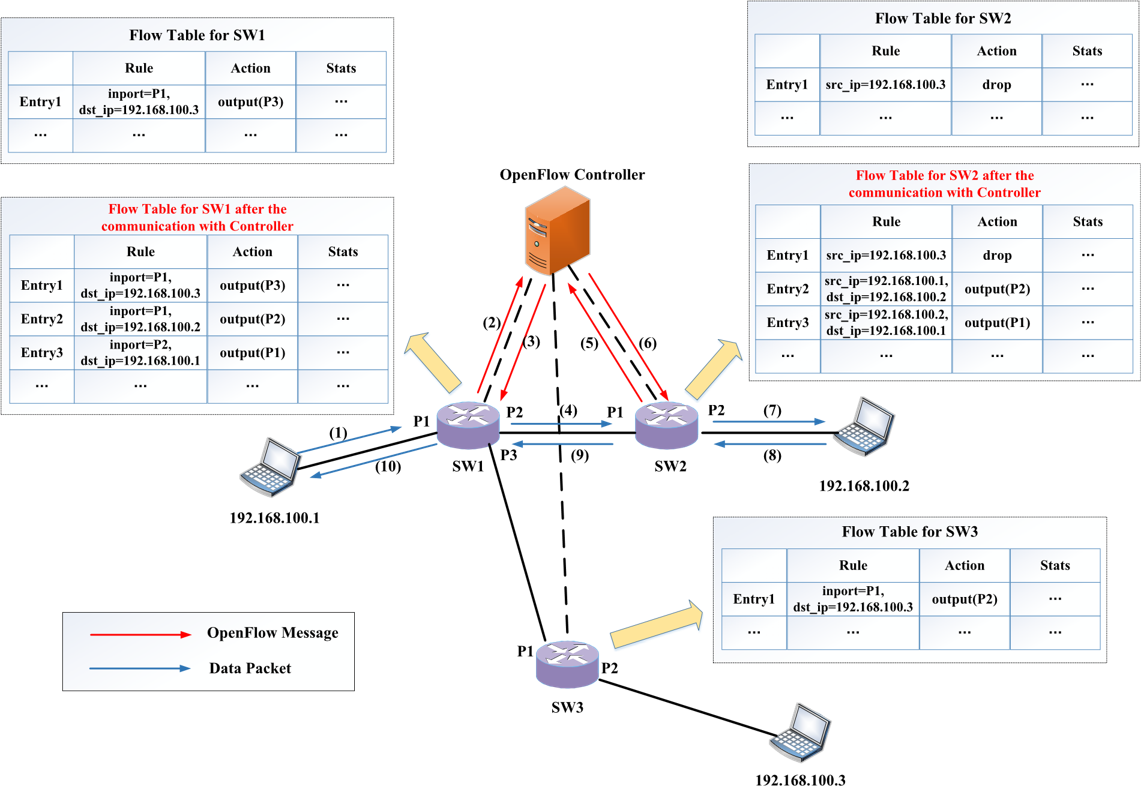
\includegraphics[width=13cm]{figure/WorkFlow.png}
	\caption{Example of OpenFlow-based SDN network.}
	\label{fig:{WorkFlow}}
\end{figure}
The flow table in the OpenFlow switch is comprised of flow entries to determine the processing actions of different packets on the data plane. When an OpenFlow switch receives a packet on the data plane, the packet header fields will be extracted and matched against flow entries. If a matching entry is found, the switch will process the packet locally according to the actions in matched flow entry. Otherwise, the switch will forward an OpenFlow PacketIn message to the controller (arrows 2 and 5). The packet header (or the whole packet, optionally) is included in the OpenFlow PacketIn message. Then, the controller will send OpenFlow FlowMod messages to manage the switch’s flow table by adding flow entries (arrows 3 and 6), which can be used to process subsequent packets of the flow.  For example, by adding two flow entries (i.e., Entry2 and Entry3) at SW1 and SW2, the communications between $192.168.100.1$ and $192.168.100.2$ are allowed.
However, packets from $192.168.100.3$ to $192.168.100.2$ are denied at SW2 due to security policies.
%====================================================================================================
%====================================================================================================
\section{Overview Of Machine Learning Algorithms} \label{sec:ML_BGK}
Machine learning is evolved from a collection of powerful techniques in AI areas. These methods start from training data to learn useful structural patterns and models. A machine learning approach consists of two main phases: the training phase and the decision making phase. In the training phase, after a data mining period that creates a training dataset, machine learning methods are applied to learn a system model. In the decision making phase, the trained model is used to estimate the output corresponding to each new input.
Machine learning algorithms can be distinguished into four main categories: supervised, unsupervised, semi-supervised and reinforcement learning.
\begin{figure}[tb!]
	\centering
	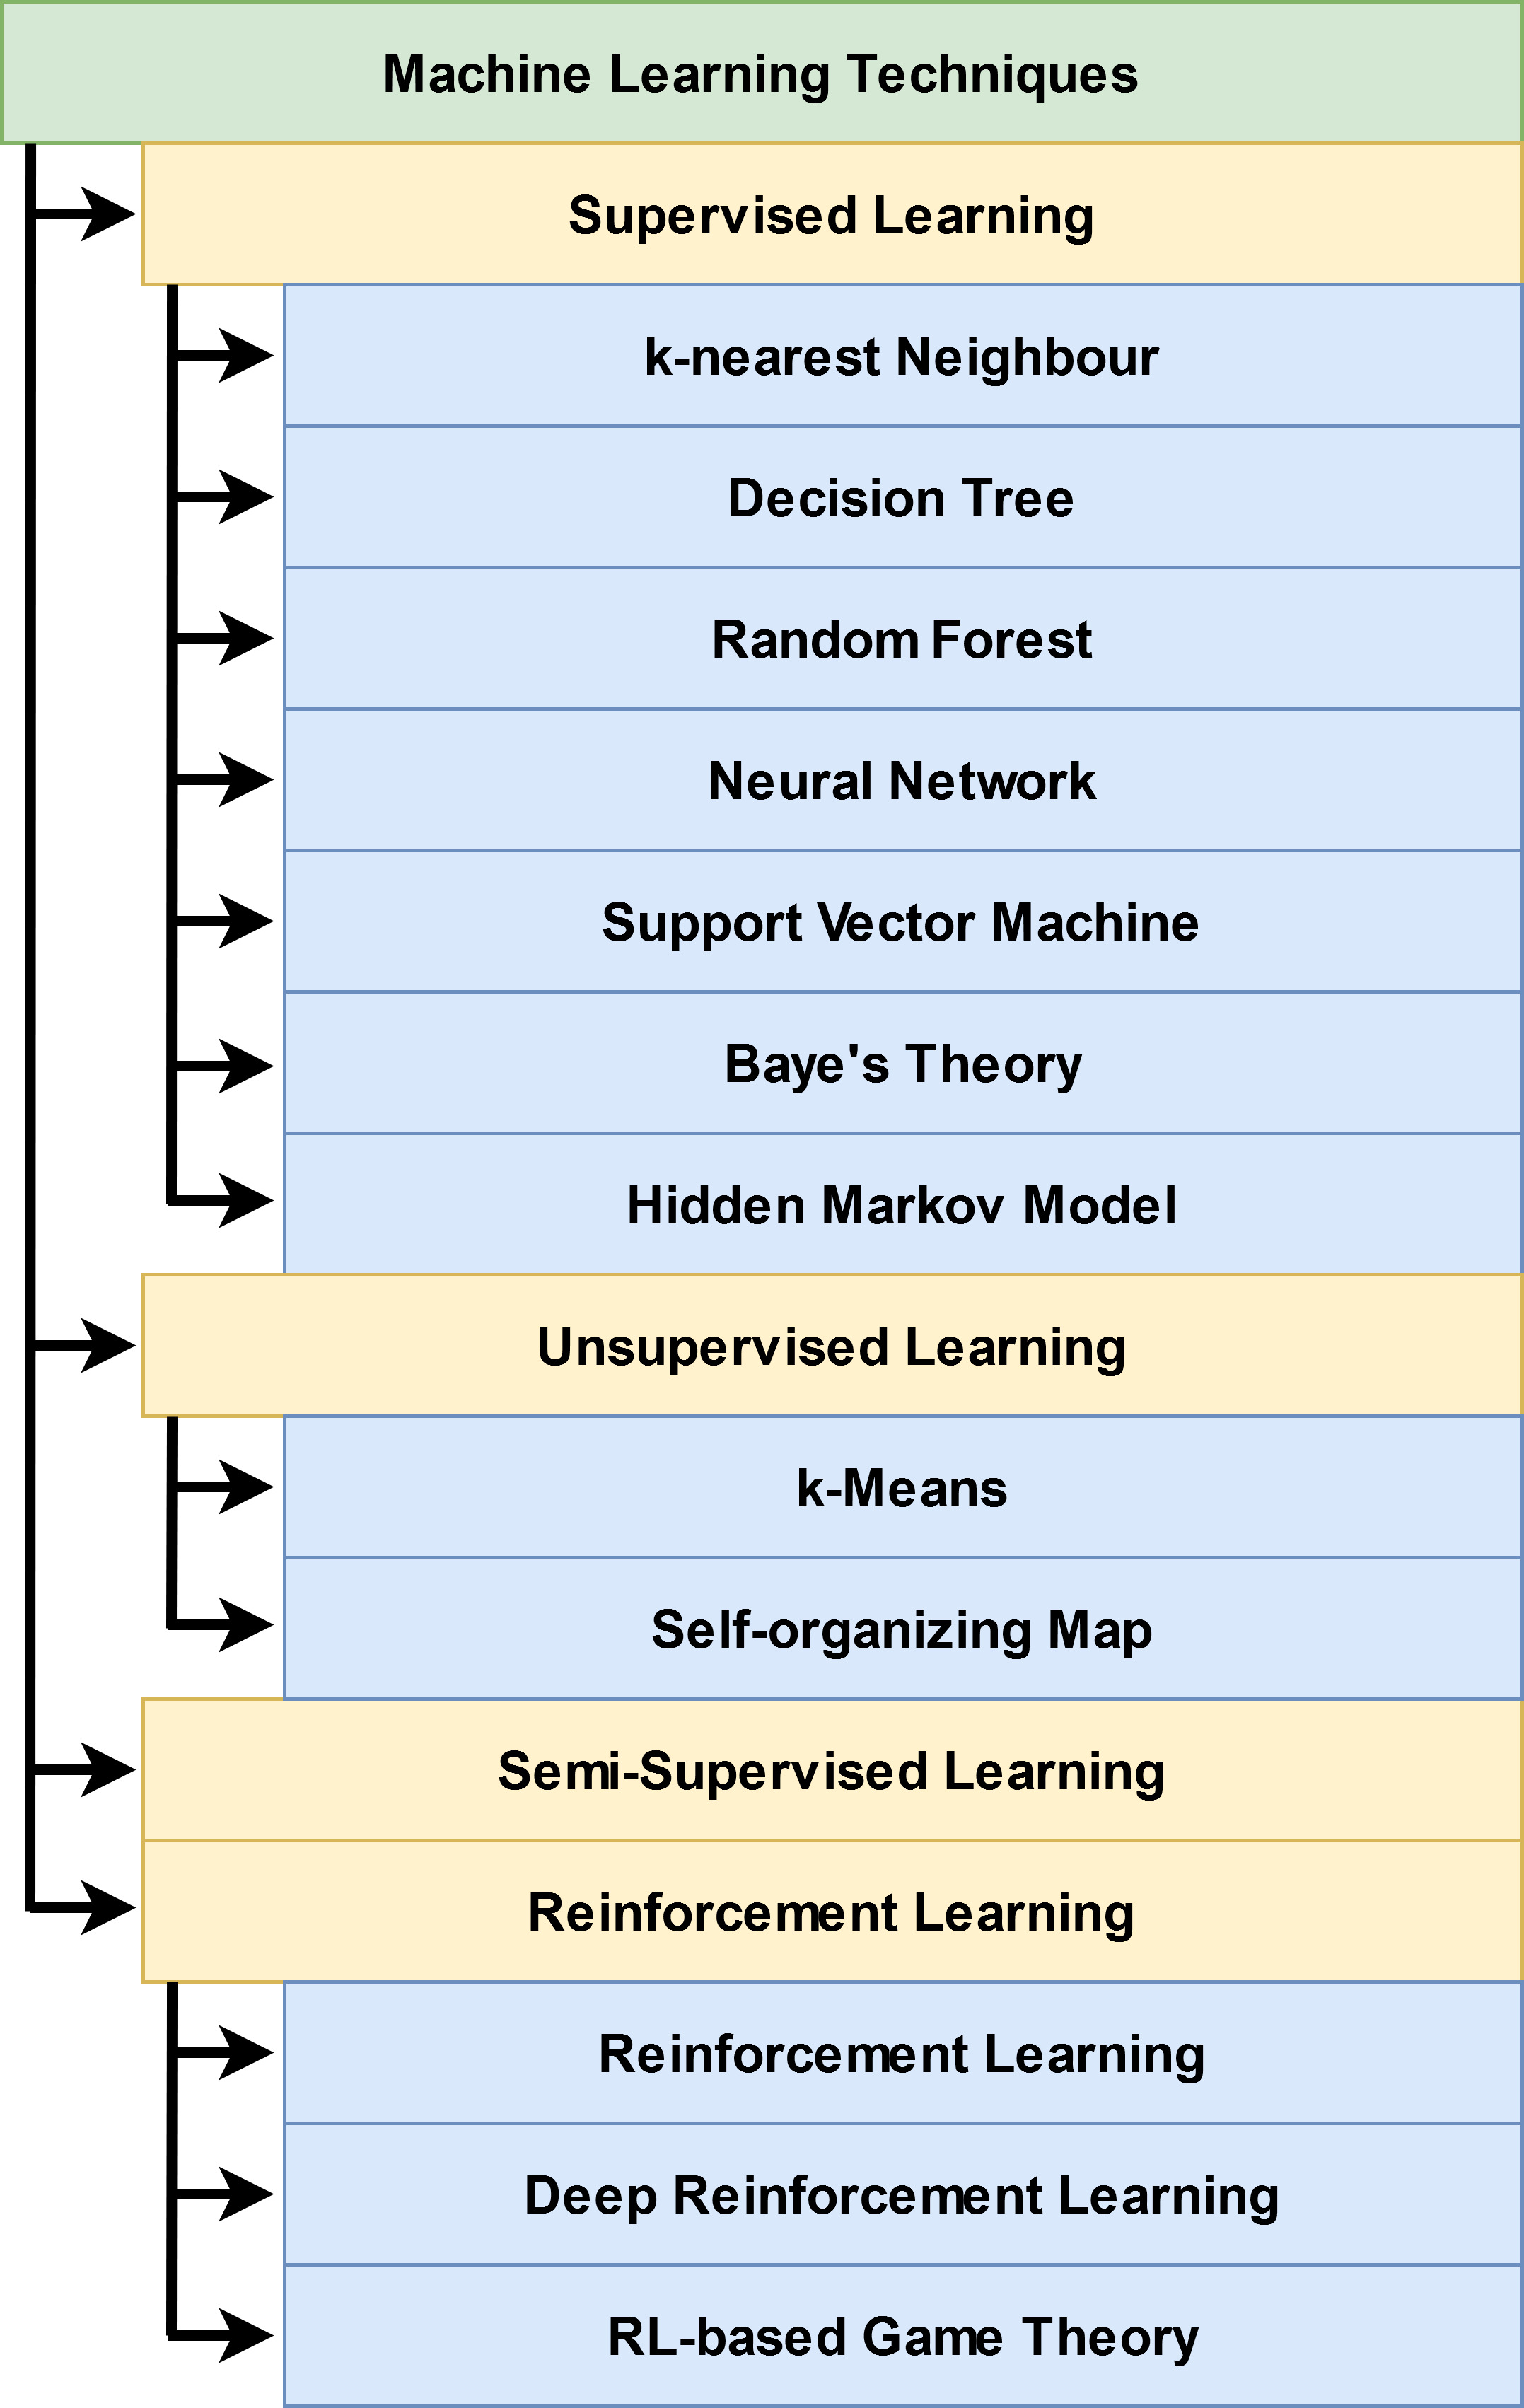
\includegraphics[scale=0.13]{figure/ML_algo.jpg}
	\caption{Common machine learning algorithms.}
	\label{fig:{ML_algo}}
\end{figure}
Each algorithm in Figure \ref{fig:{ML_algo}} is briefly explained with some examples. For a more insightful discussion on machine learning theory, please refer to \cite{Mohammed2016, Marsland2015, Alpaydin2020}.

\subsection{Supervised Learning}
Supervised learning is a kind of labelling learning technique. Supervised learning algorithms are given a labeled training dataset (i.e., inputs and known outputs) to build the system model representing the learned relation between the input and output. After training, when a new input is fed into the system, the trained model can be used to get the expected output \cite{Kotsiantis2007, Hastie2009}. In the following, an exhaustive representation of supervised learning algorithms is provided:
\begin{itemize}
\item[]\textit{1) k-Nearest Neighbor} (k-NN): In k-NN the classification of a data sample is determined based on the k nearest neighbors of that unclassified sample. The process of the k-NN algorithm is very simple: if the most of the k nearest neighbors belong to a certain class, the unclassified sample will be classified into that class. The higher the value of k is, the less effect the noise will have on the classification. Since the distance is the main metric of the k-NN algorithm, several functions can be applied to define the distance between the unlabeled sample and its neighbors, such as Chebyshev, City-block, Euclidean and Euclidean squared \cite{Cover1967}.
\item[]\textit{2) Regresstion Tree}: The RT performs classification through a learning tree. In the tree, each node represents a data feature, all branches represent the conjunctions of features that lead to classifications, and each leaf node is a class label. The unlabeled sample can be classified by comparing its feature values with the nodes of the RT \cite{Han2011}. The RT has many advantages, such as intuitive knowledge expression, simple implementation and high classification accuracy. ID3 \cite{Quinlan1986}, C4.5 \cite{Karatsiolis2012} and CART \cite{Burrows1995} are three widely-used decision tree algorithms. The biggest difference among them is the splitting criteria which are used to build decision trees. 
\item[]\textit{3) Random Forest}: A RF \cite{Breiman1999} consists of many RT. To mitigate over-fitting of RT methods and improve accuracy, the random forest method construct each RT by randomly choosing a subset of the features space . The steps to classify a new data sample by using random forest methods are:
\begin{itemize}
\item[]a) Put the data sample in each tree in the forest;
\item[](b) Each tree gives a classification result (vote);
\item[](c) The data sample will be classified into the class which has more votes.
\end{itemize}
\item[]\textit{4) Neural Network} (NN): A neural network is a computing system composed by a large number of simple processing units, which operate in parallel to learn experiential knowledge from historical data \cite{Haykin}. Each neuron performs highly complex, nonlinear and parallel computations. In a NN, its nodes are the equivalent components of the neurons in the human brain. These nodes use activation functions to perform nonlinear computations. The most frequently used activation functions are the sigmoid and the hyperbolic tangent functions. Simulating the way neurons are connected in the human brain, the nodes in a NN are connected to each other by variable link weights.
A NN has many layers. The first layer is the input layer, the last layer is the output layer and layers between them are the hidden layers. The output of each layer is the input of the next layer and the output of the last layer is the result. By changing the number of hidden layers and the number of nodes in each layer, complex models can be trained to improve the performance of NNs. NNs are widely used in many applications, such as pattern recognition. In figure \ref{fig:{NN_base}} the most basic NN with three layers has been shown. An input has $m$ features (i.e., $X_{1},X_{2},...,X_{m}$) and the input can be assigned to n possible classes (i.e., $Y_{1},Y_{2},...,Y_{n}$). Also, $W_{ij}^{1}$ denotes the variable link weight between the $ith$ neuron of layer $l$ and the $jth$ neuron of layer $l + 1$, and $ak^{l}$ denotes the activation function of the $kth$ neuron in layer $l$.
\begin{figure}[tb!]
	\centering
	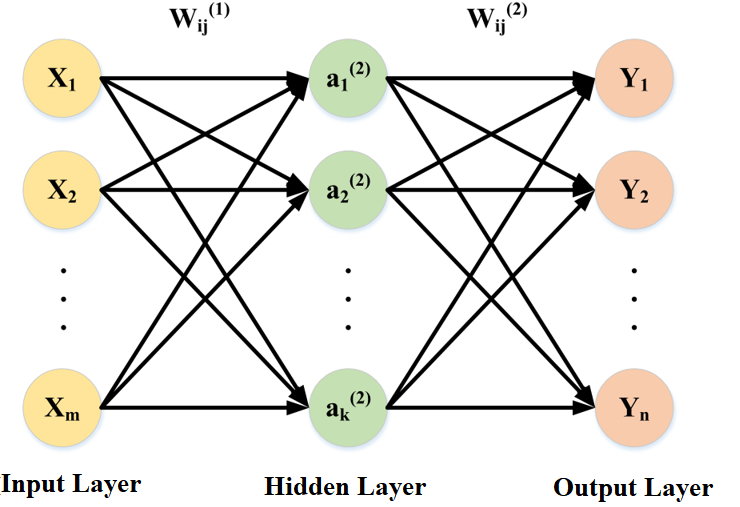
\includegraphics[width=13cm]{figure/NN_base.png}
	\caption{A basic neural network with three layers: an input layer, a hidden layer and an output layer.}
	\label{fig:{NN_base}}
\end{figure}
There are many types of neural networks, which can be divided in supervised or unsupervised main group \cite{Lee2005}. In the following, we will give a brief description of supervised neural networks.
\begin{itemize}
\item[]\textit{a)	Random NN}: The random NN can be represented as an interconnected network of neurons that exchange spiking signals. The main difference between random NN and other neural networks is that neurons in random NN exchange spiking signals probabilistically. In random NN, the internal excitatory state of each neuron is represented by an integer called “potential”. The potential value of each neuron rises when it receives an excitatory spiking signal and drops when it receives an inhibitory spiking signal. Neurons whose potential values are strictly positive are allowed to send out excitatory or inhibitory spiking signals to other neurons according to specific neurondependent spiking rates. When a neuron sends out a spiking signal, its potential value drops one. The random NN has been used in classification and pattern recognition \cite{Timotheou2010}.
\item[]\textit{b)	Deep NN}: Neural networks with a single hidden layer are generally referred to as shallow NNs. In contrast, neural networks with multiple hidden layers between the input layer and the output layer are called deep NNs \cite{LeCun2015, Schmidhuber2015}. To process high-dimensional data and to learn increasingly complex models, deep NNs with more hidden layers and neurons are needed. However, deep NNs increase the training difficulties and require more computing resources. In recent years, the development of hardware data processing capabilities and the evolved activation functions make it possible to train deep NNs \cite{Pandey2014}. In deep NNs, each layer’s neurons train a feature representation based on the previous layer’s output, which is known as feature hierarchy. The feature hierarchy makes deep NNs capable of handling large high-dimensional datasets. Due to the multiple-level feature representation learning, compared to other machine learning techniques, deep NNs generally provide much better performance \cite{Pandey2014}.
\item[]\textit{c)	Convolutional NN}: Convolutional NN and recurrent NN are two major types of deep NNs. Convolutional NN \cite{Krizhevsky2012, Li2018} is a feed-forward neural network. Local sparse connections among successive layers, weight sharing and pooling are three basic ideas of convolutional NN. Weight sharing means that weight parameters of all neurons in the same convolution kernel are same. Local sparse connections and weight sharing can reduce the number of training parameters. Pooling can be used to reduce the feature size while maintaining the invariance of features. The three basic ideas reduce the training difficulties of convolutional NNs greatly.
\item[]\textit{d)	Recurrent NN}: In feed-forward neural networks, the information is transmitted directionally from the input layer to the output layer. However, recurrent NN is a stateful network, which can use internal state (memory) to handle sequential data. Unlike a traditional deep NN, which uses different parameters at each layer, the recurrent NN shares the same parameters across all time steps. This means that at each time step, the recurrent NN performs the same task, just with different inputs. In this way, the total number of parameters needed to be trained is reduced greatly. Long Short-Term Memory (LSTM) \cite{Li2015a} is the most commonly-used type of recurrent NNs, which has a good ability to capture long-term dependencies. LSTM uses three gates (i.e., an input gate, an output gate and a forget gate) to compute the hidden state.
\end{itemize}
\item[]\textit{5) Support Vector Machine} (SVM): SVM is invented by Vapnik and others \cite{Vapnik1999}, which has been widely used in classification and pattern recognition. The basic idea of SVM is to map the input vectors into a high-dimensional feature space. This mapping is achieved by applying different kernel functions, such as linear, polynomial and Radial Based Function (RBF). Kernel function selection is an important task in SVM, which has effect on the classification accuracy. The selection of kernel function depends on the training dataset. The linear kernel function works well if the dataset is linearly separable. If the dataset is not linearly separable, polynomial and RBF are two commonly-used kernel functions. In general, the RBF-based SVM classifier has a relatively better performance than the other two kernel functions.
The objective of SVM is to find a separating hyperplane in the feature space to maximize the margin between different classes. The margin is the distance between the hyperplane and the closest data points of each class. The corresponding closest data points are defined as support vectors.
\item[]\textit{6) Bayes’ Theory}: Bayes’ theory uses the conditional probability to calculate the probability of an event occurring given the prior knowledge of conditions that might be related to the event. The Bayes’ theory is defined mathematically as the following equation:
\begin{equation*}
P(H\vert E)=\dfrac{P(E\vert H)P(H)}{P(E)}
\end{equation*}
where $E$ is a new evidence, $H$ is a hypothesis, $P(H\vert E)$ is the posterior probability that the hypothesis $H$ holds given the new evidence $E$, $P(E\vert H)$ is the posterior probability that of evidence $E$ conditioned on the hypothesis $H$, $P(H)$ is the prior probability of hypothesis $H$, independent of evidence $E$, and $P(E)$ is the probability of evidence $E$.
In a classification problem, the Bayes’ theory learns a probability model by using the training dataset. The evidence $E$ is a data sample, and the hypothesis $H$ is the class to assign for the data sample. The posterior probability $P(H\vert E)$ represents the probability of a data sample belonging to a class. In order to calculate the posterior probability $P(H\vert E)$, $P(H)$, $P(E)$ and $P(E\vert H)$ need to be calculated first based on the training dataset using the probability and statistics theories, which is the learning process of the probability model. When classifying a new input data sample, the probability model can be used to calculate multiple posterior probabilities for different classes. The data sample will be classified into the class with the highest posterior probability $P(H\vert E)$. The advantage of Bayes’ theory is that it requires a relatively small number of training samples dataset to learn the probability model \cite{Box2011}. However, there is an important independence assumption when using the Bayes’ theory. To facilitate the calculation of $P(E\vert H)$, the features of data samples in the training dataset are assumed to be independent of each other \cite{Bakker2017}.
\item[]\textit{7) Hidden Markov Models} (HMM): HMM is one kind of Markov models. Markov models are widely used in randomly dynamic environments which obey the 
memoryless property. The memoryless property of Markov models means that the conditional probability distribution of future states only relates to the value of the current state and is independent of all previous states \cite{Rabiner1989, Holgado2020}. There are other Markov models, such as Markov Chains (MC). The main difference between HMM and other models is that HMM is often applied in environments where system states are partially visible or not visible at all.
\end{itemize}
\subsection{Unsupervised Learning}
In contrast to supervised learning, an unsupervised learning algorithm is given a set of inputs without labels, thus there is no output. An unsupervised learning algorithm aims to find patterns, structures, or knowledge in unlabeled data by clustering sample data into different groups according to the similarity between them. The unsupervised learning techniques are widely used in clustering and data aggregation. In the following, we will give a representation of widely-used unsupervised learning algorithms.
\begin{itemize}
\item[]\textit{1)	k-Means}: The k-means algorithm is used to recognize a set of unlabeled data into different clusters. To implement the kmeans algorithm, only two parameters are needed: the initial dataset and the desired number of clusters. If the desired number of clusters is k, the steps to resolve node clustering problem by using k-means algorithms are:
\begin{itemize}
\item[]\textit{a)} initialize k cluster centroids by randomly choosing k nodes;
\item[]\textit{b)} use a distance function to label each node with the closest centroid;
\item[]\textit{c)} assign new centroids according to the current node memberships;
\item[]\textit{d)} stop the algorithm if the convergence condition is valid, otherwise go back to step \textit{b)}.
\end{itemize}
\item[]\textit{2)	Self-Organizing Map} (SOM): SOM, also known as SelfOrganizing Feature Map (SOFM) \cite{Kohonen2012}, is one of the most popular unsupervised neural network models. SOM is often applied to perform dimensionality reduction and data clustering. In general, SOM has two layers, an input layer and a map layer. When SOM is used to perform data clustering, the number of neurons in the map layer is equal to the desired number of clusters. Each neuron has a weight vector. The steps to resolve data clustering problem by using SOM algorithm are:
\begin{itemize}
\item[]a) initialize the weight vector of each neuron in the map layer;
\item[](b) choose a data sample from the training dataset;
\item[](c) use a distance function to calculate the similarity between the input data sample and all weight vectors. The neuron whose weight vector has the highest similarity is called the Best Matching Unit (BMU). The SOM algorithm is based on competitive learning;
\item[](d) The neighborhood of the BMU is calculated;
\item[](e) The weight vectors of the neurons in the BMU’s neighborhood are adjusted towards the input data sample;
\item[](f) Stop the algorithm if the convergence condition is valid, otherwise go back to step (b).
\end{itemize}
\end{itemize}
\subsection{Semi-Supervised Learning}
Semi-supervised learning is a type of learning which uses both labeled and unlabeled data. Semi-supervised learning is useful due the fact that in many real-world applications, the acquisition of labeled data is expensive and difficults while acquiring a large amount of unlabeled data is relatively easy and cheap. Moreover effective use of unlabeled data during the training process actually tends to improve the performance of the trained model. In order to make the best use of unlabeled data, assumptions have to be hold in semisupervised learning, such as smoothness assumption, cluster assumption, low-density separation assumption, and manifold assumption. Pseudo Labeling \cite{Wu2018} is a simple and efficient semi-supervised learning technique. The main idea of Pseudo Labeling is simple. Firstly, use the labeled data to train a model. Then, use the trained model to predict pseudo labels of the unlabeled data. Finally, combine the labeled data and the newly pseudo-labeled data to train the model again. There are other semi-supervised learning methods, such as Expectation Maximization (EM), co-training, transductive SVM and graph-based methods. Different methods rely on different assumptions. For example, EM builds on cluster assumption, transductive SVM builds on low-density separation assumption, while graph-based methods build on the manifold assumption.
\subsection{Reinforcement Learning}
Supervised learning algorithms are generally applied to conduct classification and regression tasks, while unsupervised and reinforcement learning algorithms are applied to conduct clustering and decision-making tasks respectively.
\begin{itemize}
\item[]\textit{1)	Reinforcement Learning} (RL): RL \cite{Sutton2018, Kaelbling1996} involves an agent, a state space S and an action space A. The agent is a learning entity which interacts with its environment to learn the best action to maximize its long-term reward. The long-term reward is a cumulative discounted reward and relates to both the immediate reward and future rewards. When applying RL to SDN, the controller generally works as an agent and the network is the environment. The controller monitors the network status and learns to make decisions to control data forwarding. Specifically, at each time step $t$, the agent monitors a state $s_{t}$ and chooses an action $a_{t}$ from the action space $A$, receives an immediate reward $r_{t}$ which indicates how good or bad the action is, and transitions to the next state $st+1$. The objective of the agent is to learn the optimal behavior policy $\pi$ which is a direct map from the state space S to the action space $A (\pi : S \longrightarrow A)$ to maximize the expected long-term reward. From the behavior policy $\pi$, the agent can determine the best corresponding action given a particular state. In RL, value function is used to calculate the long-term reward of an action given a state. The most well-known value function is Q-function, which is used by Q-learning to learn a table storing all state-action pairs and their long-term rewards.
\item[]\textit{2)	Deep Reinforcement Learning} (DRL): The main advantage of RL is that it works well without prior knowledge of an exact mathematical model of the environment. However, the traditional RL approach has some shortcomings, such as low convergence rate to the optimal behavior policy $\pi$ and its inability to solve problems with high-dimensional state space and action space. These shortcomings can be addressed by DRL. The key idea of DRL is to approximate the value function by leveraging the powerful function approximation property of deep NNs. After training the deep NNs, given a state-action pair as input, DRL is able to estimate the long-term reward. The estimation result can guide the agent to choose the best action.
\item[]\textit{3)	RL-Based Game Theory}: Game theory is a mathematical tool that focuses on strategic interactions among rational decision-makers. A game generally involves a set of players, a set of strategies and a set of utility functions. Players are decision-makers. Utility functions are used by players to select optimal strategies. In cooperative games, players cooperate and form multiple coalitions. Players choose strategies that maximize the utility of their coalitions. In non-cooperative games, players compete against each other and choose strategies individually to maximize their own utility. In the network field, it is often assumed that nodes are selfish.
In non-cooperative games, players do not communicate with each other, and at the beginning of each play round, players do not have any information about the strategies selected by the other players. At the end of each play round, all players broadcast their selected strategies, which are the only external information. However, each player’s utility can be affected by the other players’ strategies. In this case, adaptive learning methods should be used to predict the strategies of the other players, based on which each player chooses its optimal strategy. RL is a widely-used adaptive learning method, which can help players select their optimal strategies by learning from historical information such as network status, the other players’ strategies and the corresponding utility. Thus, RL-based game theory is an effective decision-making technique.
\end{itemize}

%====================================================================================================

%\newpage
\section{Switched affine modeling via RT and RF}\label{secSwitchedModeling}
%====================================================================================================

\textbf{\emph{Problem formulation.}} In this section it is illustrated the methodology to apply the results proposed in \cite{SmarraADHS2018,smarraNAHS2020} to identify, starting from a set of collected historical data $ \mathcal{D}=\{y(k),u(k),d(k)\}_{k = 0}^{\ell} $ as illustrated in the previous section, a switching ARX model of input-output behavior of the traffic flow in a switch of a SDN network as follows:
%The aim of such predictive model is to enable the direct and computationally efficient implementation of Model Predictive Control for bandwidth and packet losses optimisation.
\small
\begin{equation}\label{eqIdentifiedModelNSARX}
x(k+j+1) =	A'_{\sigma_j(x(k),d(k))} x(k) + \sum_{\alpha = 0}^{j}B'_{\sigma_{j}(x(k),d(k)),\alpha} u(k+\alpha) + f'_{\sigma_j(x(k),d(k))},
\end{equation}
\normalsize
\noindent $j = 0,\ldots, N-1$, where $x(k) \doteq [y^\top(k)\ \cdots\ y^\top(k-\delta_y)\ u^\top(k-1)\ \cdots\ u^\top(k-\delta_u)]^\top\in\Real^{n_x}$ is an extended state to characterize a switching ARX model, with $x_\iota(k) \doteq [y_\iota(k)\ \cdots\ y_\iota(k-\delta_y)\ u^\top(k-1)\ \cdots\ u^\top(k-\delta_u)]^\top\in\Real^{\delta_y+1+3\delta_u}$, $\iota = 1,2,3$, $N$ is the chosen future predictive horizon, and  $\sigma_j : \mathbb{R}^{n_x+10} \to \mathcal M \subset \mathbb{N}$ is a switching signal that associates an operating mode in a finite set $\mathcal M$ to each pair $(x(k),d(k))$ and each prediction step $j$ of the horizon.
It is possible to directly use model \eqref{eqIdentifiedModelNSARX} to setup the following problem, which can be solved using standard Quadratic Programming (QP) solvers:\\
\begin{problem}\label{pbMPCSwitching}
	\small
	\vspace{-0.3cm}
	\begin{equation*}
		\begin{aligned}
			& \underset{u_0,\ldots,u_{N-1}}{\text{minimize}} & &  \sum_{j=0}^{N-1} \left(\left(x_{j+1}-x_{\mathrm{ref}}\right)^\top Q \left(x_{j+1}-x_{\mathrm{ref}}\right) + u^\top_{j} R u_{j}\right)\\
			& \text{subject to }            & &  x_{j+1} = A'_{\sigma_j(x_{0},d_{0})} x_0 + \sum_{\alpha = 0}^{j}B'_{\sigma_{j}(x_{0},d_{0}),\alpha} u_\alpha + f'_{\sigma_j(x_{0},d_{0})}\\       
			&                               & &  u_{j}   \in \mathcal{U}\\
			&                               & &  x_{0} = x(k), d_{0} = d(k)\\ 
			&                               & &  j = 0,\ldots,N-1.			\\
		\end{aligned}
		\vspace{0.1cm}
	\end{equation*}
	\normalsize
\end{problem}
\noindent As it is well known \cite{borrelli2017predictive}, Problem \ref{pbMPCSwitching} is solved at each time step $k$ using QP to compute the optimal sequence $u^*_0,\ldots,u^*_{N-1}$, but only the first input is applied to the system, i.e. $u(k) = u^*_0$. Note that, for any prediction step $j$, $x_{j+1}$ only depends on the measurements $x_0=x(k),d_0=d(k)$ at time $k$, since they are the only available measurements at time-step $k$. 
%\subsection{Switching ARX Identification using RF}\label{secSARX}

%====================================================================================================

\textbf{\emph{RT and RF background.}} Let us consider a dataset $\{y(k),x_1(k),\ldots,x_\eta(k)\}_{k=0}^\ell$, with $y,x_1,\ldots,x_\eta\in\mathbb{R}$. Let us suppose  to estimate, using Regression Trees, the prediction of the (response) variable $y(k)$ using the values of predictor variables $x_1(k),\ldots,x_\eta(k)$. The CART algorithm \cite{BreimanCART2017} creates a RT structure via optimal partition of the dataset. It solves a Least Square problem by optimally choosing recursively a variable to split and a corresponding splitting point. After several steps the algorithm converges to the optimal solution, and the dataset is partitioned in hyper-rectangular regions (the leaves of the tree) $R_1, R_2,\cdots, R_\nu$. In each partition $y(k)$ is estimated with a different constant $\hat y_i\, i=1,\ldots,\nu,$ given by the average of the samples of $y(k)$ falling in $R_i$, i.e.

\begin{equation}\label{eqAverageResponseRT}
\hat y_{i} = \frac{\sum\limits_{\{k|(x_1(k),\ldots, x_\eta(k)) \in R_i\}}y(k)}{|R_i|}
\end{equation}


\noindent Random Forests \cite{BreimanML2001} are instead an averaging method that exploits a combination of tree predictors such that each tree depends on the values of a random vector sampled independently and with the same distribution for all trees in the forest. The output prediction is given by averaging the predictions provided by all trees in the forest. It is possible to show that the error introduced by the forests quickly and almost surely converges to a limit as the number of trees in the forest becomes large. Such error also depends on the strength of the individual trees in the forest and the correlation between them. Thus, due to the Law of Large Numbers, Random Forests (differently from Regression Trees) do not suffer much variance and overfitting problems. For more details the reader is refered to \cite{BreimanCART2017,BreimanML2001}.

%====================================================================================================

\textbf{\emph{Switching ARX (SARX) model identification via RT.}} To derive a model as in \eqref{eqIdentifiedModelNSARX}, a new dataset $\X= \{x(k),u(k),d(k)\}_{k = 0}^{\ell}$ has to be defined starting from $\D$. In order to apply MPC it is needed, for each component of $y(k)$, a model that can predict system's dynamics over a horizon of length $N$. The idea is to create $3 N$ predictive trees $\{\mathcal{T}_{\iota,j}\},\ \iota=1,2,3,\ j=0,\ldots,N-1$, each one to predict the 3 outputs components of the system over the $N$ steps of the horizon. To create the tree structure, the RT algorithm (CART) partitions the dataset $\X$ into regions $\X_i$, such that $\biguplus \X_i = \X$, and assigns to each region a constant value given by the average of the output values of the samples that ended up in that leaf. In run-time, once the trees are created, and given a real-time measurement $(x(k), u(k), d(k))$ belonging to leaf $i$, the CART algorithm provides as a prediction the averaged value associated to the leaf as in \eqref{eqAverageResponseRT}. However, since the prediction provided by the RT is a constant value, it cannot be used to setup an MPC problem, thus the learning procedure needs to be modified to identify a modeling framework as in \eqref{eqIdentifiedModelN}. To this end, $\X$ is partitioned in two disjoint sets $\mathcal{X}_c = \{u(k)\}_{k=0}^{\ell}$ of data associated to the control variables, and $\mathcal{X}_{nc} = \{(x(k), d(k))\}_{k=0}^{\ell}$ of data associated to remaining variables, and then apply the CART algorithm only on $\mathcal{X}_{nc}$ (this is to avoid that the MPC problem turns out into a Mixed Integer Quadratic Program, see \cite{SmarraADHS2018,smarraNAHS2020} for details); thus, $3 N$ RTs $\{\mathcal{T}_{\iota,j}\}$ have been created, each constructed to predict the variable $y_\iota(k+j+1)$, and consequently $x_\iota(k+j+1)$. In particular, it is associated to each leaf $\iota,i_j$, corresponding to the partition  $\mathcal{X}_{nc,\iota,i_j}$, of each tree $\mathcal{T}_{\iota,j}$ the following affine model

\small

\begin{equation}\label{eqLTIleavesSinglState}
	x_\iota(k+j+1) = A'_{\iota,i_j}x(k) + \sum_{\alpha = 0}^{j}{B'_{\iota,i_j,\alpha}u(k+\alpha)} + f'_{\iota,i_j},
\end{equation}
\normalsize
\small
\begin{equation}\label{eqLeafModel}
\begin{aligned}
A'_{\iota,i_j} =& \left[\begin{array}{cccccccccc}
a_1       & a_2       & \cdots & a_{\delta_y } & a_{\delta_y + 1} & b_{\delta_y + 2} & \cdots & b_{\delta_y + 1+ 3(\delta_u-1)} & \cdots & b_{\delta_y + 1 + 3\delta_u} \\
1         & 0         & \cdots & 0             & 0                & 0                & \cdots & 0                               & \cdots & 0                            \\
\vdots    & \vdots    & \ddots & \vdots        & \vdots           & 0                & \cdots & 0                               & \cdots & 0                            \\
0         & 0         & \cdots & 1             & 0                & 0                & \cdots & 0                               & \cdots & 0                            \\
0         & 0         & \cdots & 0             & 0                & 0                & \cdots & 0                               & \cdots & 0                            \\
0         & 0         & \cdots & 0             & 0                & 0                & \cdots & 0                               & \cdots & 0                            \\
0         & 0         & \cdots & 0             & 0                & 0                & \cdots & 0                               & \cdots & 0                            \\
0         & 0         & \cdots & 0             & 0                & 1                & \cdots & 0                               & \cdots & 0                            \\
\vdots    & \vdots    & \ddots & \vdots        & \vdots           & \vdots           & \ddots & \vdots                          & \ddots & \vdots                       \\
0         & 0         & \cdots & 0             & 0                & 0                & \cdots & 1                               & \cdots & 0                            \\

\end{array}\right],\\
B'_{\iota,i_j,\alpha} = & \left[\begin{array}{ccc}
b_{1,\alpha} & b_{2,\alpha} & b_{3,\alpha}\\
0            & 0            & 0            \\
\vdots       & \vdots       & \vdots \\
0            & 0            & 0            \\   
0            & 0            & 0            \\  
0            & 0            & 0            \\  
0            & 0            & 0            \\  
0            & 0            & 0            \\  
\vdots       & \vdots       & \vdots            \\   
0            & 0            & 0            \\   
\end{array}\right],\ \alpha<j,\ 
B'_{\iota,i_j,j} =  \left[\begin{array}{ccc}
b_{1,\alpha} & b_{2,\alpha} & b_{3,\alpha}\\
0            & 0            & 0            \\
\vdots       & \vdots       & \vdots \\
0            & 0            & 0            \\   
1            & 0            & 0            \\  
0            & 1            & 0            \\  
0            & 0            & 1            \\  
0            & 0            & 0            \\  
\vdots       & \vdots       & \vdots            \\   
0            & 0            & 0            \\   
\end{array}\right],\ 
f'_{\iota,i_j} = \left[\begin{array}{ccccc}
f      \\	0 \\ \vdots \\ 0 \\ 0 \\ 0 \\ 0 \\ 0 \\ \vdots \\ 0      
\end{array}\right],
\end{aligned}
\end{equation}
\normalsize

\noindent where the coefficients of matrices $A'_{\iota,i_j}$, $B'_{\iota,i_j,\alpha}$ and $f'_{\iota,i_j}$ are obtained in each leaf $\iota,i_j$ by fitting the corresponding set of samples solving the following Least Squares with inequality constraints problem:

\begin{problem}\label{pbLeastSquareProblem}
	\small
	\begin{alignat}{2}
		& \nonumber \underset{\xi_{\iota,i_j}}{\text{minimize}} & &  \parallel \Lambda_{\iota,i_j} \xi_{\iota,i_j}  - \lambda_{\iota,i_j} \parallel_2^2   		 \\
		& \text{subject to }    \nonumber            & &  f_\mathrm{min} \leq f \leq f_\mathrm{max}    										  					 \\
		&                  					    	 & &  a_\mathrm{min} \leq a_{\jmath} \leq a_\mathrm{max}\label{eqInequalityConstraints} \\
		& 	                    \nonumber			 & &  b_\mathrm{min} \leq b_{\iota,\alpha} \leq b_\mathrm{max},
	\end{alignat}
	\normalsize
\end{problem}

\noindent where $\xi_{\iota,i_j}$, $\lambda_{\iota,i_j}$, and $\Lambda_{\iota,i_j}$ contain respectively the parameters of matrices in \eqref{eqLeafModel}, the predictions $x_\iota(k+j+1)$, and the current measurements of $x(k)$ and $u(k+\alpha)$. Linear inequalities \eqref{eqInequalityConstraints} are used to constrain elements in $\xi_{\iota,i_j}$ to take into account physical system constraints and improve prediction accuracy.
Model \eqref{eqLTIleavesSinglState} can be easily compacted in the following form taking into account all the states $\iota=1,2,3$:
\small
\begin{equation}\label{eqLTIleavesCompact}
x(k+j+1) = A'_{i_j}x(k) + \sum_{\alpha = 0}^{j}{B'_{i_j,\alpha}u(k+\alpha)} + f'_{i_j}.
\end{equation}
\normalsize
\noindent In particular, with the specific choice of $\delta_u = 0$ model \eqref{eqIdentifiedModelNSARX} can be rewritten in the following state-space formulation
\small
\begin{equation}\label{eqIdentifiedModelN}
x(k+j+1) =	A_{\sigma_j(x(k),\bold{u^-}(k),d(k))} x(k+j) + B_{\sigma_j(x(k),\bold{u^-}(k),d(k))} u(k+j) + f_{\sigma_j(x(k),\bold{u^-}(k),d(k))},
\end{equation}
\normalsize
where $\bold{u^-}(k) = [u^\top(k-1)\ \cdots\ u^\top(k-\delta)]^\top$ is the vector with the regressive terms of the input used to only grow the trees, and  $\sigma_j : \mathbb{R}^{3(\delta_y+1)+3\delta+10} \to \mathcal M \subset \mathbb{N}$.
%\noindent In particular, as anticipated in the problem formulation, with the specific choice of $\delta_u = 0$ matrices $A'_{\iota,i_j}$ in \eqref{eqLeafModel} modify as follows:
%
%\small
%\begin{equation}\label{eqLeafModelDelta_u=0}
%	\begin{aligned}
%		A'_{\iota,i_j} =& \left[\begin{array}{ccccc}
%			a_1       & a_2       & \cdots & a_{\delta_y } & a_{\delta_y + 1} \\
%			1         & 0         & \cdots & 0                         & 0     \\
%			\vdots    & \vdots    & \ddots & \vdots                    & \vdots     \\
%			0         & 0         & \cdots & 1                         & 0     
%		\end{array}\right]\\
%		B'_{\iota,i_j,\alpha} = & \left[\begin{array}{ccccc}
%			b_{1,\alpha} & 0 & \cdots & 0 & 0\\
%			b_{2,\alpha} & 0 & \cdots & 0 & 0           \\
%			b_{3,\alpha} & 0 & \cdots & 0 & 0           \\   
%		\end{array}\right]^\top\\
%				f'_{\iota,i_j} = &\left[\begin{array}{ccccc}
%		f      &	0 & \cdots & 0 & 0      
%		\end{array}\right]^\top.
%	\end{aligned}
%\end{equation}
%%\normalsize
Thanks to this new formulation the following proposition shows that model \eqref{eqLTIleavesCompact} is equivalent to model \eqref{eqIdentifiedModelN} for any initial condition, any switching signal and any control sequence.
\begin{proposition}\label{propSwitchingSystem}\cite{smarraNAHS2020}
	Let $A'_{i_j}$, $B'_{i_j,\alpha}$ and $f'_{i_j}$, $\alpha=0,\ldots,j$, $j=0,\ldots,N-1$, be given. If $A'_{i_j}$ is invertible for $j=0,\ldots,N-1$, then there exists a model in the form
	\vspace{-0.2cm}
	\small
	\begin{equation*}
	\bar x({k+j+1}) = A_{\sigma_j(\bar x(k),\bold{u^-}(k), d(k))} \bar x({k+j})+B_{\sigma_j(\bar x(k),\bold{u^-}(k), d(k))} u({k+j})+ f_{\sigma_j(\bar x(k),\bold{u^-}(k), d(k))}	
	\end{equation*}
	\normalsize
	such that for any initial condition $\bar x(k) = x(k) = x_k$, any switching sequence $i_0, \ldots, i_{N-1}$ and any control sequence $u(k),\ldots,u(k+N-1)$, then $\bar x(k+j+1) = x(k+j+1),\ \forall j=0,\ldots,N-1$.
\end{proposition}

As discussed in \cite{smarraNAHS2020}, from experimental findings it is possible to notice that the contribution in terms of model accuracy introduced by the choice of $\delta_u = 0$ is negligible, since previous control inputs are already considered in the tree structure choosing $\delta > 0$. Thus, in the rest of the paper it will be considered $\delta_u = 0$ and $\delta > 0$, i.e. only the regressive terms of the input in the tree structure learning will be used and not in the state definition.

\textbf{\emph{SARX model identification via RF.}} RF-based models can be constructed exploiting the RT-based formulation: in particular, let us consider $3 N$ RFs $\mathcal{F}_{\iota,j}$, $\iota = 1,2,3,\ j = 0,\ldots,N-1$. 
For each tree $\mathcal{T}^{\mathcal{F}_{\iota,j}}_\tau$ of the forest $\mathcal{F}_{\iota,j}$, it is possible to estimate the coefficients $a_*$, $b_*$ and $f$ in \eqref{eqLeafModel} for each leaf $\iota,j,i_\tau$, i.e. $\tilde\xi_{\iota,j,i_\tau}$, solving Problem \ref{pbLeastSquareProblem}.
With a small abuse of notation, let us indicate by $|\mathcal{F}_{\iota,j}|$ the number of trees in the forest ${\iota,j}$. 
Then $\forall \iota,j$, the parameters to build matrices in \eqref{eqLTIleaves} can be obtained by averaging parameters $a_*$, $b_*$ and $f$, $\forall \tau = 1,\ldots,|\mathcal{F}_{\iota,j}|$, i.e.
\small
\begin{equation}\label{eqAverageRF}
\tilde\xi_{\iota,j} = \frac{\sum\limits_{\tau=1}^{|\F_{\iota,j}|}\tilde\xi_{\iota,j,i_\tau}}{|\F_{\iota,j}|},
\end{equation}
\normalsize
over all the trees of forest $\F_{\iota,j}$. At this point, starting from \eqref{eqLTIleavesSinglState}, it can be easily construct the following model, as in \eqref{eqLTIleavesCompact} to be used in the MPC formulation by combining for $\iota=1,2,3$ the matrices in \eqref{eqLeafModel} coming either from the RTs or from the RFs:
\small
\begin{equation}\label{eqLTIleaves}
	x(k+j+1) = A'_{i_j}x(k) + \sum_{\alpha = 0}^{j}{B'_{i_j,\alpha}u(k+\alpha)} + f'_{i_j}.
\end{equation}
\normalsize

%====================================================================================================

\textbf{\emph{MPC problem formulation.}} It is used model \eqref{eqLTIleaves} to formalize Problem \ref{pbMPCSwitching} according to the SDN priority queueing problem:
\begin{problem}\label{pbMPC}

	\begin{equation*}
		\begin{aligned}
			& \underset{\bold u}
			{\text{minimize}}               & &  \sum_{j=0}^{N-1} \Big[(x_{j+1}-x_{\mathrm{ref},j})^\top Q (x_{j+1}-x_{\mathrm{ref},j}) + u^\top_{j} R u_{j}\Big]   \\
			& \text{subject to}             & &  x_{j+1}  =   A_{\sigma_j(k)} x_{j}+B_{\sigma_j(k)}  u_j+f_{\sigma_j(k)} \\
			&								& &  \Delta u_\iota^\mathrm{min} \leq u_{\iota,j} - u_{\iota,j-1} \leq \Delta u_\iota^\mathrm{max}             \\
			&								& &  u_\iota^\mathrm{min} \leq u_{\iota,j} \leq u_\iota^\mathrm{max}             \\
			&                               & &  u_{1,j} + u_{2,j} \leq 100			          		\\
			&                               & &  x_0 = x(k),\ \bold u^-_{0} = [u^\top(-1)\ \cdots\ u^\top(-\delta)]^\top,\ d_0 = d(k),\\
			&								& &  j = 0,\ldots,N-1,\ \iota = 1,2,3,                                 
		\end{aligned}
	\end{equation*}
	\normalsize
\end{problem}
\noindent where $\sigma_j(k) = \sigma_j(x(k),\bold{u^-}(k),d(k))$ (with a slight abuse of notation), $u_{\iota,j}$ is the $\iota^{th}$ component of the input $u$ at time $k+j$; $\Delta u_\iota^\mathrm{min}$ and $\Delta u_\iota^\mathrm{max}$ are used to limit large variations on the inputs in 2 consecutive steps, in order to avoid that the queues drastically set to the minimum value and thus potentially increase packet losses during the next period; $u_\iota^\mathrm{min}$ and $u_\iota^\mathrm{max}$ define the bandwidth limits induced by the QoS requirements of the corresponding priority class. At each time step $k$ the measurements of the variables in $\X_{nc}$ are collected, select the current matrices of \eqref{eqLTIleaves} narrowing down the leaves of the trees, for $j = 0,\ldots,N-1$, solve Problem \eqref{pbMPC}, and finally apply only the first input of the optimal sequence $\bold u^*$ found, i.e. $u(k) = u_0^*$.

%====================================================================================================

\textbf{\emph{Disturbance forecast.}} The knowledge at each time $k$ of the future input traffic $(d(k+1), \ldots, d(k+N-1))$ can greatly improve the MPC performance. However, while the future values of the proxy variables (hours and minutes) are clearly well known, the knowledge of the future values of the first 8 component of the disturbance, i.e. number of packets incoming in the switches for each DSCP index are unknown at the current instant $k$. To address this problem $8(N-1)$ RFs $\mathcal{F}^d_{\iota,j},\ \iota=1,\ldots,8,\ j = 0,\ldots,N-1$ have been built in order to provide a prediction $\hat d_\iota(k+j)$ of the 8 disturbance components $d_\iota(k+j)$ over the future time horizon: as widely illustrated in \cite{SmarraADHS2018,smarraNAHS2020} the technique previously described can be easily modified by appropriately redefining the dataset as $\mathcal{X} = \{(x(k), u(k), d(k),\ldots,d(k+N-1))\}_{k=1}^{\ell}$ for the training phase, and considering a switching signal in \eqref{eqIdentifiedModelN} given by $\sigma_j(k) = \sigma_j(x(k),\bold{u^-}(k),d(k),\hat d(k+1),\ldots,\hat d(k+j)), \forall j=0,\ldots,N-1$, i.e. also depending at time $k$ on the future input traffic.

%====================================================================================================
%====================================================================================================
%\addcontentsline{toc}{chapter}{PART II: Problem Formulations}
\chapter{Network emulation environment}
This chapter first describes a SDN Mininet emulation environment that we use to generate traffic packets (starting from real data patterns) and to retrieve network (feedback) information via the SDN controller, thanks to the OF protocol. Then we shown how to use data collected from such environment to create a predictive model of the switch priority queueing scheuling.

\section{Mininet network emulation environment and control problem} \label{sec:SDNNetSim}
The Mininet environment \cite{Mininet} has been used to emulate a SDN network to validate our methodology in terms of prediction accuracy and control performance. This software runs a collection of virtual network elements (i.e. end-hosts, switches, routers, and links) on a single Linux kernel using lightweight virtualization. 
%To test the effectiveness of the realized controller a simulated network has been programmed using the Mininet environment as a network emulation orchestration system. This software runs a collection of end-hosts, switches, routers, and links on a single Linux kernel by using lightweight virtualization to make a single system look like a complete network. Mininet's virtual objects emulate real SDN network devices. It is usually possible to create a Mininet network that resembles a hardware network, or a hardware network that resembles a Mininet network, and to run the same binary code and applications on either platform.
To generate traffic we used the D-ITG generator \cite{Avallone2004, Botta2012, Botta2013}.

\begin{figure}[tb!]
	\centering
	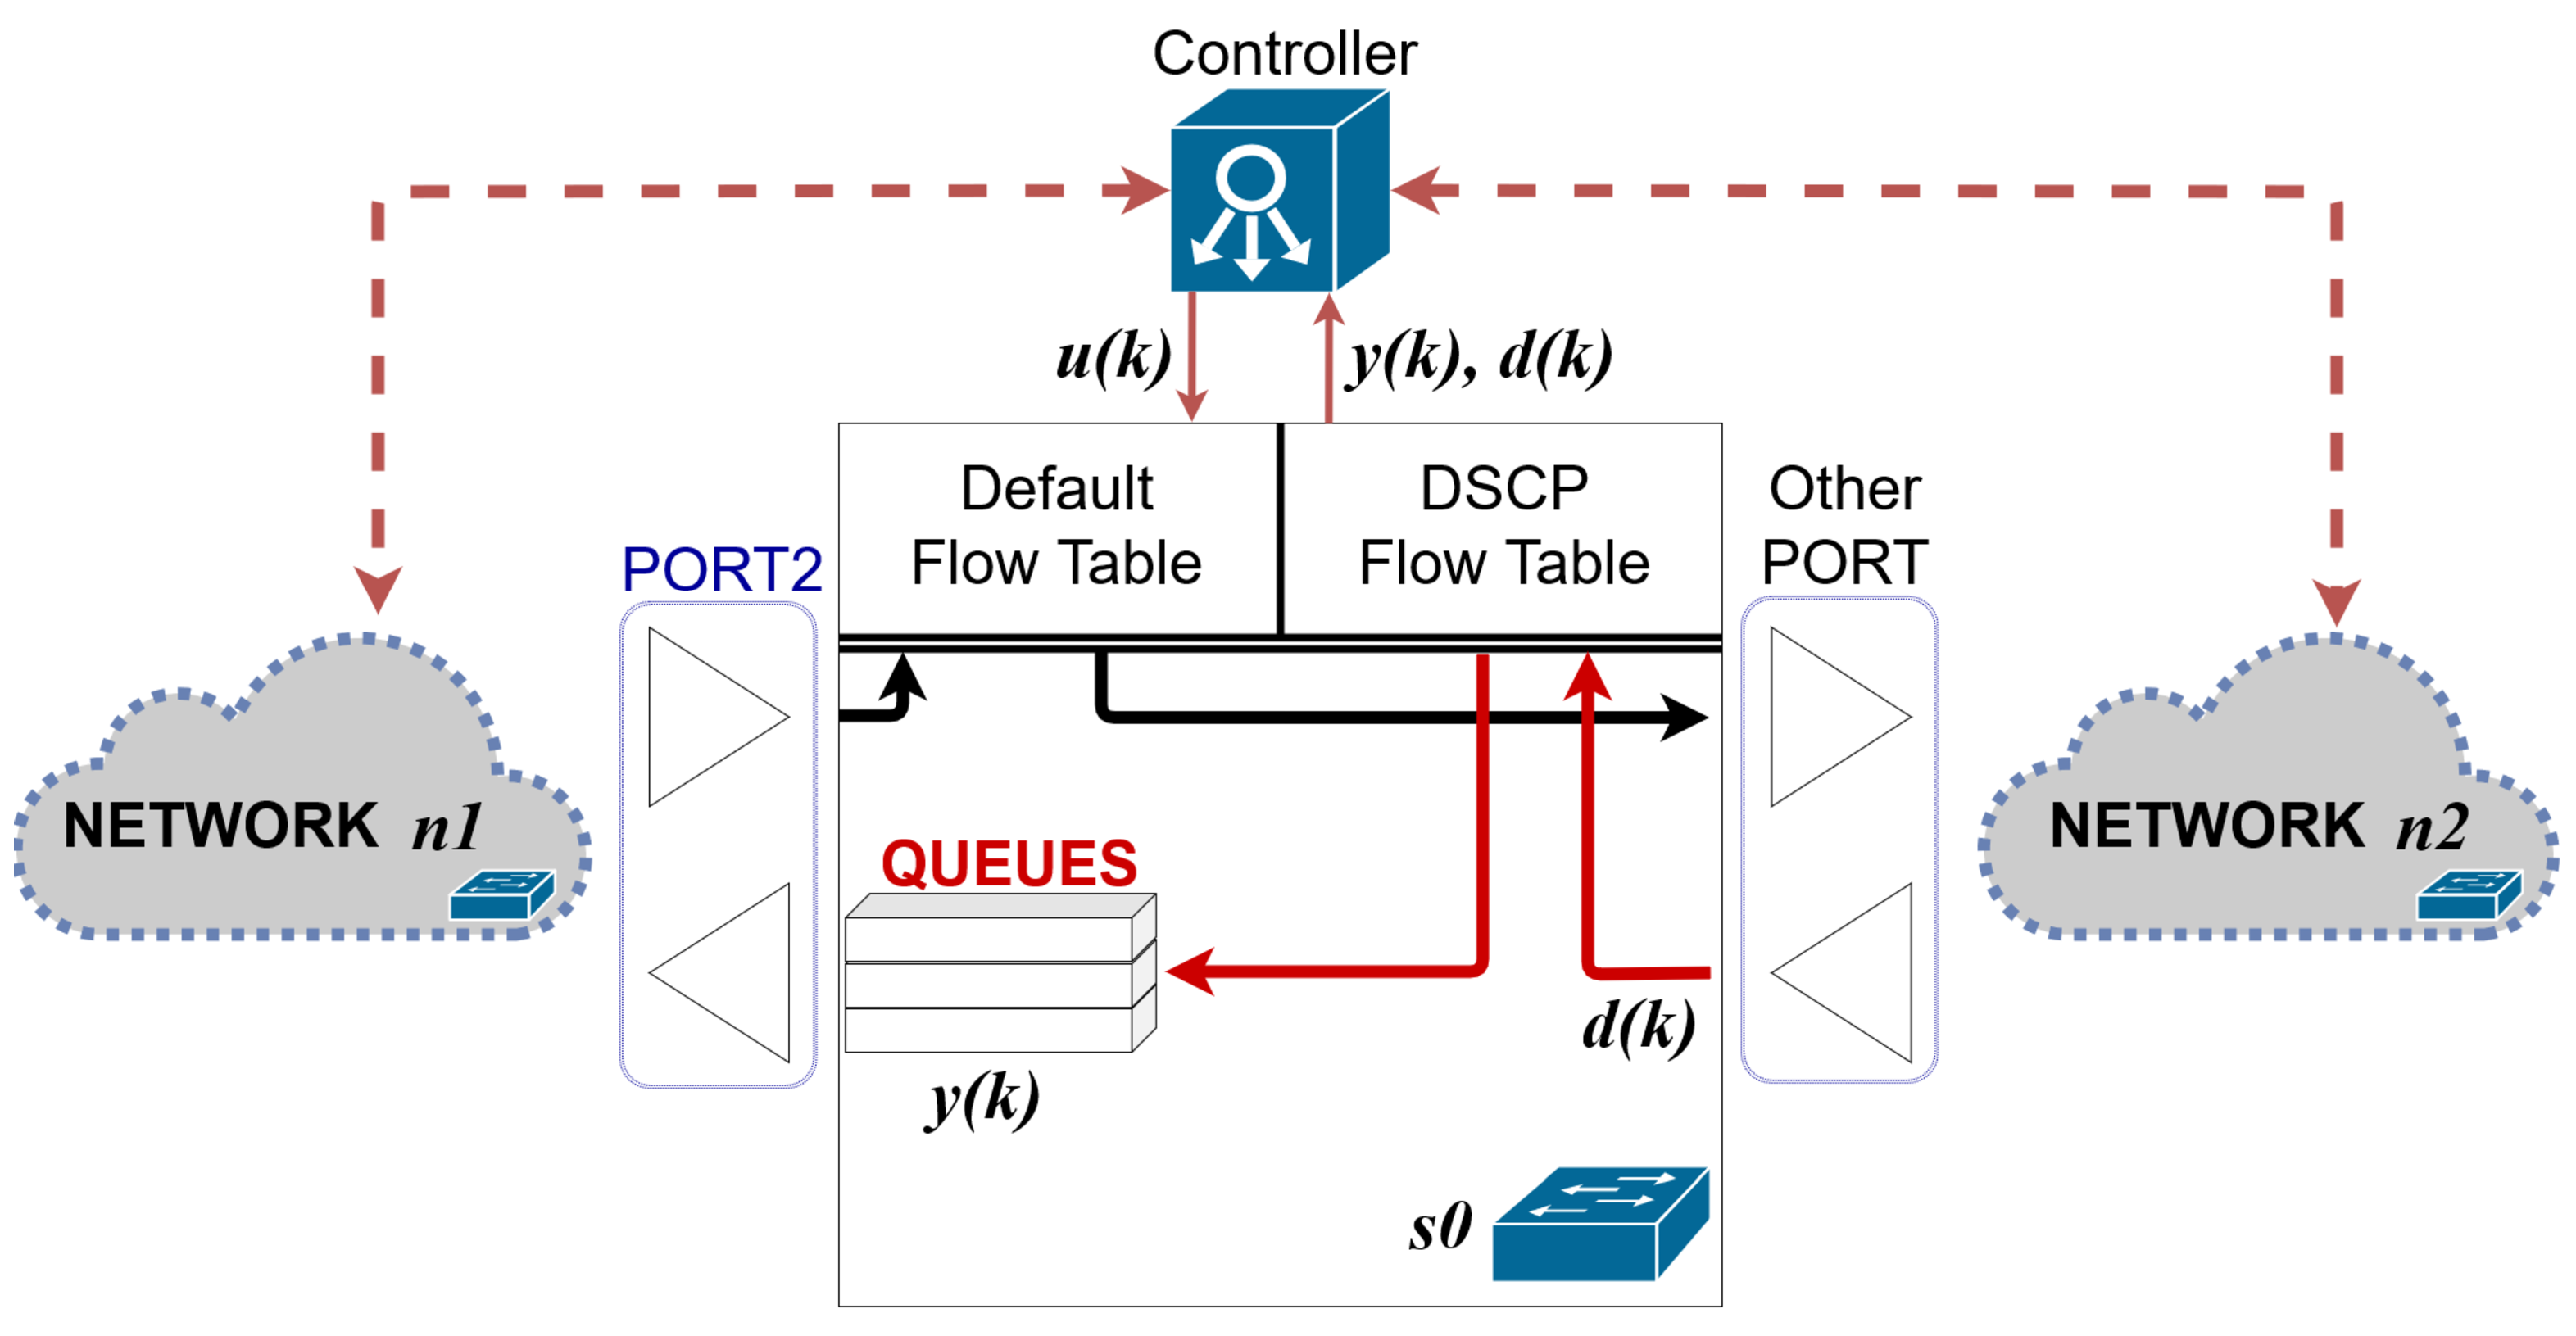
\includegraphics[keepaspectratio,width=\columnwidth]{figure/SDN_net_EPS.eps}
	\caption{Mininet emulated network architecture.}
	\label{fig:{Network}}
\end{figure}
%\begin{figure}[tb!]
%	\centering
%	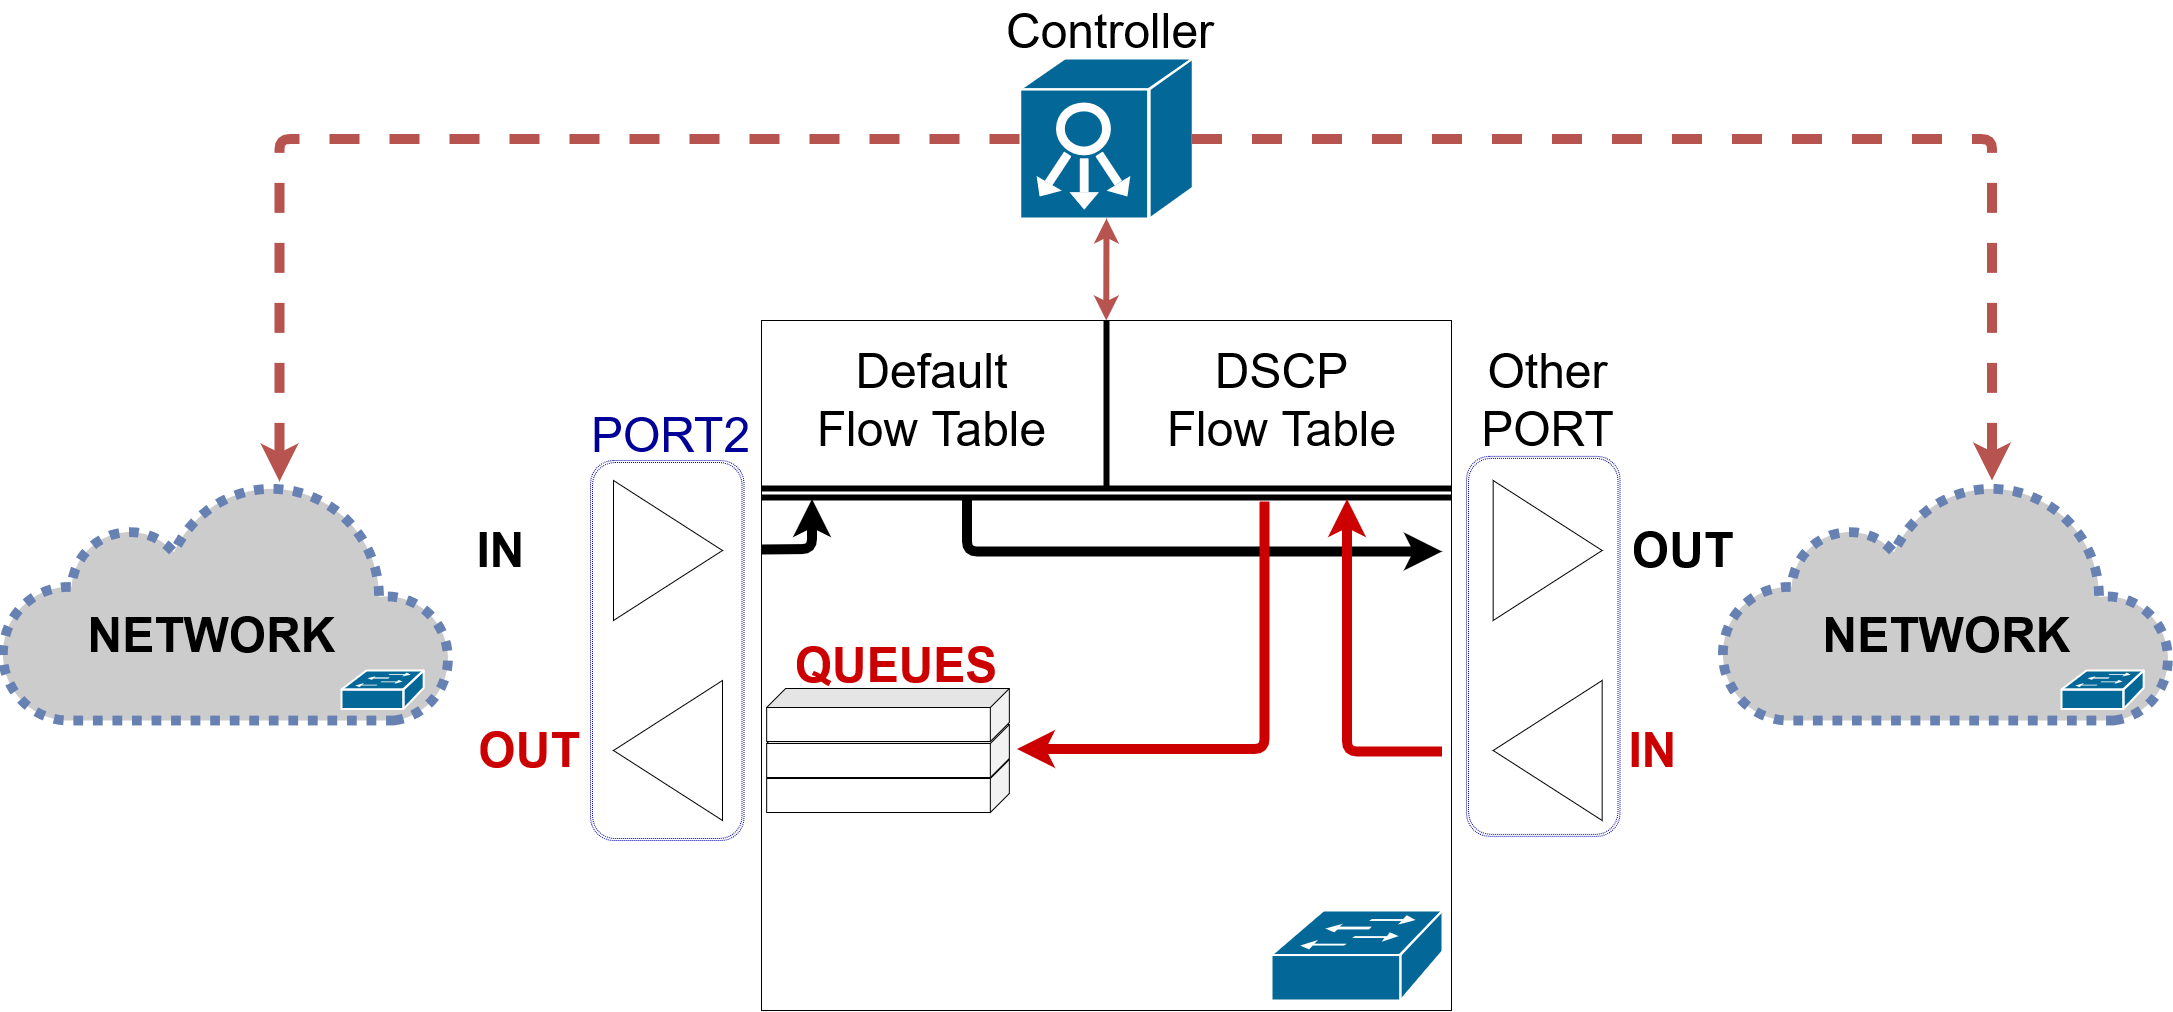
\includegraphics[width=13cm]{figure/SDN_net_LAST.png}
%	\caption{Simulated Network inside Mininet environment.}
%	\label{fig:{Network}}
%\end{figure}

For the purposes of this work, various network configurations were tested. Since similar results has been obtained on all configurations, it is possible to consider the generic case as the architecture in Figure \ref{fig:{Network}}, which aims to represent a portion of a larger network where a bottleneck occurs. More precisely, we consider a switch $s0$ with one input port and one output port, and a remote controller \cite{OVS, RYU} that dynamically manages the configuration of the queues of $s0$. The input of $s0$ is fed with an instance of D-ITG generating stochastic traffic, whose mean value follows the pattern of a real data set (where packets are differentiated by their ToS - Type of Service - priority index) extracted from two days logs of a router of a large service provider network. Namely, the original real data set contains traffic of a real network incoming from a source geographic area and terminating in a destination geographic area, and is divided for each value of Differentiated Services Code Point (DSCP) with a sampling time of 5 minutes \cite{Baker1998, Babiarz2006}. We recall that DSCP is the modern definition of the Type of Service (ToS) field, in which the first 6 bits are the Differentiated Services field that are in common with ToS field, and the last 2 bits regard explicit congestion notification. The ToS field can specify the priority of a datagram and the request for a low delay addressing, a high throughput or a high reliability service. Following the implementation of many national service provider networks (see e.g. \cite{Notiziario}), we partition the 8 different values of the DSCP in three classes: the \textit{Default} class (DSCPs $0,1,3$), the \textit{Premium} (DSCPs $2,4,6,7$), and the \textit{Gold} class (DSCP $5$): to each class we will assign a single queue, associated with a different priority.

%Traffic generation is entrusted to the D-ITG generator which uses informations inside a database created from a real measure that contains the number of packets transmitted and received by a switch. The database fields has been divided for each type of Differentiated Services Code Point (DSCP) with a sampling time of 5 minutes \cite{Baker1998, Babiarz2006}. DSCP is the modern definition of the Type of Service (ToS) field in which the first 6 bits are the Differentiated Services field that are in common with ToS field, and the last 2 bits are the explicit congestion notification. The ToS field can specify the priority of a datagram and the request for a low delay addressing, a high throughput or a high reliability service. Depending on the ToS values, a packet could be placed in a high priority exit queue, or follow a route with latency, throughput and the appropriate reliability for the request.


Using D-ITG Sender and Receiver SW modules it has been possible to establish a connection between networks n1 and n2. In particular, 16 ITG modules have been initialized: 8 for each network, and within each network one for each DSCP index. These modules handle the sampling time interval (5 minutes), the inter-departure time stochastic distribution associated with the packet rate, the packet size stochastic distribution, the IP and port destinations, and the DSCP index. Regarding the controller SW module we used Ryu, which provides software components with well defined Application Programming Interfaces (API) that give the possibility to easily create new network management and control applications. Ryu supports various protocols for managing network devices, such as OpenFlow, Netconf, OF-config, etc. About OF, Ryu supports fully 1.0, 1.2, 1.3, 1.4, 1.5 and Nicira Extensions. For our test-bed the 1.3 version has been chosen. In particular, APIs were used for queue control and counter recovery from the switches \cite{ofctlrest,QoS}. The feedback information collected for the purposes of this work are the descriptions of switches, ports and queues, the number of packets received and transmitted on each port of a switch, the packets passing through the flow tables, the packet rate values of each queue and the packets transmitted by each single queue. In summary, the variables associated to the traffic and control signals in our closed-loop architecture are as follows:

\begin{itemize}
	\item $d(k)\in\Real^{10}$ is a measurable disturbance vector, i.e. representing variables we cannot control. The first 8 components $d_1(k),\ldots,d_8(k)$ consist of the number of packets incoming in the switch $s0$ differentiated with respect to the 8 different values of the DSCPs. $d_9(k)$ and $d_{10}(k)$ are proxy variables, i.e. the hours and minutes of the day, which are very useful to the predictive model since traffic dynamics are tightly correlated with them, e.g. they are substantially different between night and day;
	\item $y(k)\in\Real^{3}$ is the measured output vector, i.e. the variables we want to regulate. They consist of the number of packets outgoing from switch $s0$ differentiated with respect to the corresponding service class: $y_1(k)$ is the Default Queue output, $y_2(k)$ is the Premium Queue output and $y_3(k)$ is the Gold Queue output;
	\item $u(k)\in\Real^{3}$ is the control input vector. Each component corresponds to the queue configuration of each service class: $u_1(k)$ is the Default Queue configuration, i.e. the maximum admitted bandwidth; $u_2(k)$ is the Premium Queue configuration, i.e. the maximum admitted bandwidth; $u_3(k)$ is the Gold Queue configuration, i.e. the minimum admitted bandwidth;
\end{itemize}

\begin{figure}[tb!]
	\centering
	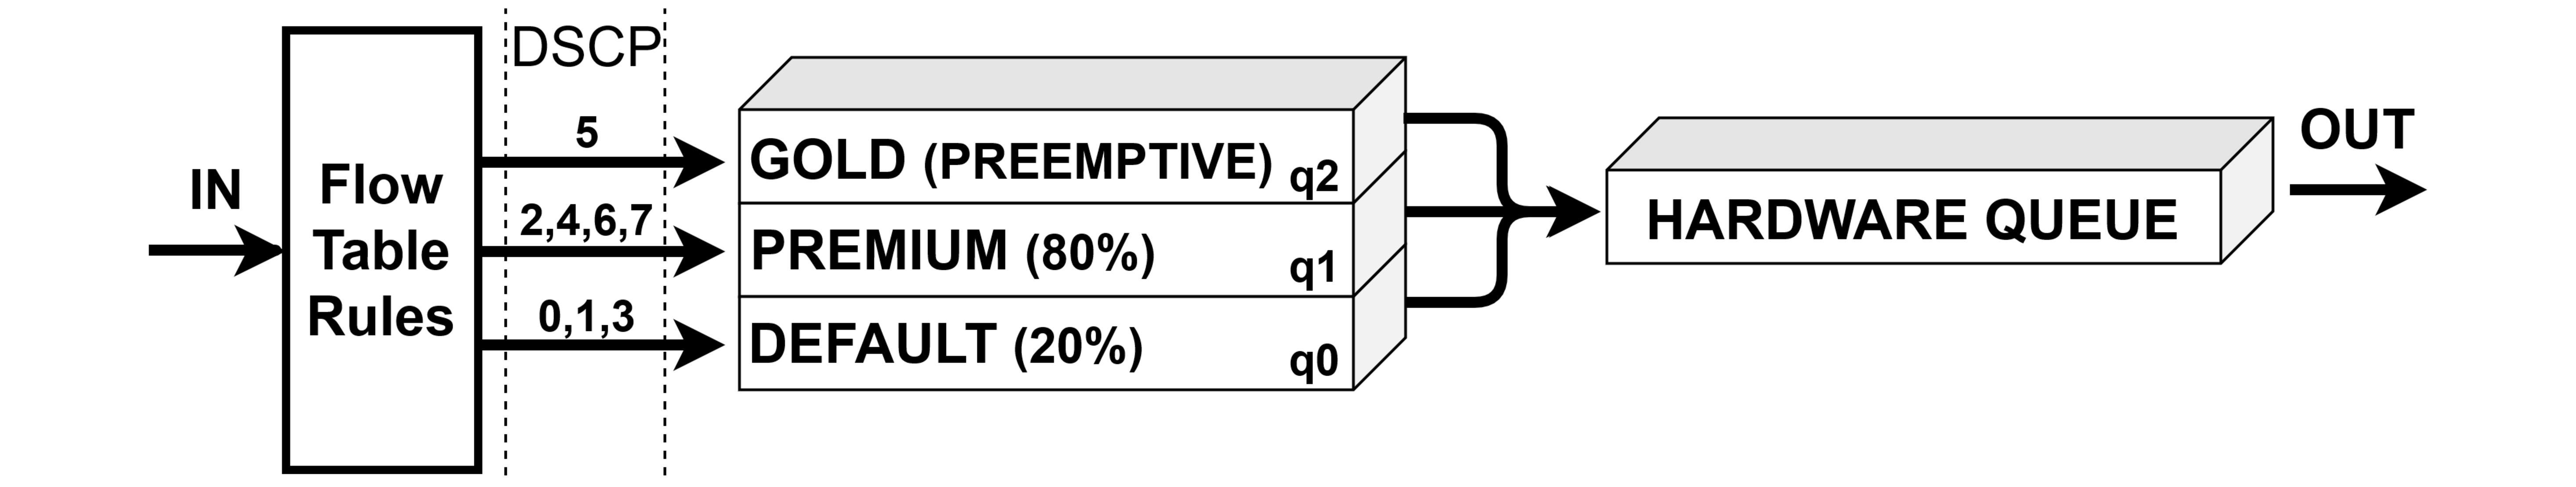
\includegraphics[keepaspectratio,width=\columnwidth]{figure/QUEUE.eps}
%	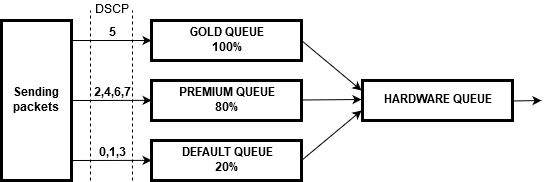
\includegraphics[keepaspectratio,width=12cm]{figure/queue.png}
	\caption{Static queues rate with routed packets relative to DSCP.}
	\label{fig:{queue}}
\end{figure}

In this work we first applied in our emulative scenario the static control of queues used in the Italian service provider network of \textit{Telecom Italia} \cite{Notiziario}, which is depicted in Figure \ref{fig:{queue}}. To this aim we defined 3 queues in $s0$ and configured the queues as follows: packets with the DSCP values 0, 1 and 3 (Default queue) are routed via queue 0, with maximum rate $u_1(k) = 20 \textit{MB/s}, \forall k$; the packets with values 2, 4, 6 and 7 (Premium queue) are routed on queue 1, with maximum rate $u_2(k) = 80 \textit{MB/s}, \forall k$; the packets with value 5 (Gold queue) are routed on queue 2, with minimum rate $u_3(k) = 100 \textit{MB/s}, \forall k$. To obtain this prioritization it has also been necessary to set the flow tables of $s0$ to discriminate incoming packets based on the DSCP value and the destination IP address, and re-route them to the desired queue. Also, to obtain a bottleneck situation in $s0$, we have chosen the bandwidth of the output port of switch $s0$ at 100 \textit{MB/s}. Using this configuration queue 2 uses the maximum capacity of the port to forward packets with preemptive priority, while the other two queues use the remaining bandwidth from 0 \textit{MB/s} to the specified maximum bandwidth based on needs.
%As formally defined later in Section \ref{secSwitchedModeling}, the packets sent by the queues will be collected in the state vector to be controlled $x(k)\in\mathbf{R}^3,\ \forall k$,  while the bandwidth associated to the queues will compose the control variables vector $u(k)\in\mathbf{R}^3,\ \forall k$.
To instantiate the chosen topology in Mininet it has been necessary to run the \ref{Topology} code from the Ubuntu command line with the following text:\\
\Blackline{ sudo python Topology\textunderscore qos.py}
In this script all network devices (remote controller, switches and hosts), their attributes and their connections are defined. Furthermore this script is also responsible for the traffic generated between hosts thanks to the function defined within the \ref{ditg} code that is iteratively used every five minutes to read the provided real data traffic database and generate the synthetic traffic inside the network. In lines $49$ to $53$ of \ref{Topology} code Mininet adds an external controller, Ryu in our case, to specified IP address and port. Obviously it is necessary that the controller is already instantiated before launching the network topology, and it is possible to do this through the following command:
\Blackline{ ryu run main\textunderscore controller\textunderscore TOS.py rest\textunderscore qos.py rest\textunderscore conf\textunderscore switch.py ofctl\textunderscore rest.py}
This command executes several scripts, the first one (\ref{main_controller_TOS}) is the Ryu controller which invokes additional functions designed for saving network information and setting queue bandwidths (from \ref{datapath_monitor_TOS} to \ref{qos_simple_switch_13}). The remaining scripts are all the rest APIs required for these features to work properly (\ref{ofctl_rest}, \ref{rest_conf_switch} and \ref{rest_qos} codes).

As we will see in Section \ref{secExpRes}, using static priority control the queues will not be able to send all the packets incoming from network $n1$, and a dramatic amount of packets will be lost. This motivates the application of optimization techniques, which are enabled by the predictive models derived using the methodology described in section \ref{secSwitchedModeling}.

\section{Regression Trees and Random Forest based models for MPC}\label{secSwitchedModeling}
In this section a methodology to apply the results proposed in \cite{SmarraADHS2018,smarraNAHS2020} is illustrated, to identify, starting from a set of collected historical data $ \mathcal{D}=\{y(k),u(k),d(k)\}_{k = 0}^{\ell} $ (generated as described in the previous section), a switching ARX model of the input-output behavior of the traffic flow in a switch of a SDN network as follows:
%The aim of such predictive model is to enable the direct and computationally efficient implementation of Model Predictive Control for bandwidth and packet losses optimisation.
%\small
\begin{equation}\label{eqIdentifiedModelNSARX}
x(k+j+1) =	A'_{\sigma_j(x(k),d(k))} x(k) + \sum_{\alpha = 0}^{j}B'_{\sigma_{j}(x(k),d(k)),\alpha} u(k+\alpha) + f'_{\sigma_j(x(k),d(k))},
\end{equation}
%\normalsize
\noindent $j = 0,\ldots, N-1$, where $x(k) \doteq [y^\top(k)\ \cdots\ y^\top(k-\delta_y)\ u^\top(k-1)\ \cdots\ u^\top(k-\delta_u)]^\top\in\Real^{n_x}$ is an extended state to characterize a switching ARX model, with $x_\iota(k) \doteq [y_\iota(k)\ \cdots\ y_\iota(k-\delta_y)\ u^\top(k-1)\ \cdots\ u^\top(k-\delta_u)]^\top\in\Real^{\delta_y+1+3\delta_u}$, $\iota = 1,2,3$, $N$ is the chosen future predictive horizon, and  $\sigma_j : \mathbb{R}^{n_x+10} \to \mathcal M \subset \mathbb{N}$ is a switching signal that associates an operating mode in a finite set $\mathcal M$ to each pair $(x(k),d(k))$ and each prediction step $j$ of the horizon.
It is possible to directly use model \eqref{eqIdentifiedModelNSARX} to setup the following problem, which can be solved using standard Quadratic Programming (QP) solvers:\\
\begin{problem}\label{pbMPCSwitching}
%	\small
	\vspace{-0.3cm}
	\begin{equation*}
		\begin{aligned}
			& \underset{u_0,\ldots,u_{N-1}}{\text{minimize}} & &  \sum_{j=0}^{N-1} \left(\left(x_{j+1}-x_{\mathrm{ref}}\right)^\top Q \left(x_{j+1}-x_{\mathrm{ref}}\right) + u^\top_{j} R u_{j}\right)\\
			& \text{subject to }            & &  x_{j+1} = A'_{\sigma_j(x_{0},d_{0})} x_0 + \sum_{\alpha = 0}^{j}B'_{\sigma_{j}(x_{0},d_{0}),\alpha} u_\alpha + f'_{\sigma_j(x_{0},d_{0})}\\       
			&                               & &  u_{j}   \in \mathcal{U}\\
			&                               & &  x_{0} = x(k), d_{0} = d(k)\\ 
			&                               & &  j = 0,\ldots,N-1.			\\
		\end{aligned}
		\vspace{0.1cm}
	\end{equation*}
%	\normalsize
\end{problem}
\noindent As it is well known \cite{borrelli2017predictive}, Problem \ref{pbMPCSwitching} is solved at each time step $k$ using QP to compute the optimal sequence $u^*_0,\ldots,u^*_{N-1}$, but only the first input is applied to the system, i.e. $u(k) = u^*_0$. Note that, for any prediction step $j$, $x_{j+1}$ only depends on the measurements $x_0=x(k),d_0=d(k)$ at time $k$, since they are the only available measurements at time-step $k$. 
%\subsection{Switching ARX Identification using RF}\label{secSARX}

\subsection{RT and RF background}
Let us consider a dataset $\{y(k),x_1(k),\ldots,x_\eta(k)\}_{k=0}^\ell$, with $y,x_1,\ldots,x_\eta\in\mathbb{R}$. Let us suppose  to estimate, using Regression Trees, the prediction of the (response) variable $y(k)$ using the values of predictor variables $x_1(k),\ldots,x_\eta(k)$. The CART algorithm \cite{BreimanCART2017} creates a RT structure via optimal partition of the dataset. It solves a Least Square problem by optimally choosing recursively a variable to split and a corresponding splitting point. After several steps the algorithm converges to the optimal solution, and the dataset is partitioned in hyper-rectangular regions (the leaves of the tree) $R_1, R_2,\cdots, R_\nu$. In each partition $y(k)$ is estimated with a different constant $\hat y_i\, i=1,\ldots,\nu,$ given by the average of the samples of $y(k)$ falling in $R_i$, i.e.

\begin{equation}\label{eqAverageResponseRT}
\hat y_{i} = \frac{\sum\limits_{\{k|(x_1(k),\ldots, x_\eta(k)) \in R_i\}}y(k)}{|R_i|}
\end{equation}


\noindent Random Forests \cite{BreimanML2001} are instead an averaging method that exploits a combination of tree predictors such that each tree depends on the values of a random vector sampled independently and with the same distribution for all trees in the forest. The output prediction is given by averaging the predictions provided by all trees in the forest. It is possible to show that the error introduced by the forests quickly and almost surely converges to a limit as the number of trees in the forest becomes large. Such error also depends on the strength of the individual trees in the forest and the correlation between them. Thus, due to the Law of Large Numbers, Random Forests (differently from Regression Trees) do not suffer much variance and overfitting problems. For more details the reader is refered to \cite{BreimanCART2017,BreimanML2001}.

\subsection{Switching ARX (SARX) model identification via RT} To derive a model as in \eqref{eqIdentifiedModelNSARX}, a new dataset $\X= \{x(k),u(k),d(k)\}_{k = 0}^{\ell}$ has to be defined starting from $\D$. In order to apply MPC it is needed, for each component of $y(k)$, a model that can predict system's dynamics over a horizon of length $N$. The idea is to create $3 N$ predictive trees $\{\mathcal{T}_{\iota,j}\},\ \iota=1,2,3,\ j=0,\ldots,N-1$, each one to predict the 3 outputs components of the system over the $N$ steps of the horizon. To create the tree structure, the RT algorithm (CART) partitions the dataset $\X$ into regions $\X_i$, such that $\biguplus \X_i = \X$, and assigns to each region a constant value given by the average of the output values of the samples that ended up in that leaf. In run-time, once the trees are created, and given a real-time measurement $(x(k), u(k), d(k))$ belonging to leaf $i$, the CART algorithm provides as a prediction the averaged value associated to the leaf as in \eqref{eqAverageResponseRT}. However, since the prediction provided by the RT is a constant value, it cannot be used to setup an MPC problem, thus the learning procedure needs to be modified to identify a modeling framework as in \eqref{eqIdentifiedModelN}. To this end, $\X$ is partitioned in two disjoint sets $\mathcal{X}_c = \{u(k)\}_{k=0}^{\ell}$ of data associated to the control variables, and $\mathcal{X}_{nc} = \{(x(k), d(k))\}_{k=0}^{\ell}$ of data associated to remaining variables, and then apply the CART algorithm only on $\mathcal{X}_{nc}$ (this is to avoid that the MPC problem turns out into a Mixed Integer Quadratic Program, see \cite{SmarraADHS2018,smarraNAHS2020} for details); thus, $3 N$ RTs $\{\mathcal{T}_{\iota,j}\}$ have been created, each constructed to predict the variable $y_\iota(k+j+1)$, and consequently $x_\iota(k+j+1)$. In particular, it is associated to each leaf $\iota,i_j$, corresponding to the partition  $\mathcal{X}_{nc,\iota,i_j}$, of each tree $\mathcal{T}_{\iota,j}$ the following affine model is associated

%\small
%
\begin{equation}\label{eqLTIleavesSinglState}
	x_\iota(k+j+1) = A'_{\iota,i_j}x(k) + \sum_{\alpha = 0}^{j}{B'_{\iota,i_j,\alpha}u(k+\alpha)} + f'_{\iota,i_j},
\end{equation}
%\normalsize
%\small
\begin{equation}\label{eqLeafModel}
\begin{aligned}
A'_{\iota,i_j} =& \left[\begin{array}{cccccccccc}
a_1       & a_2       & \cdots & a_{\delta_y } & a_{\delta_y + 1} & b_{\delta_y + 2} & \cdots & b_{\delta_y + 1+ 3(\delta_u-1)} & \cdots & b_{\delta_y + 1 + 3\delta_u} \\
1         & 0         & \cdots & 0             & 0                & 0                & \cdots & 0                               & \cdots & 0                            \\
\vdots    & \vdots    & \ddots & \vdots        & \vdots           & 0                & \cdots & 0                               & \cdots & 0                            \\
0         & 0         & \cdots & 1             & 0                & 0                & \cdots & 0                               & \cdots & 0                            \\
0         & 0         & \cdots & 0             & 0                & 0                & \cdots & 0                               & \cdots & 0                            \\
0         & 0         & \cdots & 0             & 0                & 0                & \cdots & 0                               & \cdots & 0                            \\
0         & 0         & \cdots & 0             & 0                & 0                & \cdots & 0                               & \cdots & 0                            \\
0         & 0         & \cdots & 0             & 0                & 1                & \cdots & 0                               & \cdots & 0                            \\
\vdots    & \vdots    & \ddots & \vdots        & \vdots           & \vdots           & \ddots & \vdots                          & \ddots & \vdots                       \\
0         & 0         & \cdots & 0             & 0                & 0                & \cdots & 1                               & \cdots & 0                            \\

\end{array}\right],\\
B'_{\iota,i_j,\alpha} = & \left[\begin{array}{ccc}
b_{1,\alpha} & b_{2,\alpha} & b_{3,\alpha}\\
0            & 0            & 0            \\
\vdots       & \vdots       & \vdots \\
0            & 0            & 0            \\   
0            & 0            & 0            \\  
0            & 0            & 0            \\  
0            & 0            & 0            \\  
0            & 0            & 0            \\  
\vdots       & \vdots       & \vdots            \\   
0            & 0            & 0            \\   
\end{array}\right],\ \alpha<j,\ 
B'_{\iota,i_j,j} =  \left[\begin{array}{ccc}
b_{1,\alpha} & b_{2,\alpha} & b_{3,\alpha}\\
0            & 0            & 0            \\
\vdots       & \vdots       & \vdots \\
0            & 0            & 0            \\   
1            & 0            & 0            \\  
0            & 1            & 0            \\  
0            & 0            & 1            \\  
0            & 0            & 0            \\  
\vdots       & \vdots       & \vdots            \\   
0            & 0            & 0            \\   
\end{array}\right],\ 
f'_{\iota,i_j} = \left[\begin{array}{ccccc}
f      \\	0 \\ \vdots \\ 0 \\ 0 \\ 0 \\ 0 \\ 0 \\ \vdots \\ 0      
\end{array}\right],
\end{aligned}
\end{equation}
%\normalsize

\noindent where the coefficients of matrices $A'_{\iota,i_j}$, $B'_{\iota,i_j,\alpha}$ and $f'_{\iota,i_j}$ are obtained in each leaf $\iota,i_j$ by fitting the corresponding set of samples solving the following Least Squares with inequality constraints problem:

\begin{problem}\label{pbLeastSquareProblem}
%	\small
	\begin{alignat}{2}
		& \nonumber \underset{\xi_{\iota,i_j}}{\text{minimize}} & &  \parallel \Lambda_{\iota,i_j} \xi_{\iota,i_j}  - \lambda_{\iota,i_j} \parallel_2^2   		 \\
		& \text{subject to }    \nonumber            & &  f_\mathrm{min} \leq f \leq f_\mathrm{max}    										  					 \\
		&                  					    	 & &  a_\mathrm{min} \leq a_{\jmath} \leq a_\mathrm{max}\label{eqInequalityConstraints} \\
		& 	                    \nonumber			 & &  b_\mathrm{min} \leq b_{\iota,\alpha} \leq b_\mathrm{max},
	\end{alignat}
%	\normalsize
\end{problem}

\noindent where $\xi_{\iota,i_j}$, $\lambda_{\iota,i_j}$, and $\Lambda_{\iota,i_j}$ contain respectively the parameters of matrices in \eqref{eqLeafModel}, the predictions $x_\iota(k+j+1)$, and the current measurements of $x(k)$ and $u(k+\alpha)$. Linear inequalities \eqref{eqInequalityConstraints} are used to constrain elements in $\xi_{\iota,i_j}$ to take into account physical system constraints and improve prediction accuracy.
Model \eqref{eqLTIleavesSinglState} can be easily compacted in the following form taking into account all the states $\iota=1,2,3$:
%\small
\begin{equation}\label{eqLTIleavesCompact}
x(k+j+1) = A'_{i_j}x(k) + \sum_{\alpha = 0}^{j}{B'_{i_j,\alpha}u(k+\alpha)} + f'_{i_j}.
\end{equation}
%\normalsize
\noindent In particular, with the specific choice of $\delta_u = 0$ model \eqref{eqIdentifiedModelNSARX} can be rewritten in the following state-space formulation
%\small
\begin{equation}\label{eqIdentifiedModelN}
x(k+j+1) =	A_{\sigma_j(x(k),\bold{u^-}(k),d(k))} x(k+j) + B_{\sigma_j(x(k),\bold{u^-}(k),d(k))} u(k+j) + f_{\sigma_j(x(k),\bold{u^-}(k),d(k))},
\end{equation}
%\normalsize
where $\bold{u^-}(k) = [u^\top(k-1)\ \cdots\ u^\top(k-\delta)]^\top$ is the vector with the regressive terms of the input used to only grow the trees, and  $\sigma_j : \mathbb{R}^{3(\delta_y+1)+3\delta+10} \to \mathcal M \subset \mathbb{N}$.
%\noindent In particular, as anticipated in the problem formulation, with the specific choice of $\delta_u = 0$ matrices $A'_{\iota,i_j}$ in \eqref{eqLeafModel} modify as follows:
%
%\small
%\begin{equation}\label{eqLeafModelDelta_u=0}
%	\begin{aligned}
%		A'_{\iota,i_j} =& \left[\begin{array}{ccccc}
%			a_1       & a_2       & \cdots & a_{\delta_y } & a_{\delta_y + 1} \\
%			1         & 0         & \cdots & 0                         & 0     \\
%			\vdots    & \vdots    & \ddots & \vdots                    & \vdots     \\
%			0         & 0         & \cdots & 1                         & 0     
%		\end{array}\right]\\
%		B'_{\iota,i_j,\alpha} = & \left[\begin{array}{ccccc}
%			b_{1,\alpha} & 0 & \cdots & 0 & 0\\
%			b_{2,\alpha} & 0 & \cdots & 0 & 0           \\
%			b_{3,\alpha} & 0 & \cdots & 0 & 0           \\   
%		\end{array}\right]^\top\\
%				f'_{\iota,i_j} = &\left[\begin{array}{ccccc}
%		f      &	0 & \cdots & 0 & 0      
%		\end{array}\right]^\top.
%	\end{aligned}
%\end{equation}
%%\normalsize
Thanks to this new formulation the following proposition shows that model \eqref{eqLTIleavesCompact} is equivalent to model \eqref{eqIdentifiedModelN} for any initial condition, any switching signal and any control sequence.
\begin{proposition}\label{propSwitchingSystem}\cite{smarraNAHS2020}
	Let $A'_{i_j}$, $B'_{i_j,\alpha}$ and $f'_{i_j}$, $\alpha=0,\ldots,j$, $j=0,\ldots,N-1$, be given. If $A'_{i_j}$ is invertible for $j=0,\ldots,N-1$, then there exists a model in the form
	\vspace{-0.2cm}
%	\small
	\begin{equation*}
	\bar x({k+j+1}) = A_{\sigma_j(\bar x(k),\bold{u^-}(k), d(k))} \bar x({k+j})+B_{\sigma_j(\bar x(k),\bold{u^-}(k), d(k))} u({k+j})+ f_{\sigma_j(\bar x(k),\bold{u^-}(k), d(k))}	
	\end{equation*}
%	\normalsize
	such that for any initial condition $\bar x(k) = x(k) = x_k$, any switching sequence $i_0, \ldots, i_{N-1}$ and any control sequence $u(k),\ldots,u(k+N-1)$, then $\bar x(k+j+1) = x(k+j+1),\ \forall j=0,\ldots,N-1$.
\end{proposition}

As discussed in \cite{smarraNAHS2020}, from experimental findings it is possible to notice that the contribution in terms of model accuracy introduced by the choice of $\delta_u = 0$ is negligible, since previous control inputs are already considered in the tree structure choosing $\delta > 0$. Thus, in the rest of the thesis it will be considered $\delta_u = 0$ and $\delta > 0$, i.e. only the regressive terms of the input in the tree structure learning will be used and not in the state definition.

\subsection{SARX model identification via RF} RF-based models can be constructed exploiting the RT-based formulation: in particular, let us consider $3 N$ RFs $\mathcal{F}_{\iota,j}$, $\iota = 1,2,3,\ j = 0,\ldots,N-1$. 
For each tree $\mathcal{T}^{\mathcal{F}_{\iota,j}}_\tau$ of the forest $\mathcal{F}_{\iota,j}$, it is possible to estimate the coefficients $a_*$, $b_*$ and $f$ in \eqref{eqLeafModel} for each leaf $\iota,j,i_\tau$, i.e. $\tilde\xi_{\iota,j,i_\tau}$, solving Problem \ref{pbLeastSquareProblem}.
With a small abuse of notation, let us indicate by $|\mathcal{F}_{\iota,j}|$ the number of trees in the forest ${\iota,j}$. 
Then $\forall \iota,j$, the parameters to build matrices in \eqref{eqLTIleaves} can be obtained by averaging parameters $a_*$, $b_*$ and $f$, $\forall \tau = 1,\ldots,|\mathcal{F}_{\iota,j}|$, i.e.
%\small
\begin{equation}\label{eqAverageRF}
\tilde\xi_{\iota,j} = \frac{\sum\limits_{\tau=1}^{|\F_{\iota,j}|}\tilde\xi_{\iota,j,i_\tau}}{|\F_{\iota,j}|},
\end{equation}
%\normalsize
over all the trees of forest $\F_{\iota,j}$. At this point, starting from \eqref{eqLTIleavesSinglState}, it can be easily construct the following model, as in \eqref{eqLTIleavesCompact} to be used in the MPC formulation by combining for $\iota=1,2,3$ the matrices in \eqref{eqLeafModel} coming either from the RTs or from the RFs:
%\small
\begin{equation}\label{eqLTIleaves}
	x(k+j+1) = A'_{i_j}x(k) + \sum_{\alpha = 0}^{j}{B'_{i_j,\alpha}u(k+\alpha)} + f'_{i_j}.
\end{equation}
%\normalsize

%====================================================================================================

\subsection{MPC problem formulation.} Model \eqref{eqLTIleaves} is used to formalize Problem \ref{pbMPCSwitching} according to the SDN priority queueing problem:
\begin{problem}\label{pbMPC}

	\begin{equation*}
		\begin{aligned}
			& \underset{\bold u}
			{\text{minimize}}               & &  \sum_{j=0}^{N-1} \Big[(x_{j+1}-x_{\mathrm{ref},j})^\top Q (x_{j+1}-x_{\mathrm{ref},j}) + u^\top_{j} R u_{j}\Big]   \\
			& \text{subject to}             & &  x_{j+1}  =   A_{\sigma_j(k)} x_{j}+B_{\sigma_j(k)}  u_j+f_{\sigma_j(k)} \\
			&								& &  \Delta u_\iota^\mathrm{min} \leq u_{\iota,j} - u_{\iota,j-1} \leq \Delta u_\iota^\mathrm{max}             \\
			&								& &  u_\iota^\mathrm{min} \leq u_{\iota,j} \leq u_\iota^\mathrm{max}             \\
			&                               & &  u_{1,j} + u_{2,j} \leq 100			          		\\
			&                               & &  x_0 = x(k),\ \bold u^-_{0} = [u^\top(-1)\ \cdots\ u^\top(-\delta)]^\top,\ d_0 = d(k),\\
			&								& &  j = 0,\ldots,N-1,\ \iota = 1,2,3,                                 
		\end{aligned}
	\end{equation*}
%	\normalsize
\end{problem}
\noindent where $\sigma_j(k) = \sigma_j(x(k),\bold{u^-}(k),d(k))$ (with a slight abuse of notation), $u_{\iota,j}$ is the $\iota^{th}$ component of the input $u$ at time $k+j$; $\Delta u_\iota^\mathrm{min}$ and $\Delta u_\iota^\mathrm{max}$ are used to limit large variations on the inputs in 2 consecutive steps, in order to avoid that the queues drastically set to the minimum value and thus potentially increase packet losses during the next period; $u_\iota^\mathrm{min}$ and $u_\iota^\mathrm{max}$ define the bandwidth limits induced by the QoS requirements of the corresponding priority class. At each time step $k$ the measurements of the variables in $\X_{nc}$ are collected, select the current matrices of \eqref{eqLTIleaves} narrowing down the leaves of the trees, for $j = 0,\ldots,N-1$, solve Problem \eqref{pbMPC}, and finally apply only the first input of the optimal sequence $\bold u^*$ found, i.e. $u(k) = u_0^*$.

%====================================================================================================

\subsection{Disturbance forecast} The knowledge at each time $k$ of the future input traffic $(d(k+1), \ldots, d(k+N-1))$ can greatly improve the MPC performance. However, while the future values of the proxy variables (hours and minutes) are clearly well known, the knowledge of the future values of the first 8 component of the disturbance, i.e. number of packets incoming in the switches for each DSCP index are unknown at the current instant $k$. To address this problem $8(N-1)$ RFs $\mathcal{F}^d_{\iota,j},\ \iota=1,\ldots,8,\ j = 0,\ldots,N-1$ have been built in order to provide a prediction $\hat d_\iota(k+j)$ of the 8 disturbance components $d_\iota(k+j)$ over the future time horizon: as widely illustrated in \cite{SmarraADHS2018,smarraNAHS2020} the technique previously described can be easily modified by appropriately redefining the dataset as $\mathcal{X} = \{(x(k), u(k), d(k),\ldots,d(k+N-1))\}_{k=1}^{\ell}$ for the training phase, and considering a switching signal in \eqref{eqIdentifiedModelN} given by $\sigma_j(k) = \sigma_j(x(k),\bold{u^-}(k),d(k),\hat d(k+1),\ldots,\hat d(k+j)), \forall j=0,\ldots,N-1$, i.e. also depending at time $k$ on the future input traffic.

%====================================================================================================
%====================================================================================================
\section{Simulation results}\label{secExpRes}
In this section simulation results of the application of the proposed approach to SDN Priority Queueing identification and control will be provided. Standard RFs are used to derive predictive models of the disturbance components $d_1(k),\ldots,d_8(k)$, i.e. the switch input differentiated for each DSCP index, and validate the accuracy. Then the validation of accuracy of the predictive model of the output variable $y(k)$ derived as illustrated in Section \ref{secSwitchedModeling} is shown: the predictive models (based on RTs and RFs) will be compared with Artificial Neural Networks, showing that RFs represent the ideal solution both in terms of prediction accuracy and computational complexity; then the effect of iterative dataset updates in the prediction accuracy is illustrated, both with and without prediction of the future disturbances. Finally the proposed predictive models will be used to setup a MPC problem (see Problem \ref{pbMPC}), and validate the control performance in terms of packet losses reduction and bandwidth saving, both with and without prediction of the future disturbances. It will also be shown, as expected, that using accurate predictive models and applying MPC provides dramatic reduction of packet losses and increase of bandwidth saving with respect to the static bandwidth allocation policy used in Service Provider Networks as described in Section \ref{sec:SDNNetSim}: even thought this result is not surprising, it is decided to quantify the gap to emphasize that much better performance can be obtained in real networks just collecting historical data and applying a controller that can be directly implemented using the accurate models of the proposed identification algorithm and Quadratic Programming solvers (which are well known to be very efficient).

In each of the aforementioned validations, 4 different predictive models have been exploited, using iteratively enriched data sets. More precisely, \textbf{OLD} is a predictive model identified with a data set of $5124$ samples, collected with a sampling time of $5$ minutes and obtained from network emulation with random values of the input $u(k)$; \textbf{1UP} is a predictive model identified with the \textbf{OLD} data set enriched with $3456$ new samples obtained from network emulation when applying closed-loop MPC to define the input $u(k)$; \textbf{2UP} is a predictive model identified with the \textbf{1UP} data set enriched with $3168$ new samples obtained from network emulation when applying closed-loop MPC to define the input $u(k)$; \textbf{3UP} is a predictive model identified with the \textbf{2UP} data set enriched with $6336$ new samples obtained from network emulation when applying closed-loop MPC to define the input $u(k)$. An independent data-set composed by $1684$ samples is used to validate the above models.
%Before running the identification algorithms, the dataset has been pre-processed checking if all measurements were coherent and if there were voids or data misalignments that could have distorted the model.
All simulations have been ran on a UDOO x86 Advanced with an Intel Braswell N3160 processor up to 2.24 GHz and 4 GB of RAM \cite{UDOO}.

\subsection {Disturbance predictive model validation} Having an accurate model of the variable $d(k)$ (i.e. the switch input differentiated for each DSCP index) can be helpful to improve the model identification performance as well as the reference input $x_\mathrm{ref}$ to follow in Problem \ref{pbMPC}. In this section we apply standard RF algorithms, with a regressive index of $15$ steps and $30$ trees for each forest, to obtain a predictive model of the disturbance over a predictive horizon of $N=5$ ($25$ minutes): this choice of $N$ has been taken considering the tradeoff between time complexity of the identification algorithm and the obtained identification accuracy. 

\begin{figure}[h!]
	\centering
	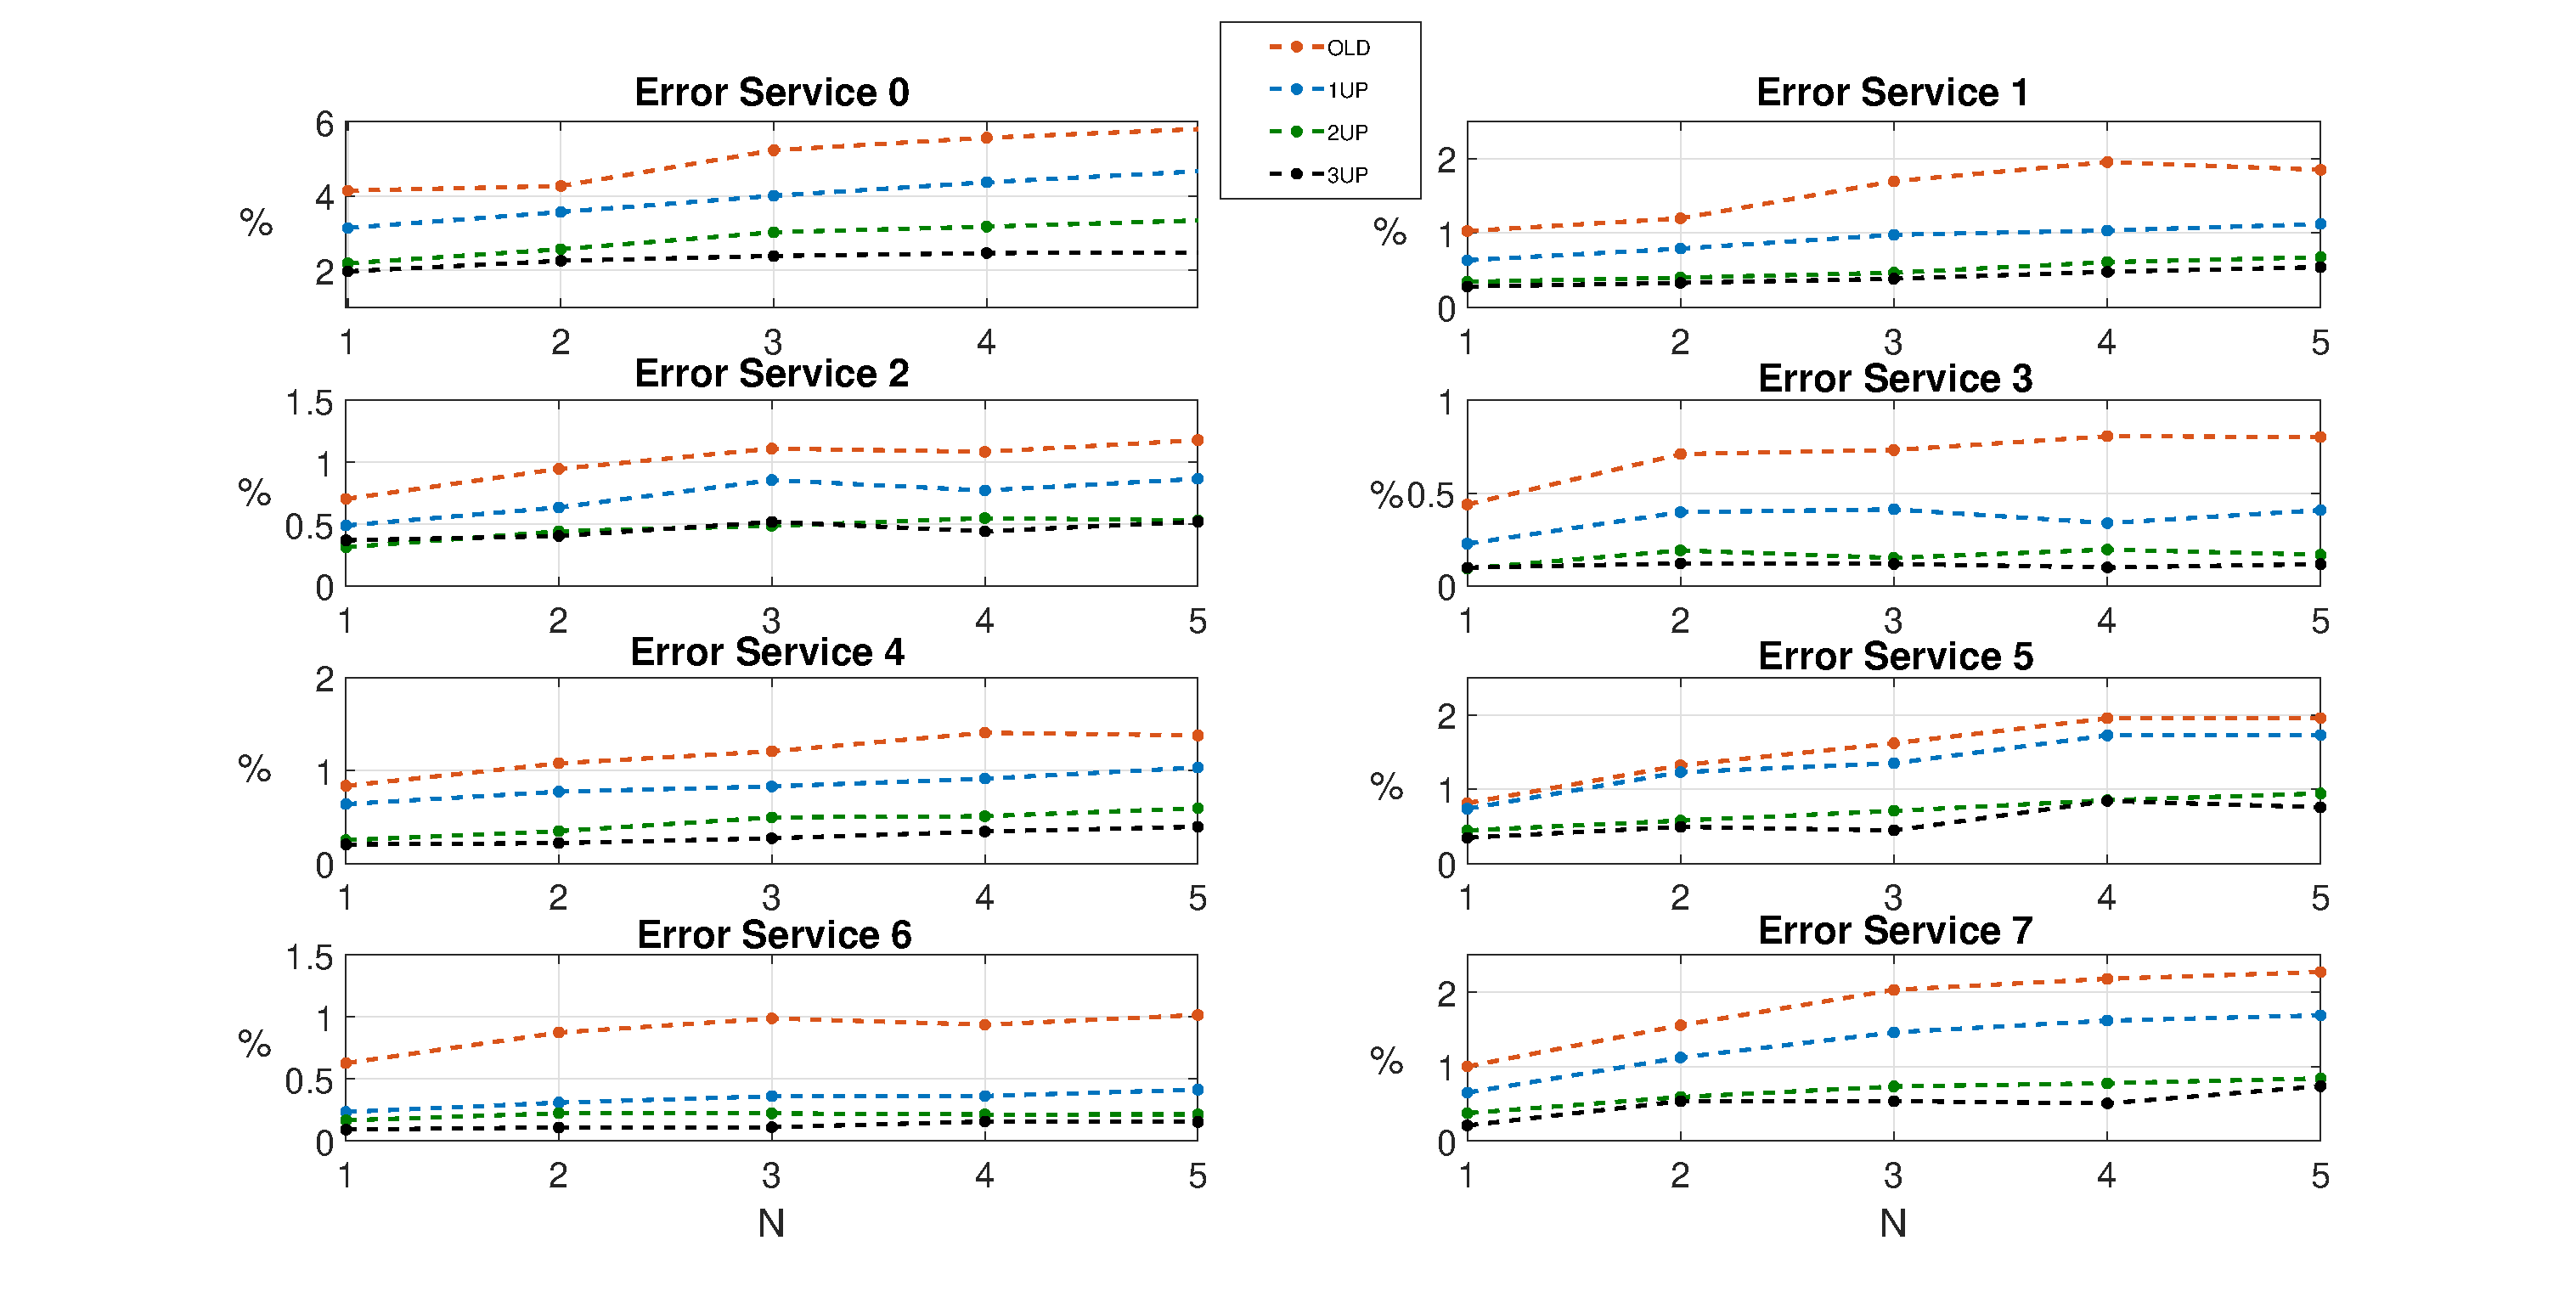
\includegraphics[trim={120 0 120 0}, width=1\linewidth]{figure/Error_Disturbance.eps}
	\caption{NRMSE of the disturbance predictive model over a time horizon of $N=5$.}
	\label{fig:{errorDist}}
\end{figure}
\begin{figure}[h!]
	\centering
	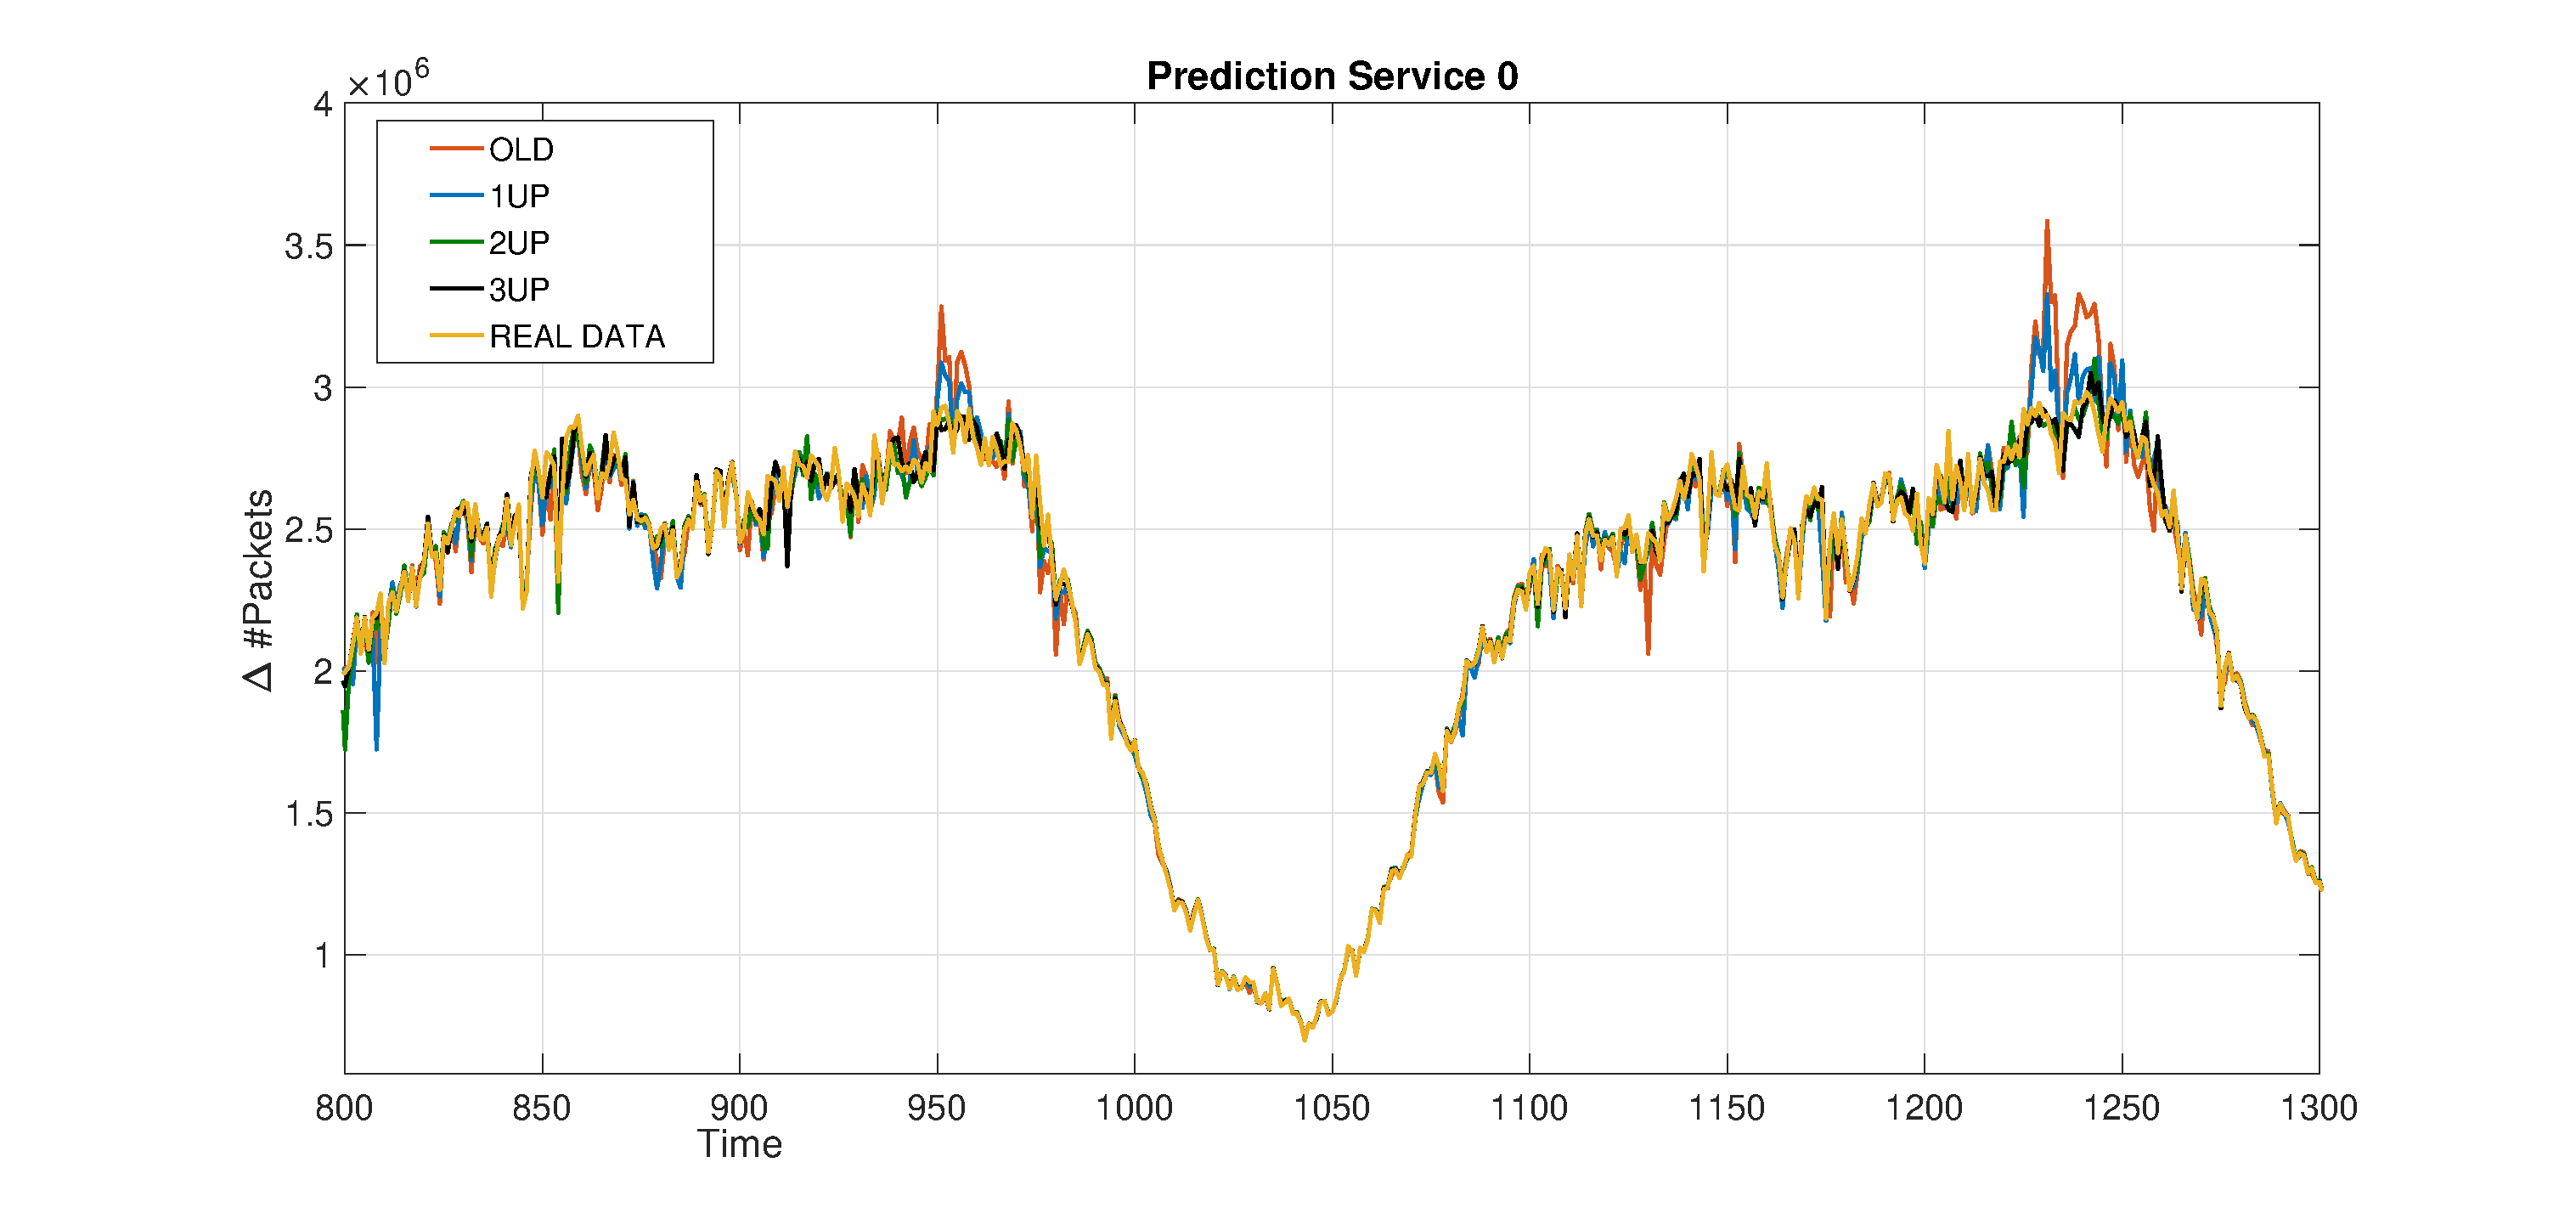
\includegraphics[trim={120 0 120 0}, width=1\linewidth]{figure/Error_Disturbance_Packets.eps}
	\caption{Comparison between the real traffic (YELLOW LINE) and the traffic prediction for the different models for Service 0.}
	\label{fig:{errorPack}}
\end{figure}

Figure \ref{fig:{errorDist}} shows the Normalised Root Mean Square Error (NRMSE) of the predictive model of the disturbance signals (one for each of the 8 DSCP indices) over a time horizon of $N=5$: the prediction error is worse for Service $0$ ($4-6\%$) since it includes the majority of the packets that transit through the switch. For other services the NRMSE is at most $2.2\%$ (Service 7) over all the predictive horizons. The improvement of the model accuracy when using larger (updated) data sets is evident, until a \textit{saturation} is reached and further data do not help to improve the model accuracy: the NRMSE significantly reduces and for Service 0 it is even halved. Figure \ref{fig:{errorPack}} plots, for Service $0$ and in a time window of $500$ samples (almost two days), the predictions of OLD, 1UP, 2UP and 3UP as well as the original data, and clearly highlights the better prediction of 2UP and 3UP with respect to OLD and 1UP.

%====================================================================================================

\subsection{Queues predictive model validation}

In this section we first compare the accuracy of our predictive models with Artificial Neural Networks. We recall that a neural network is a collection of algorithms that aim to identify underlying relations in a dataset: it consists of groups of connected neurons organized in layers, where the connections between neurons are modeled using weights. The signal produced with this linear composition is then fed into an activation function that is in general nonlinear. The reader is referred to \cite{NNstateOfART} and references therein for more details. A wide number of tools to build Neural Networks have been developed during recent years, e.g. \cite{tensorflow2015,chollet2015keras,openNN} just to mention a few: in this work we exploit the Deep Learning Toolbox of Matlab to compare predictive models based on NNs with the methodology proposed in this work, based on ARX combined RTs and RFs. We consider here just OLD as the learning dataset and chose a predictive horizon $N=5$.

To identify a RT (resp. RF) based predictive model of the queues we trained a Regression Tree (resp. a Random Forest) for each output and for each time horizon, with a total of $15$ trees (resp. $15$ forests each consisting of $30$ trees). The main parameters used for the identification algorithm (see Section \ref{secSwitchedModeling} and Problem \ref{pbLeastSquareProblem}) are summarized in Table \ref{tab:idPar}.  
\begin{table}[h!]
	\caption{Identification parameters}
	\centering
	\begin{tabular}{c c c c}
		\hline\hline
		Parameters & Value & Parameters & Values\\ 
		\hline
		N               & 5    & $f_{min}$   &-100 \\
		$\nu$        & 1     & $f_{max}$  &100  \\
		$\delta_x$ & 5     & $a_{min}$  &-100  \\
		$\delta_u$ & 5     & $a_{max}$ &100 \\
		$\delta_d$ & 5   & $b_{min}$  &0  \\
		Minleaf      & 13   & $b_{max}$ &10000  \\
		$|\Fij|$      & 30  &                   &\\
		\hline
	\end{tabular}
	\label{tab:idPar}
\end{table}
In particular, the regressive terms ($\delta_d$, $\delta_x$, $\delta_u$) and the minimum number of samples for each tree of each forest (MinLeaf) have been chosen, with a trial and error approach, considering that very small regressive horizons and very large values for MinLeaf may lead to inaccurate prediction (as they do not provide sufficient information on the past) but very large regressive horizons and very small values for MinLeaf also lead to inaccurate prediction (as they interpolate very old data that might negatively affect the results and produce overfitting).

Regarding specific parameters used for running NN, and for the sake of a fair comparison, we tuned them to obtain the best performance: in particular we considered shallow networks of 2 layers since depper networks did not improve the accuracy and, instead, have the negative effect of increasing the sensitivity of the accuracy with respect to the initial conditions of the weights. Among the many algorithms for optimizing the weights of the neurons we exploited the \textit{Scaled conjugate gradient back-propagation} described in \cite{Moller1990}, which provided the best accuracy with respect to our dataset. Regarding the activation functions, we used both the classical sigmoid function (\textit{LogSig}) and the Hyperbolic tangent sigmoid transfer function (\textit{TanSig}).
\begin{figure}[h!]
	\centering
	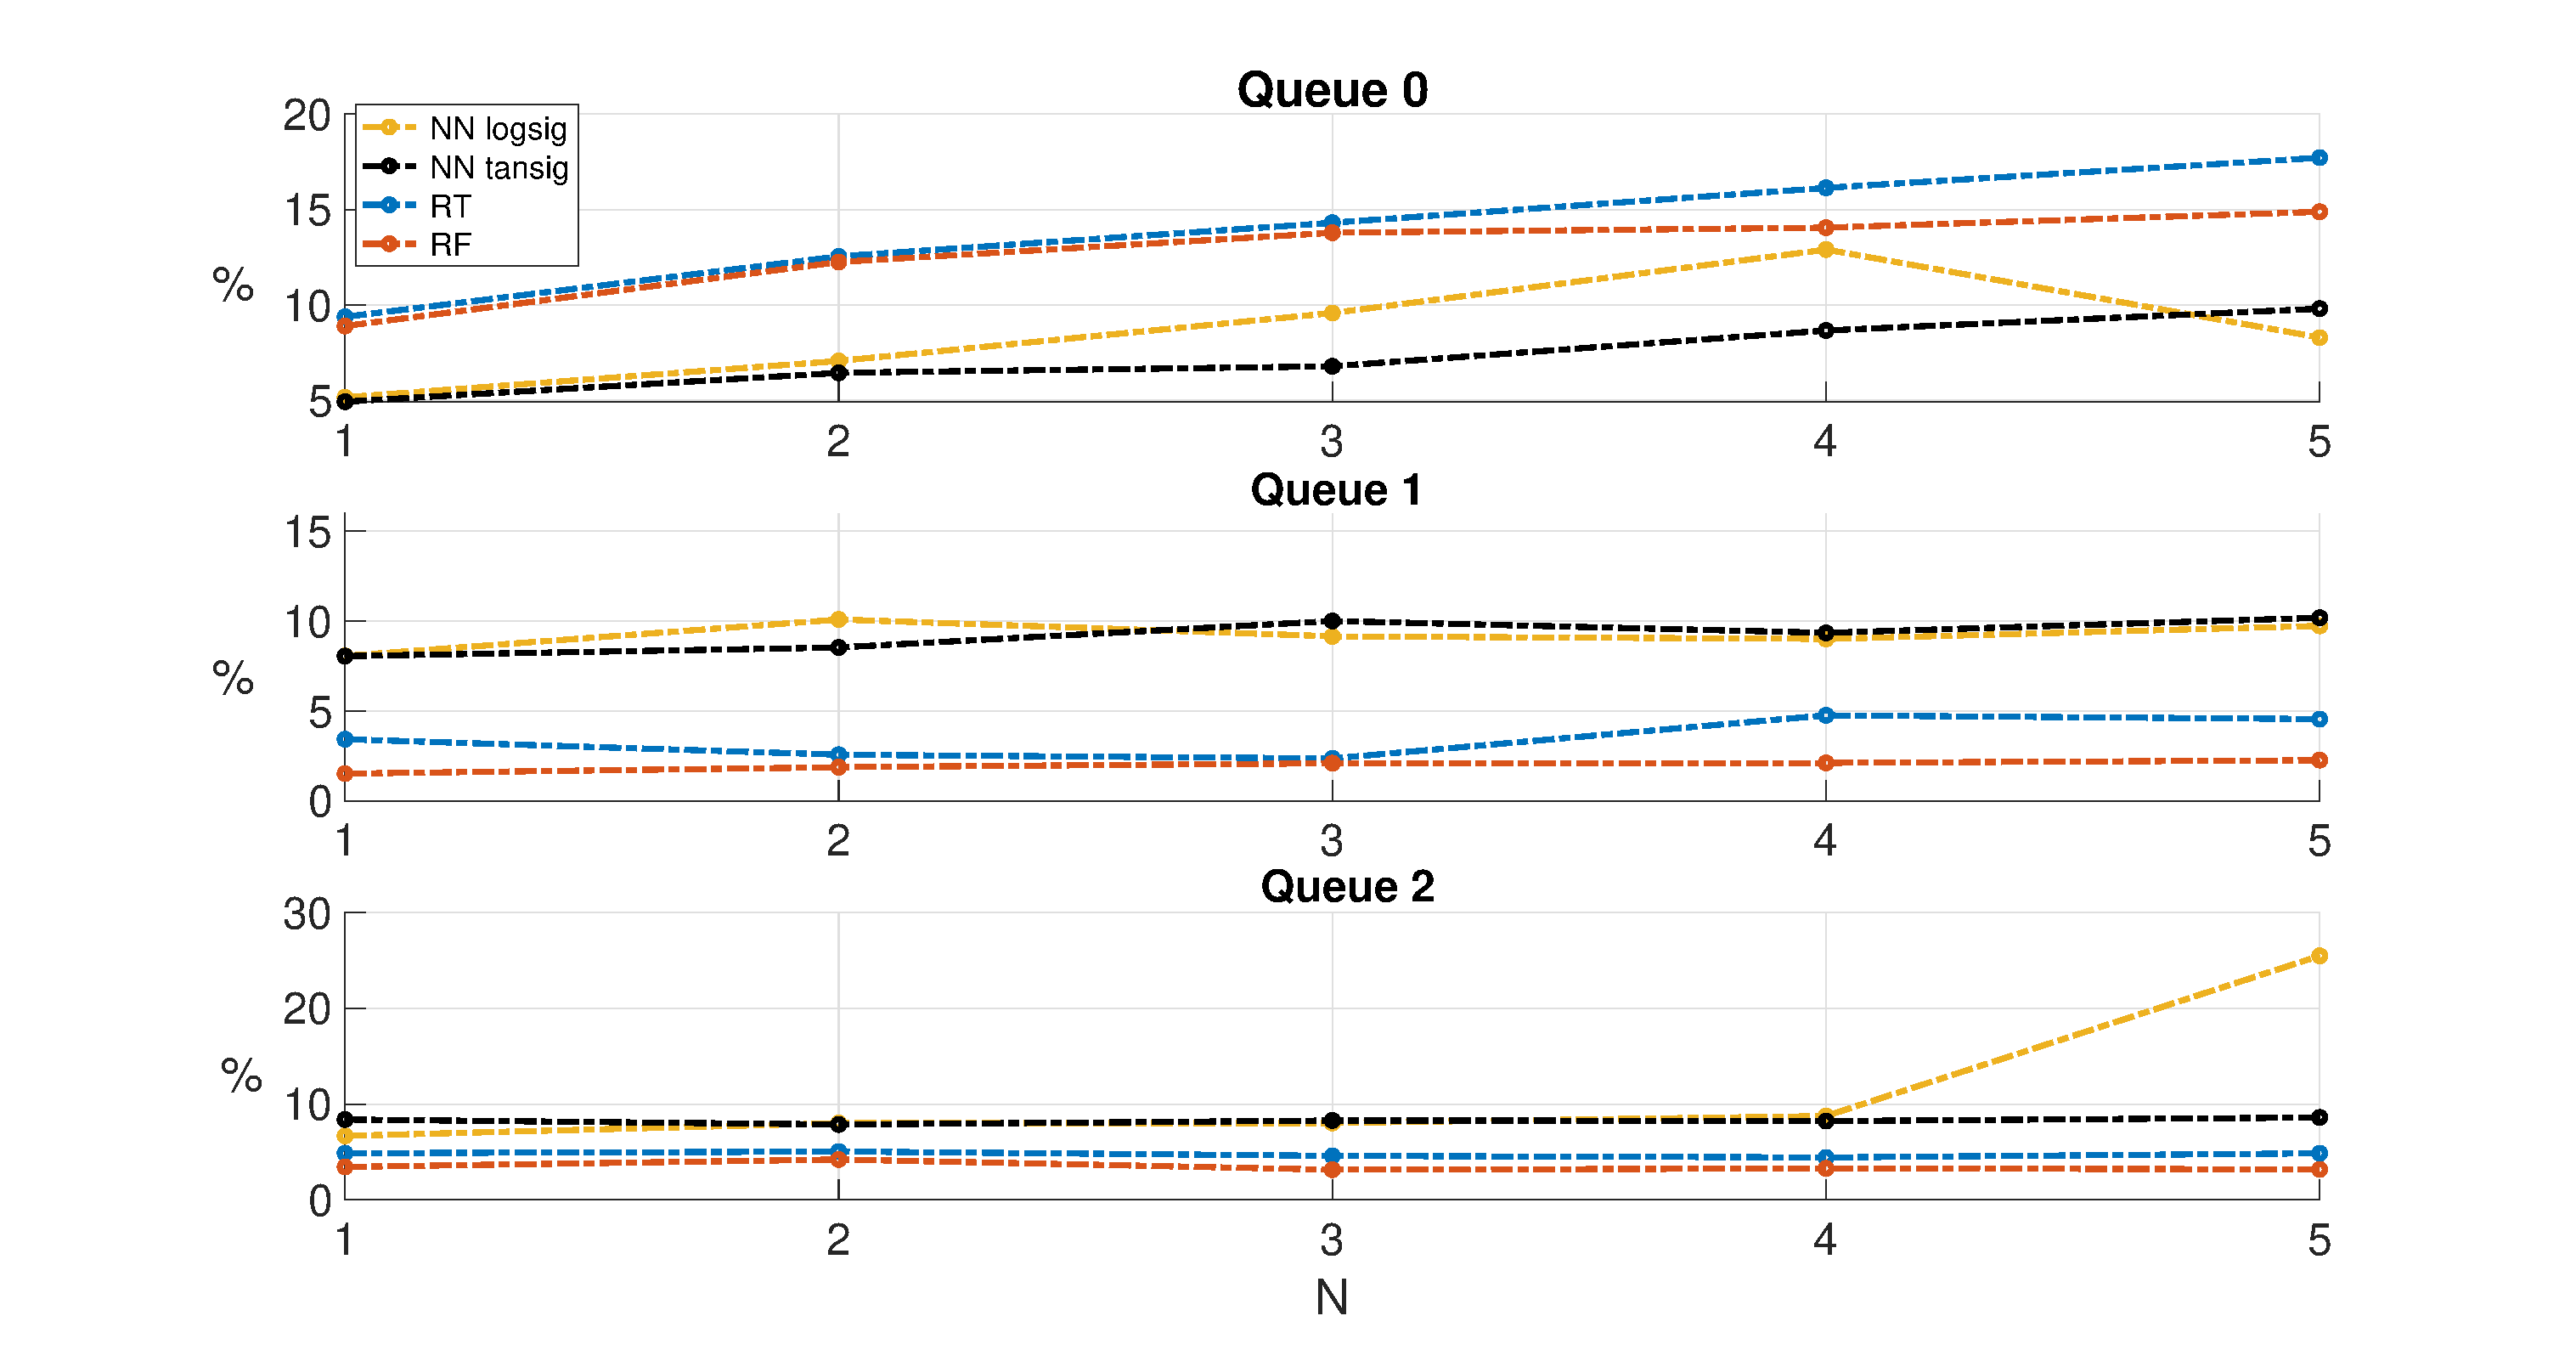
\includegraphics[trim={120 0 120 0},width=0.9\linewidth]{figure/NRMSENNvsRTvsRF.eps}
	\vspace{-0.2cm}
	\caption{NRMSE, up to $N=5$ and for each priority class, for RT (blue), RF (red), NN with sigmoids as activation function (yellow) and NN with hyperbolic tangent as activation function (black).}
	\label{fig:{NRMSE}}
\end{figure}

As a metric of the prediction accuracy we compared in Figure \ref{fig:{NRMSE}} the Normalized Root Mean Square Errors (NRMSE) of the different identification approaches for each priority class and over a horizon up to $N=5$. Regarding queue $0$ (Default) NNs perform better than RT and RF, but in queues $1$ (Premium) and $2$ (Gold), characterised by higher priority, RF provides the best performance. Queue $0$ is characterised by a larger NRMSE with all identification techniques: this is due to the fact that, having the lowest priority, it suffers more packet losses and this can negatively affect the prediction accuracy. Our validation emphasizes that RTs, even thought very simple and fast to compute, are often affected by overfitting and variance issues, i.e. small variations of the training data result in large variations of the tree structure and, consequently, of the predictions. Regarding NNs, they provide a less accurate model in 2 cases over 3. Indeed, by analyzing the dataset distribution (see Figure \ref{fig:{datadistribution}}), we noticed a peculiar regular grid pattern that can be very well approximated by hyper-rectangles: since RTs and RFs base their prediction on hyper-rectangular dataset partitions, the better performance with respect to NNs is reasonable.
\begin{figure}[h!]
	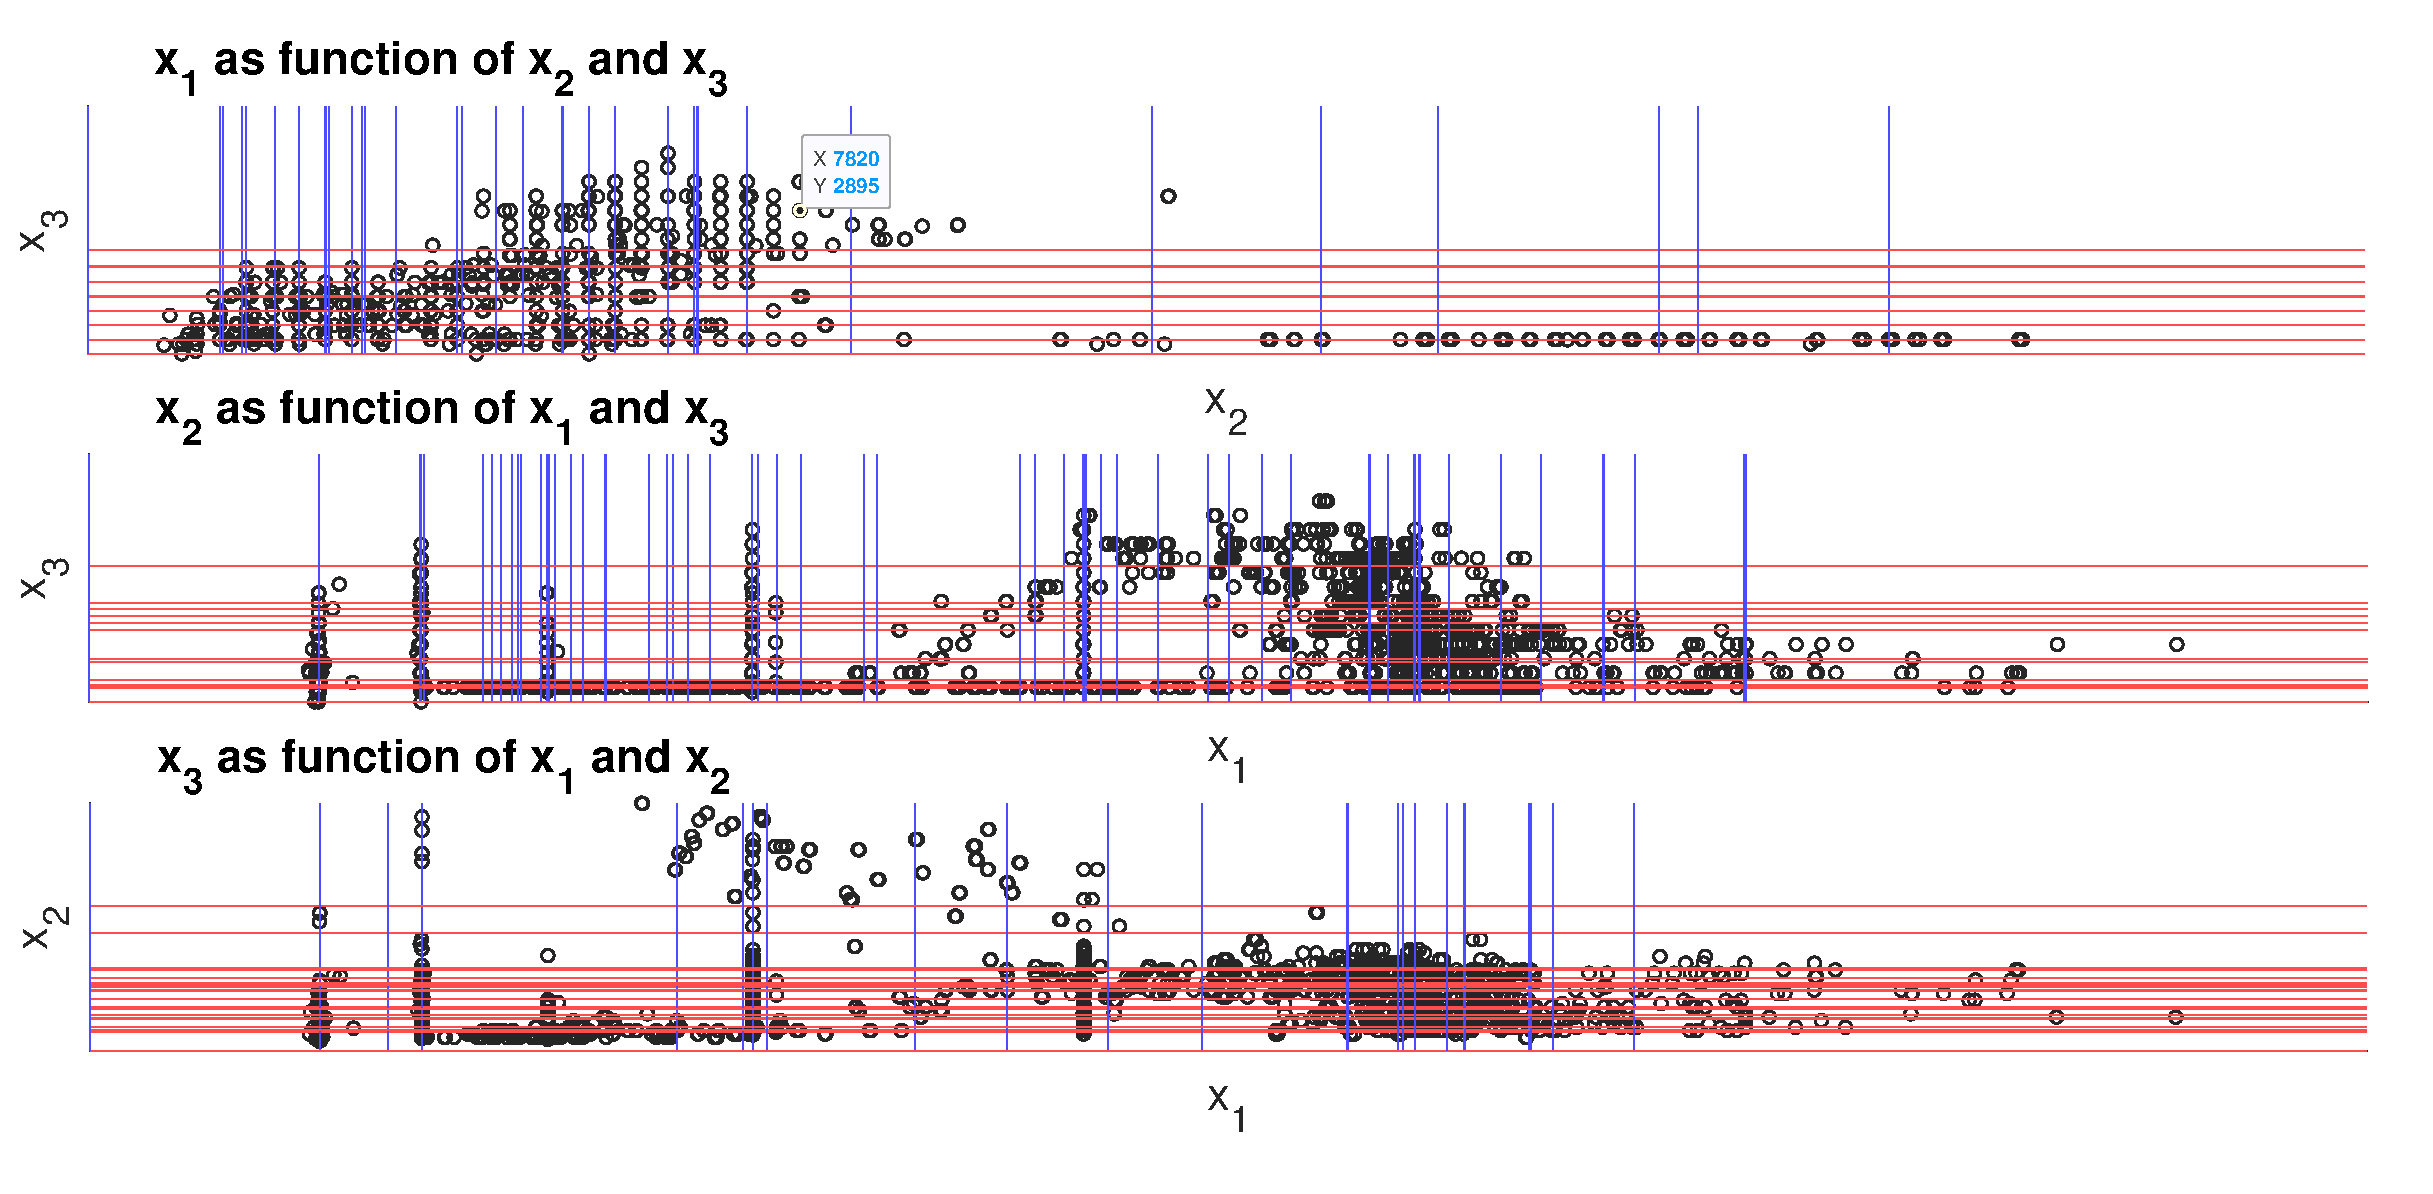
\includegraphics[width=\linewidth]{figure/datadistribution.eps}
	\caption{Grid pattern emerged from dataset distribution.}
	\label{fig:{datadistribution}}
\end{figure}
For queue 0, even thought NNs perform better, we need to remark that their predictive model is based on nonlinear functions: this makes the derived model impractical for real-time control as the corresponding MPC formulation turns into a nonlinear optimization problem, for which there is no approach that can guarantee neither a global optimal solution nor a reasonable computation time. In addition to this, even obtaining a closed mathematical form of the predictive function of a Neural Network starting from neurons and weitghts is not always an easy task, because of the highly nonlinear interconnections between the different layers. For all these reasons we decided to only use from now on RF-based models, which provide the best choice both from the accuracy and the computational complexity points of view. In the following we illustrate the effect of iterative dataset updates in the prediction accuracy, both with and without knowledge of the future disturbances.
\begin{figure}[th!]
	\centering
	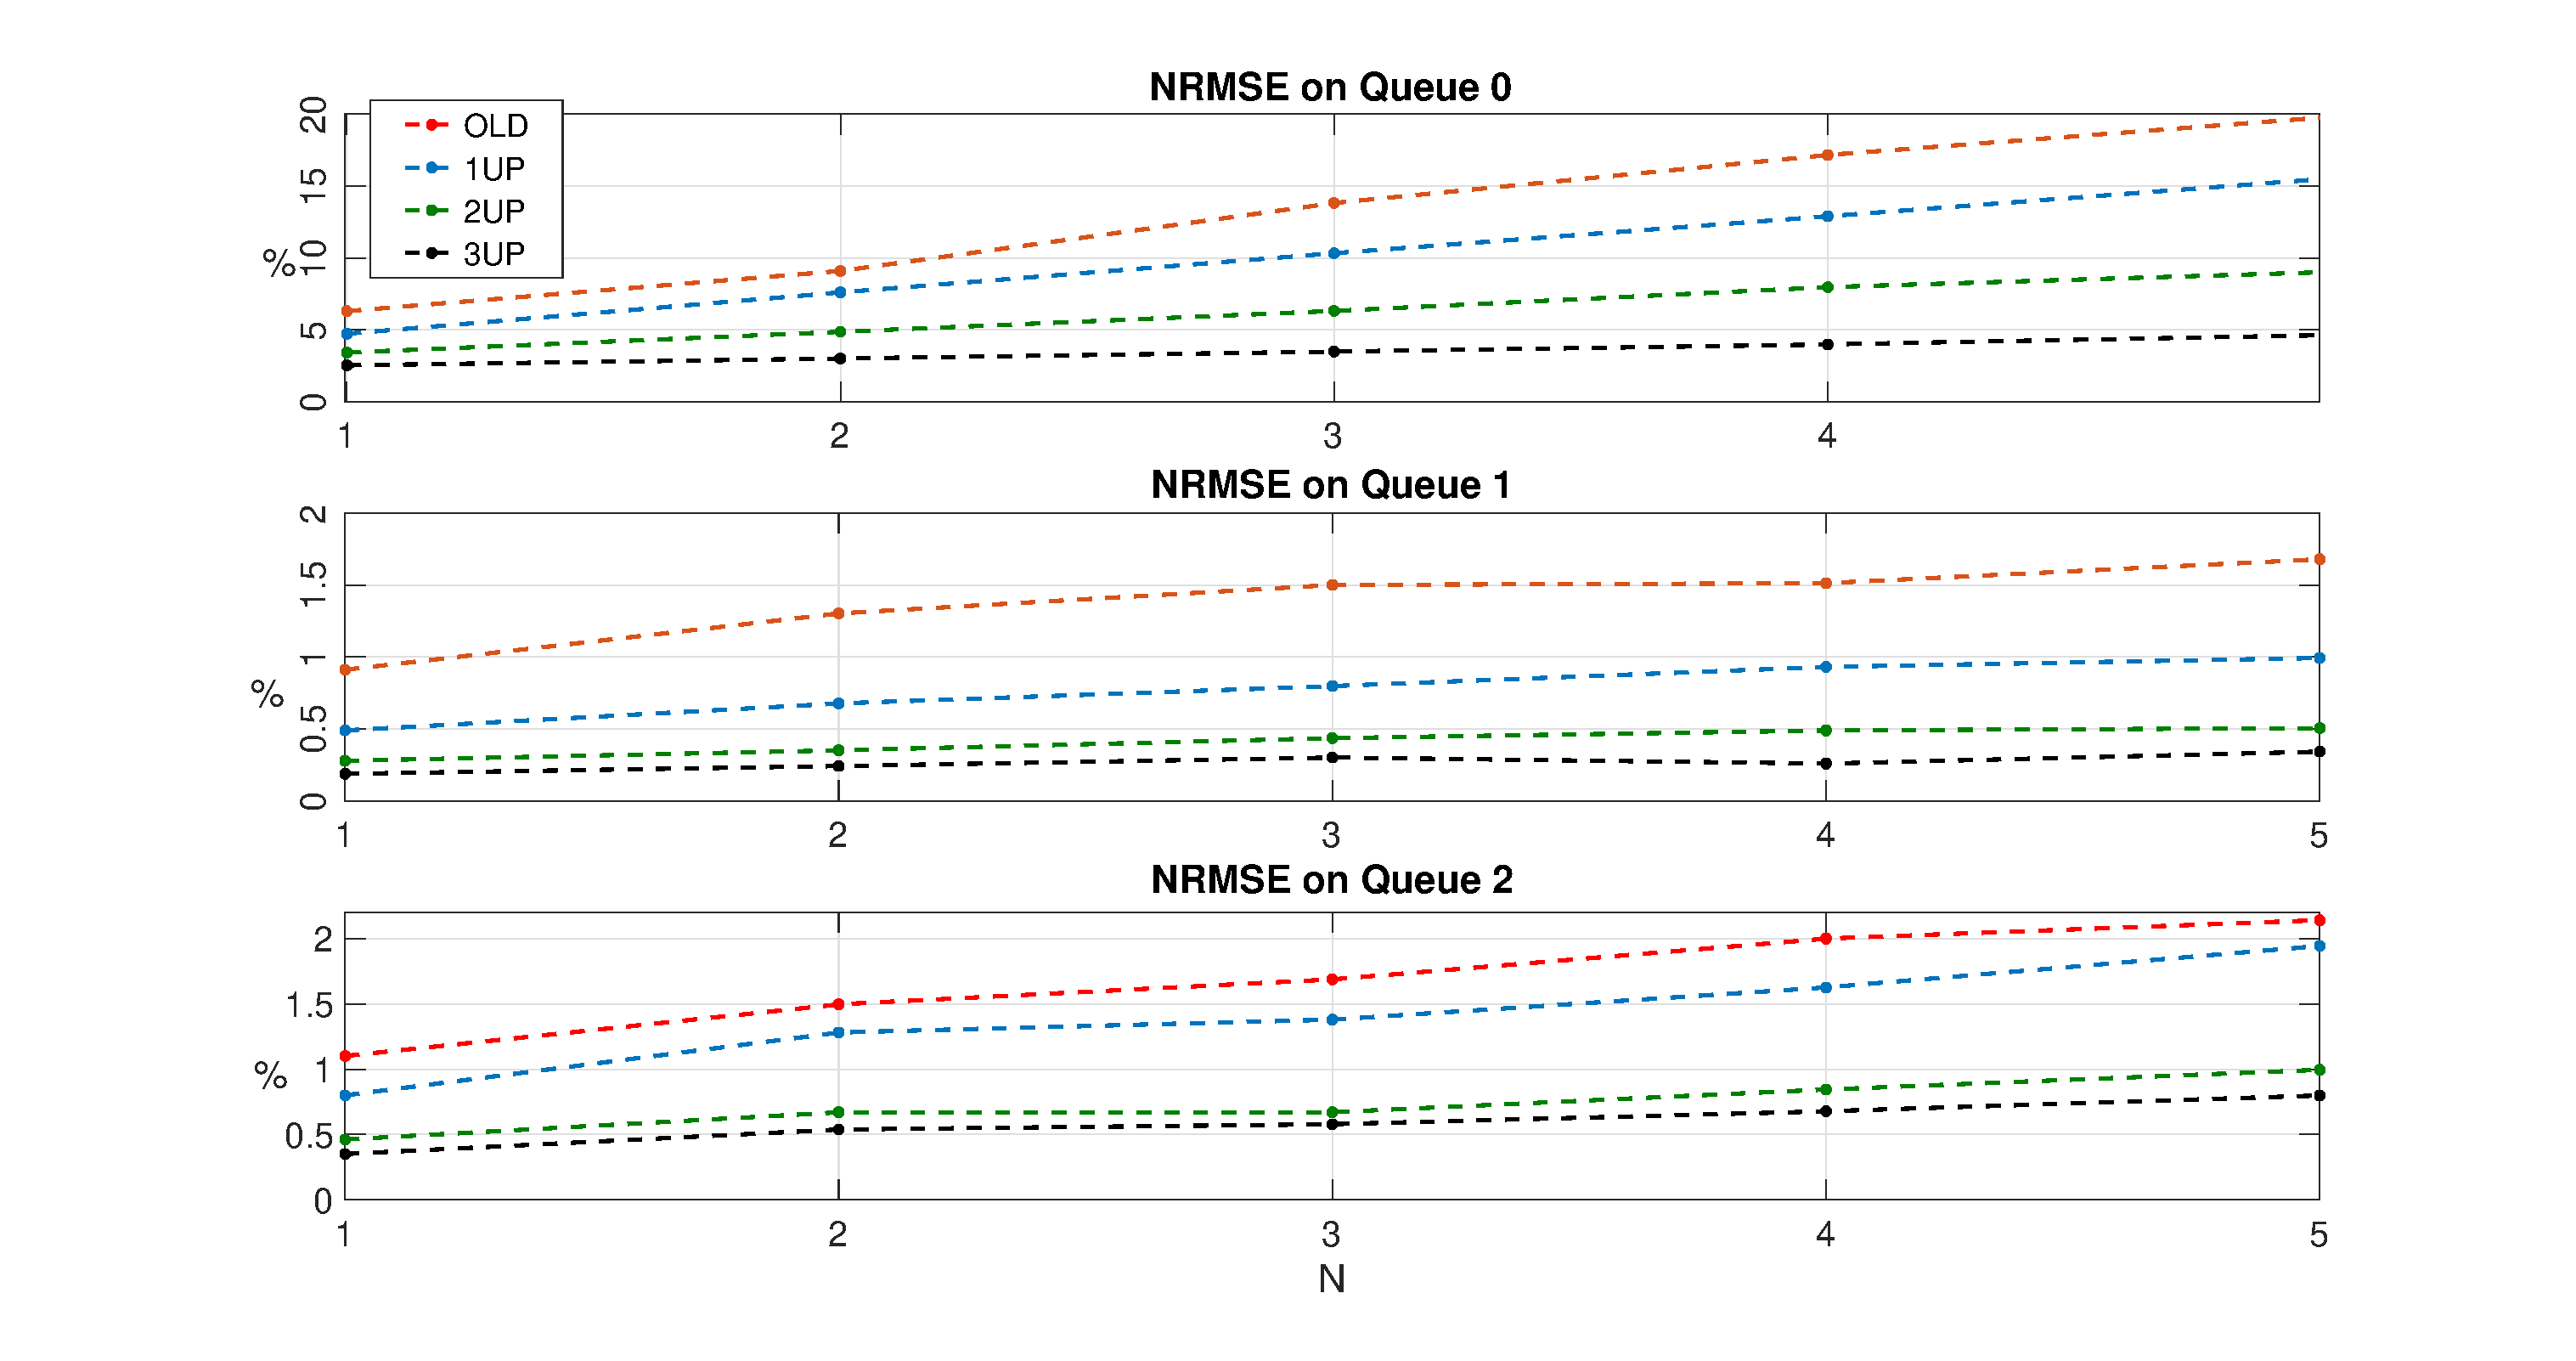
\includegraphics[trim={120 0 120 0}, width=0.9\linewidth]{figure/Error_State.eps}
	\caption{NRMSE of the queues output predictive model over a time horizon of $N=5$, without knowledge of the future disturbances}
	\label{fig:{stateNRMSE}}
\end{figure}
\begin{figure}[th!]
	\centering
	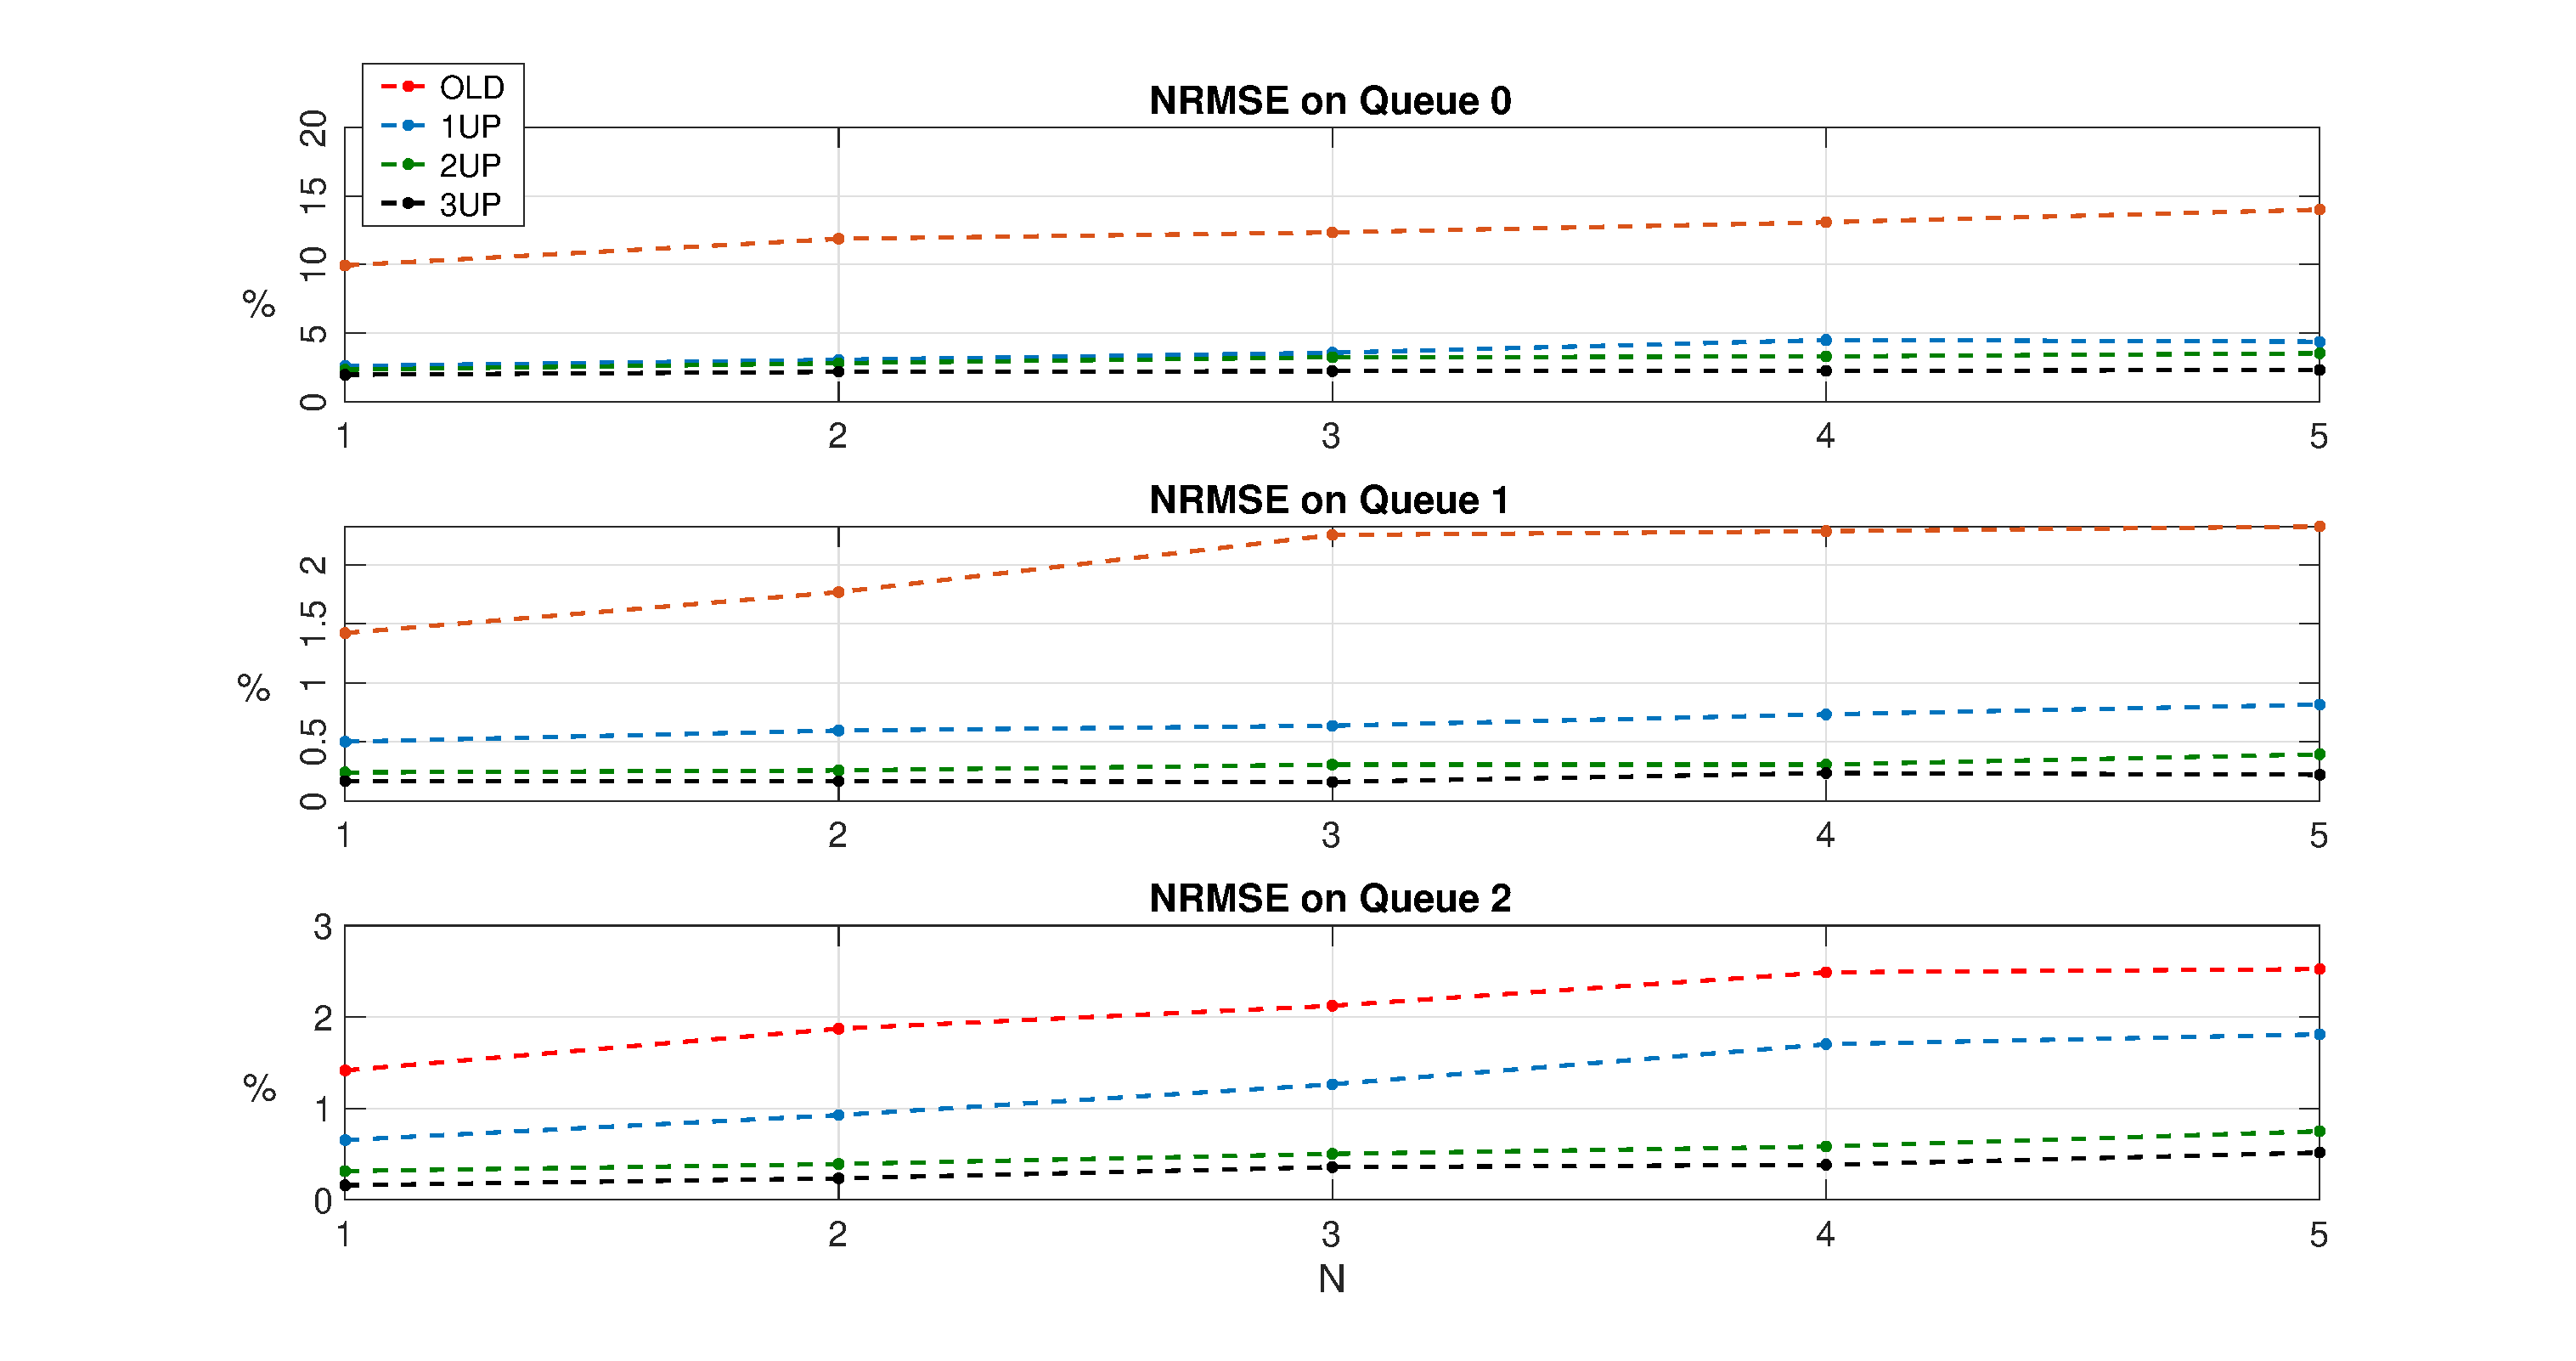
\includegraphics[trim={120 0 120 0}, width=0.9\linewidth]{figure/Error_State_ddM4.eps}
	\caption{NRMSE of the queues output predictive model over a time horizon of $N=5$, with knowledge of the 4-steps future disturbances}
	\label{fig:{stateNRMSEddM4}}
\end{figure}

Figure \ref{fig:{stateNRMSE}} and Figure \ref{fig:{stateNRMSEddM4}} plot the NRMSEs respectively without and with knowledge of the future disturbances. The assumption of future disturbance forecast, as expected, provides much better prediction accuracy. The positive effect of updated data sets is also clear, providing accuracy improvements up to $50 \%$: as will be also discussed in the next section, the most relevant prediction accuracy improvement takes place moving from OLD to 1UP or from 1UP to 2UP, while the 3UP model does not improve much.

\begin{remark}
We wish to highlight that in our simulations we generated data without major modifications of the traffic daily pattern: for this reason enriching the data set converges to a saturation of the model accuracy, as discussed above. Nevertheless, the capability of our methodology to iteratively learn from new data is fundamental as, in real life, changes in the traffic patterns do occur, and model updates are necessary to maintain the model accuracy and the control performance. 
\end{remark}

%====================================================================================================

\subsection{Control performance}\label{sec:control_performance}

In this section we setup a control loop where the (Mininet) network emulator and the (Ryu) controller run in two different computers, and synchronize/exchange data using a shared file. Namely, our SW controller module is, in principle, ready to be directly used on a real SDN-based network, with just some minor modifications in the data exchange with the switch devices. The controller implements MPC using the predictive models validated in the previous sections: at each time step, it solves Problem \ref{pbMPC} and optimally updates the bandwidth of the different queues. The cost matrices $Q$ and $R$ of Problem \ref{pbMPC} respectively weight the output $y(k)$ of the system (i.e. the packet transmission rate for each queue) and the control input $u(k)$ (i.e. the bandwidth assigned to each queue). Since $R$ is required to be positive definite but it makes no sense assigning a penalty to the choice of $u(k)$, we define $R=10^{-5} \cdot \mathbb I$, where the identity matrix $\mathbb I$ multiplies a very small value. Matrix $Q = diag(1,10^4,10)$ has been assigned as a diagonal matrix, where the choice of the different diagonal components is related to the priority level of each queue. The remaining constraints of Problem \ref{pbMPC} are reported in Table \ref{tab:contPar}.
%The parameters used in the constraints described in Problem \ref{pbMPC} are reported in Table \ref{tab:contPar} and the weights matrices considered in the optimisation cost are: $Q=diag([1,1000,10])$ and $R=10^{-5} \mathbb{I}_3$.
\begin{table}[h!]
	\caption{Constraints in Problem \ref{pbMPC}}
	\centering
	\begin{tabular}{l c l c}
		\hline\hline
		Parameters                                & Value               & Parameters                 & Values       \\ 
		\hline
		$\Delta u_1^\mathrm{min}$     & 1                   & $\Delta u_1^\mathrm{max}$  & 30           \\
		$\Delta u_2^\mathrm{min}$     & 20                  & $\Delta u_2^\mathrm{max}$  & 30           \\
		$\Delta u_3^\mathrm{min}$     & 20                  & $\Delta u_3^\mathrm{max}$  & 20           \\
		$u_1^\mathrm{min} $             & 10                  & $u_1^\mathrm{max} $        & 45           \\
		$u_2^\mathrm{min} $            & 55                  & $u_2^\mathrm{max} $        & 80           \\
		$u_3^\mathrm{min} $            & 80                  & $u_3^\mathrm{max} $        & 100          \\
		
		\hline
	\end{tabular}
	\label{tab:contPar}
\end{table}
In what follows we validate the control performance both without and with knowledge of the future disturbances. The value of $x_\mathrm{ref}$ in the optimization problem represents the reference value we chose for tracking system output: indeed, as we wish to minimize packet losses, we minimize the difference between the packets received by the hosts $d(k)$ and those transmitted by the queues $y(k)$ over the horizon $N$. In case we have no knowledge of future disturbances, we consider $x_\mathrm{ref}$ equal to the current disturbance  measurement $d(k)$ and constant over all the predictive horizon; if instead we have knowledge of future disturbances, we consider $x_\mathrm{ref}$ equal to such future disturbances. In this section we decided to only compare models OLD, 1UP and 2UP, since model 3UP does not provide any substantial improvement. 

 \begin{figure}[h!]
	\centering
	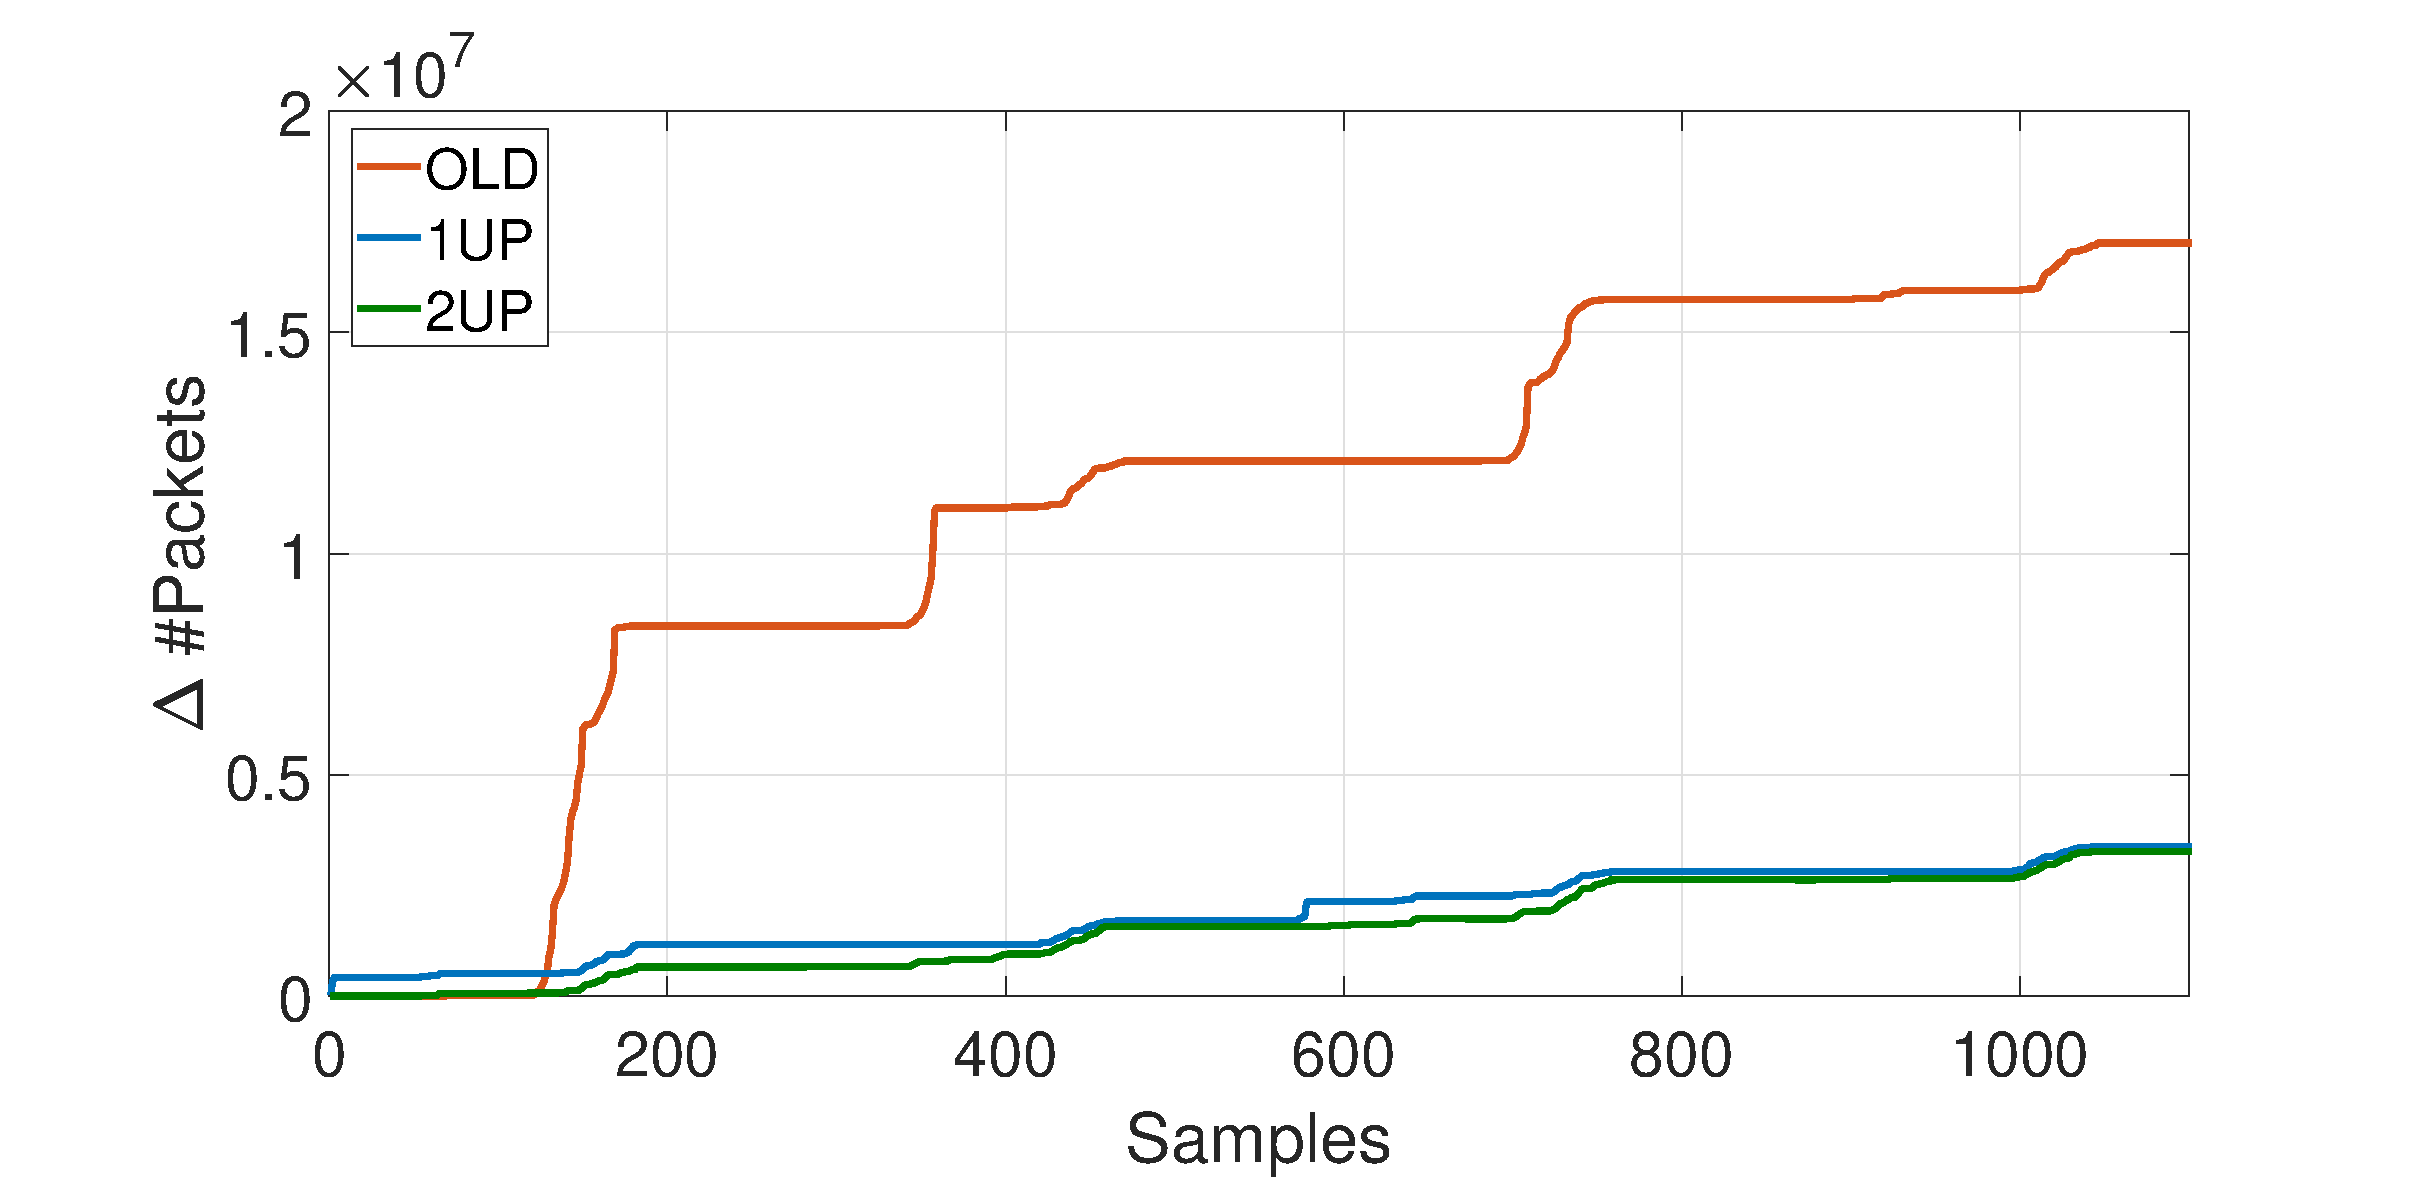
\includegraphics[trim={120 0 120 0}, width=0.9\linewidth]{figure/cumPL1.eps}
	\caption{Cumulative Packet Losses without knowledge of the future disturbance.}
	\label{fig:{MPC1}}
\end{figure}
\begin{figure}[h!]
	\centering
	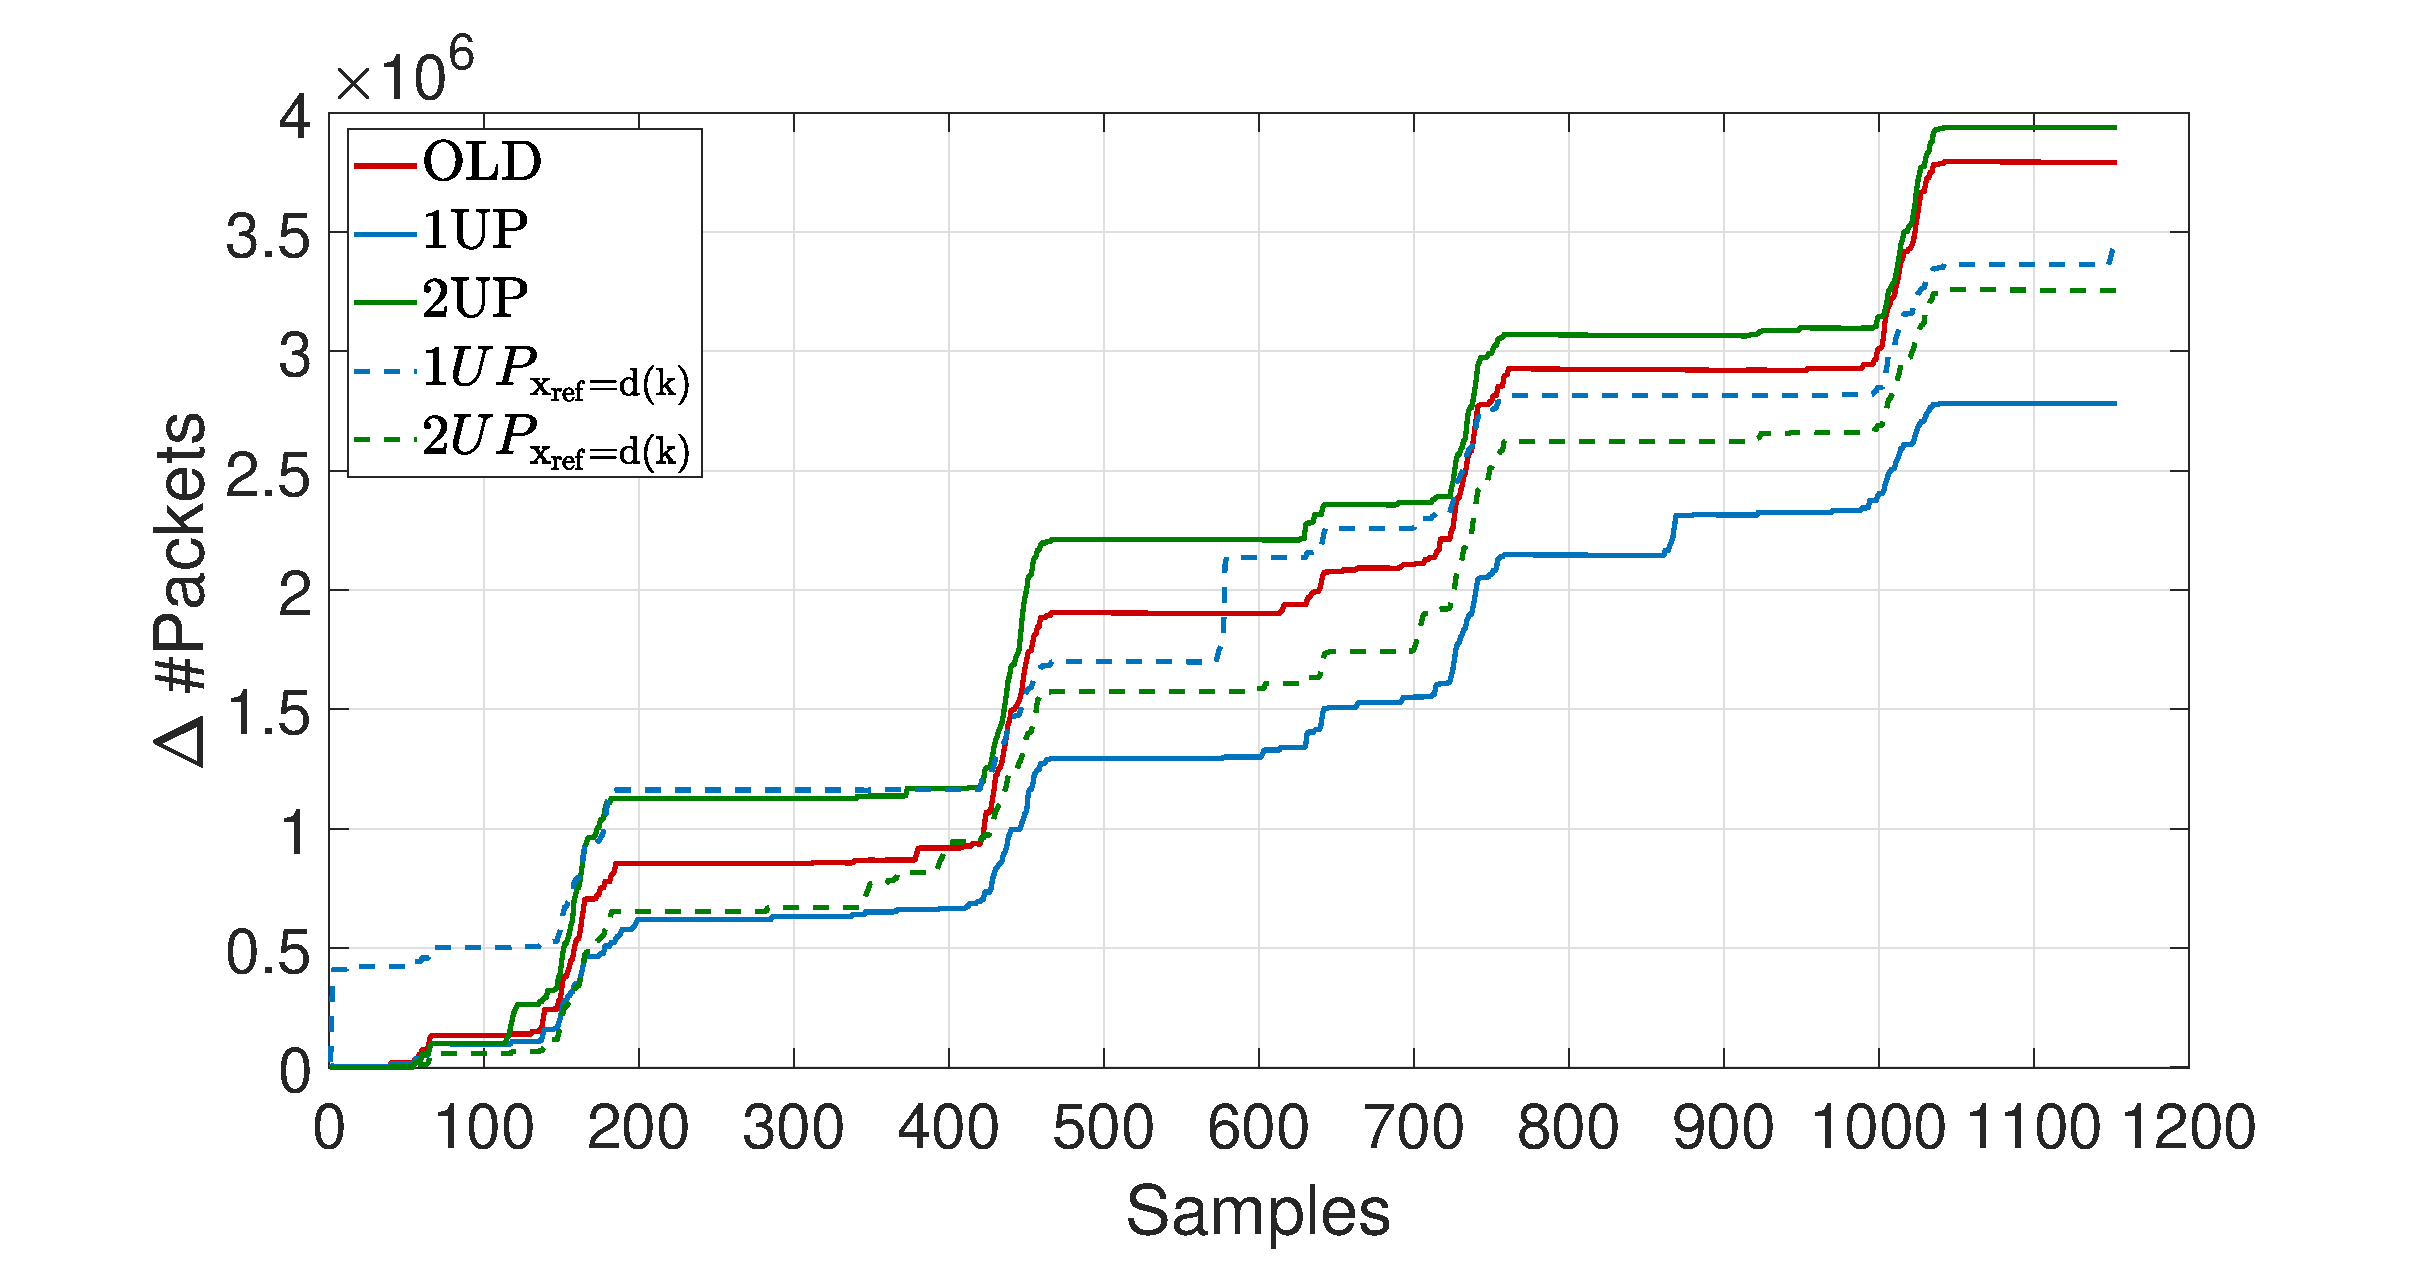
\includegraphics[trim={120 0 120 0},width=0.9\linewidth]{figure/cumPL_Total.eps}
	\caption{Comparison between Cumulative Packet Losses with (solid lines)  and without (dashed lines) knowledge of the future disturbance.}
	\label{fig:{MPC2}}
\end{figure}
 Figures \ref{fig:{MPC1}} and \ref{fig:{MPC2}} plot the cumulative packet losses respectively without and with knowledge of the future disturbances. The packet loss rate when the control is performed exploiting the OLD model and without disturbance forecast is around $123\%$ larger than all other cases (and, of course, incomparably smaller than the static control case \cite{Notiziario}). It is also clear from the plots that 1UP and 2UP without disturbance forecast and OLD, 1UP and 2UP with disturbance forecast provide very similar performance. Our interpretation is that OLD models without disturbance forecast have not enough information to provide good accuracy, but they can be easily improved either with a data set update (which however requires $10$ days for 1UP and $20$ days for 2UP of additional data) or using a predictive disturbance model.

\begin{figure}[h!]
\centering
\subfigure[a][]{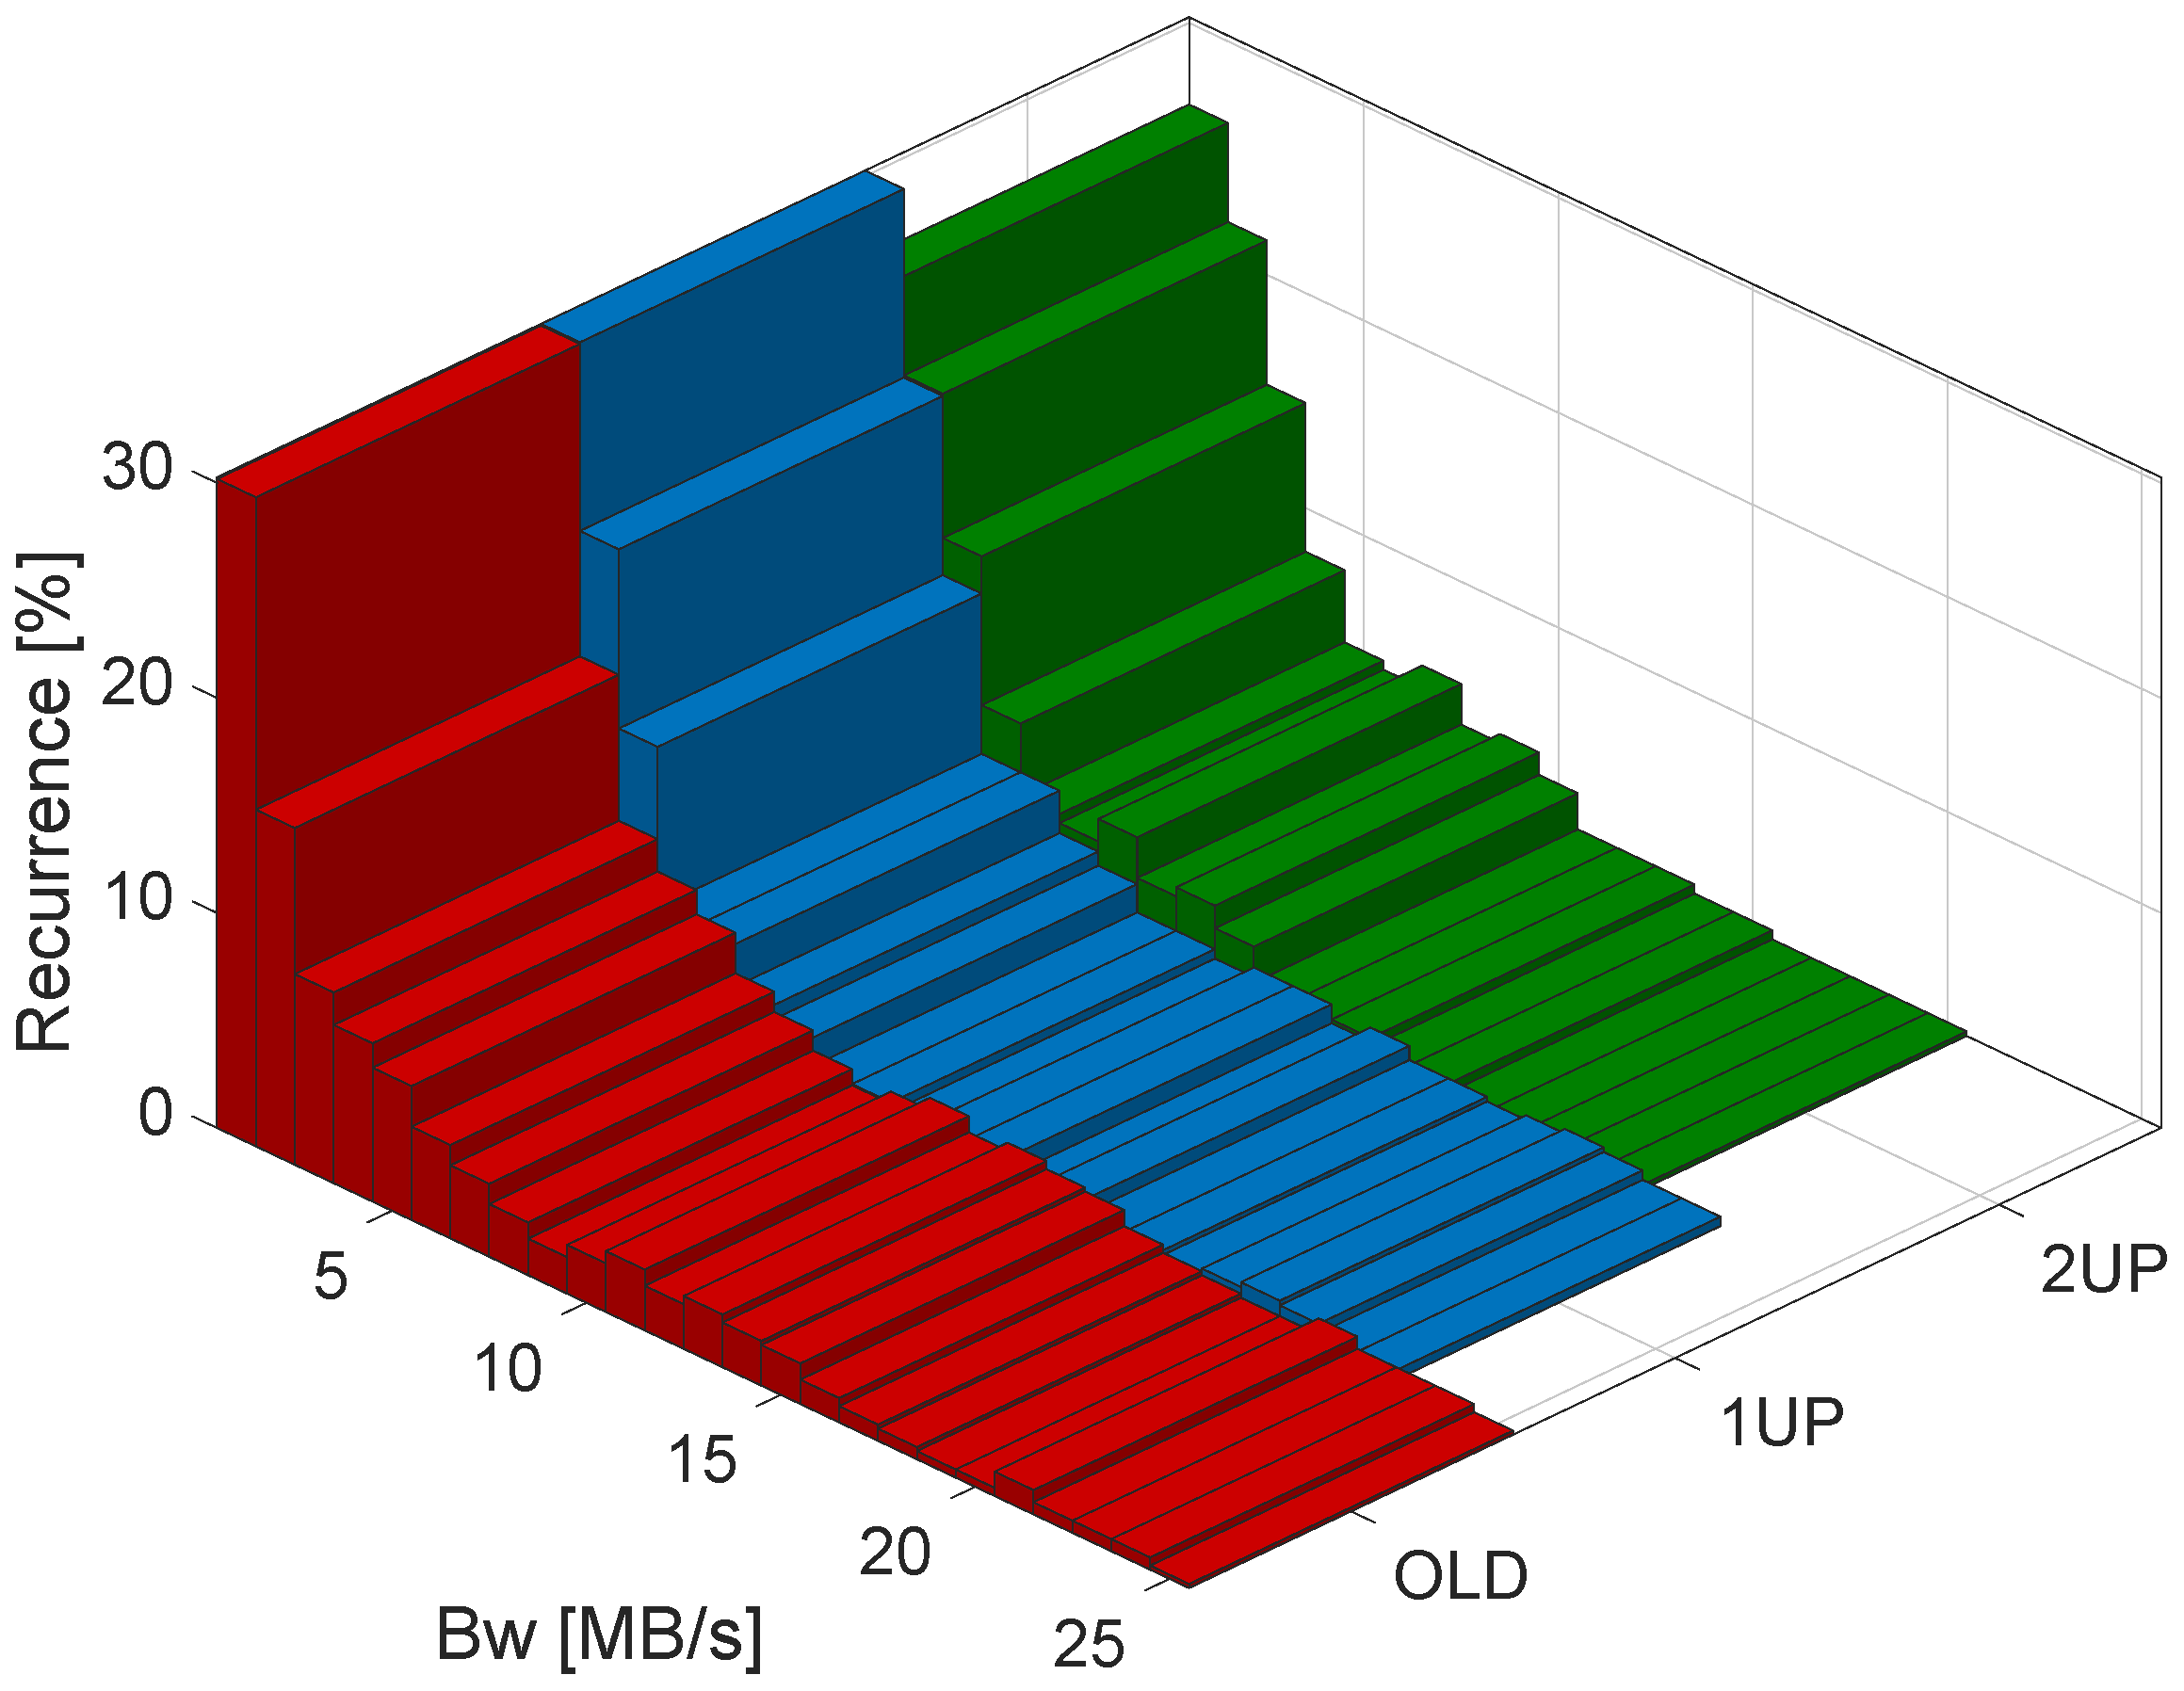
\includegraphics[width=0.7\linewidth]{figure/BW_NoPred.eps}}
\subfigure[b][]{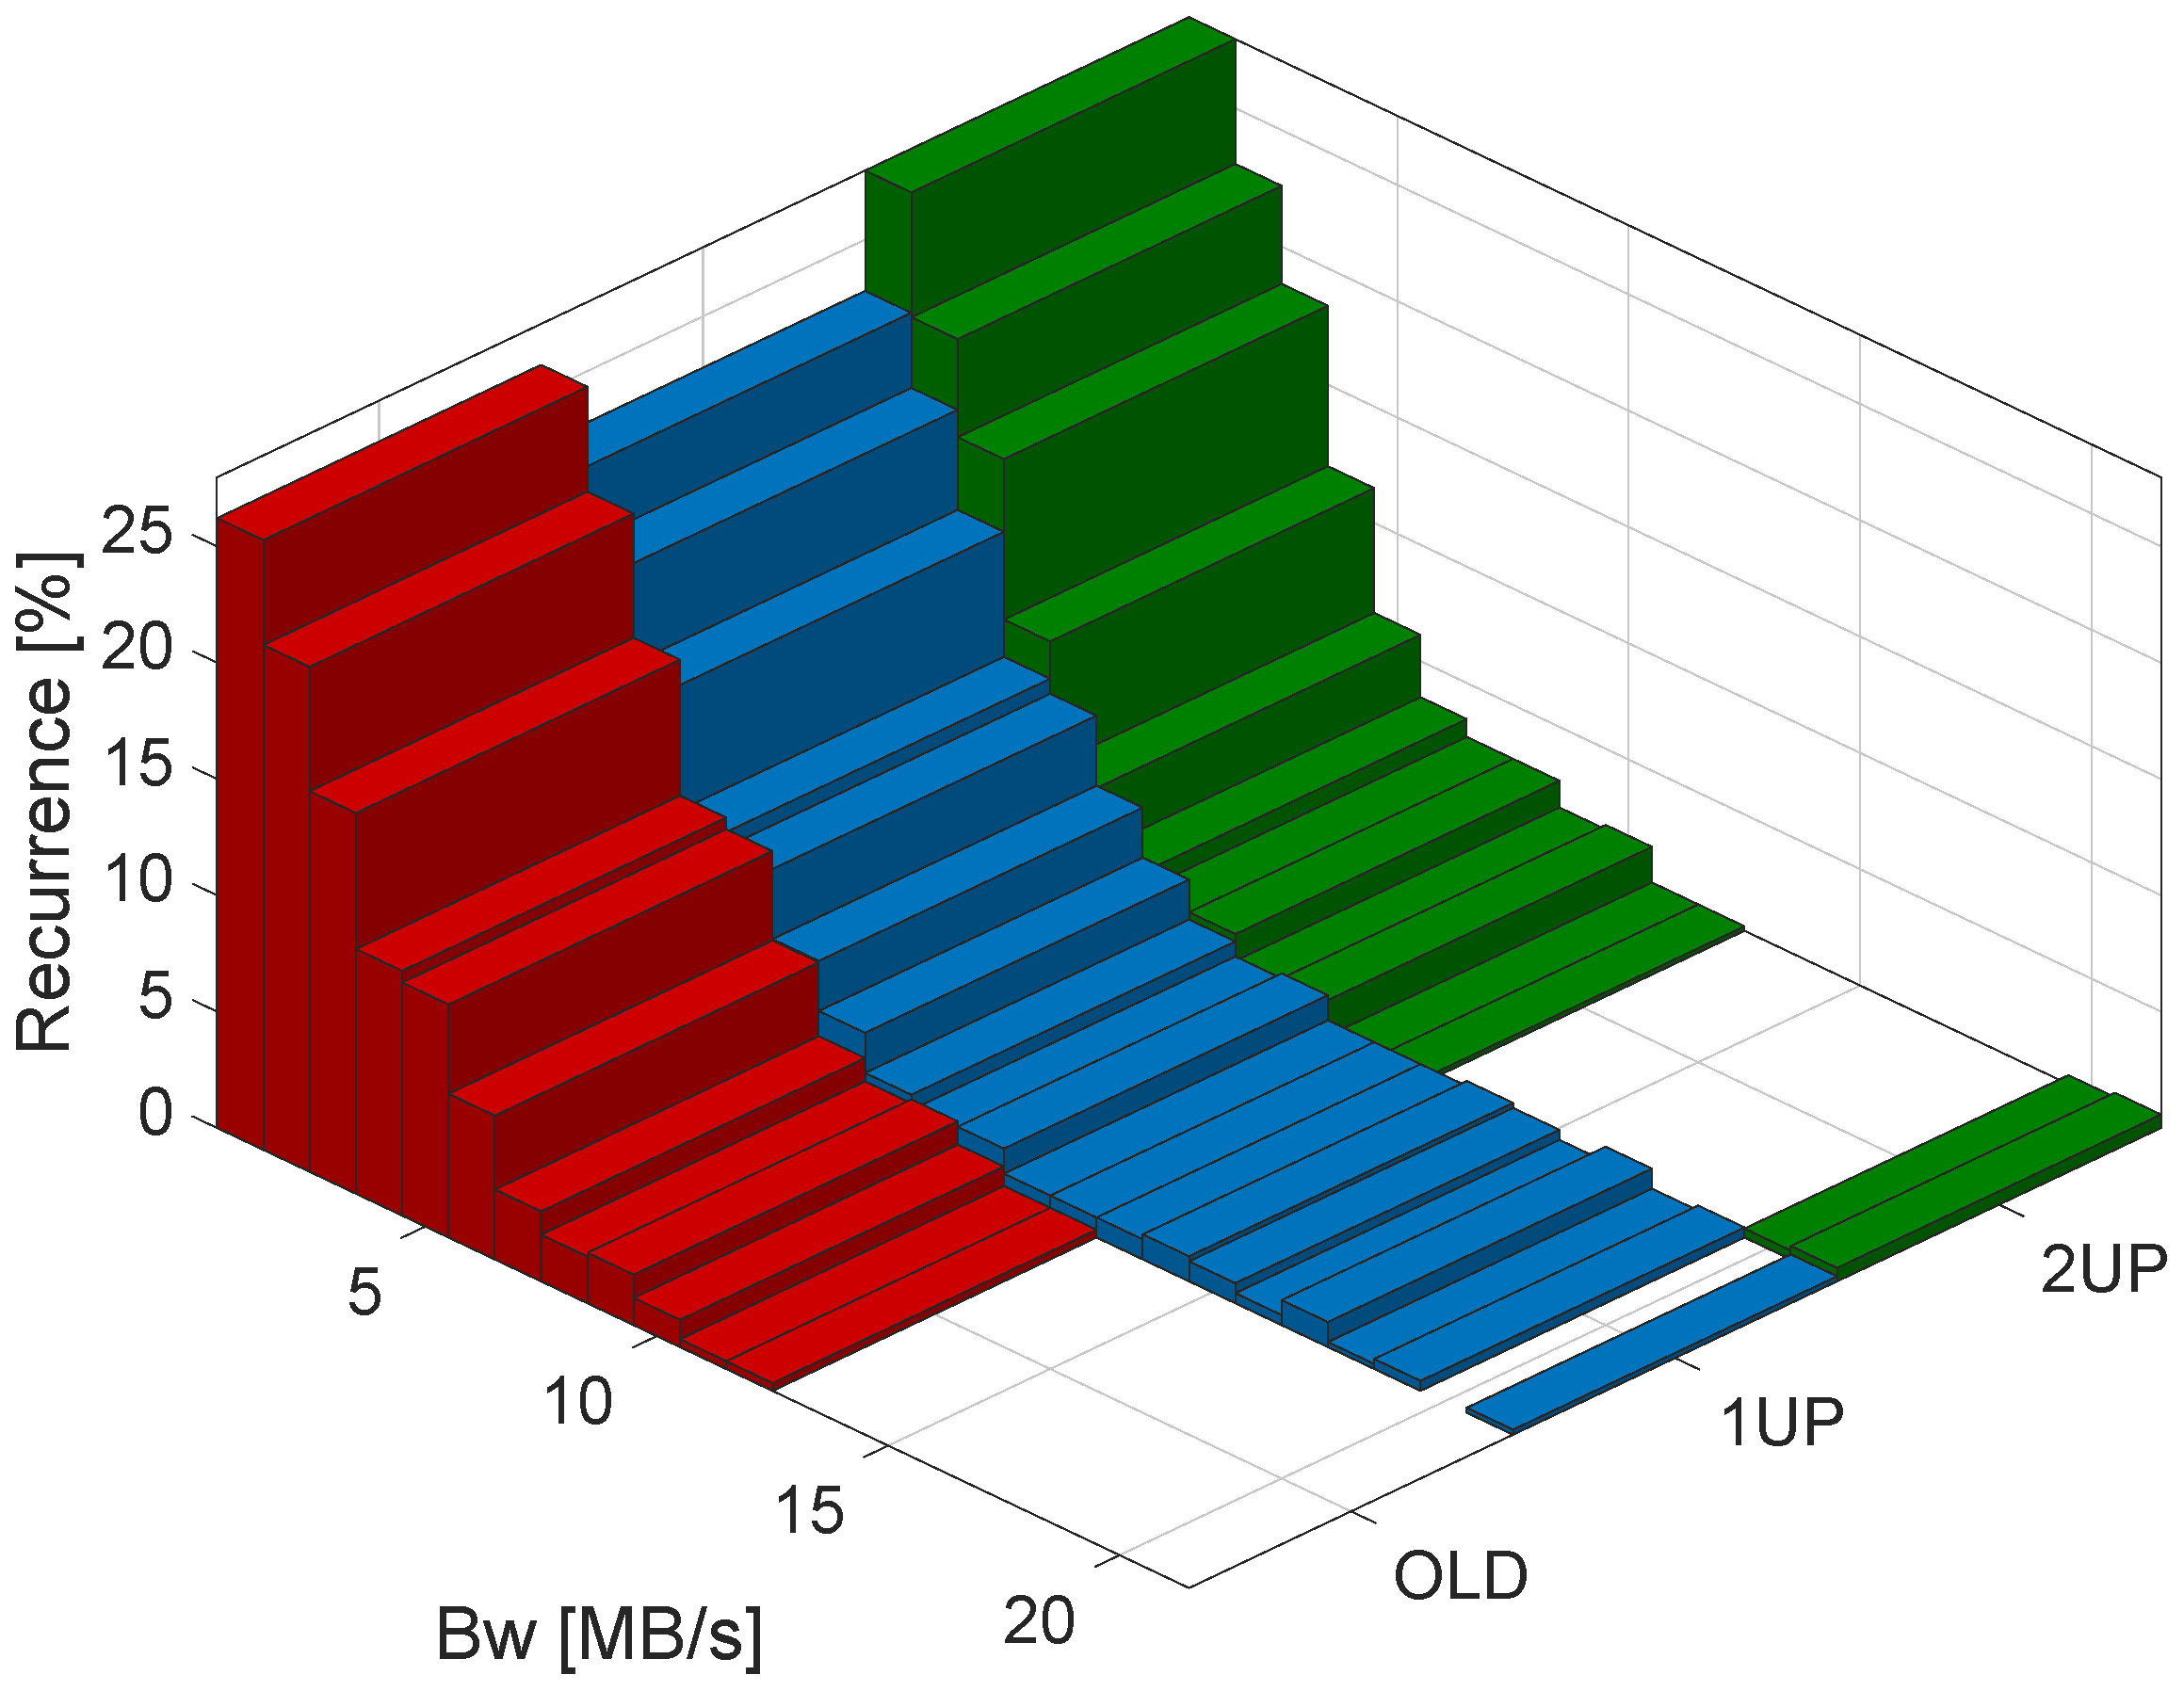
\includegraphics[width=0.7\linewidth]{figure/BW_Pred.eps}}
\caption{Bandwidth saving comparison without (a) and with (b) knowledge of the future disturbances.}
\label{fig:BW}
\end{figure}

Figure \ref{fig:BW} illustrates the bandwidth savings showing the recurrence of the different bandwidth usage during the simulations, respectively without and with knowledge of the future disturbances. Without disturbance forecast we exploited up to $25MB/s$ using the OLD model, while we exploited at most $22MB/s$ and $21MB/s$ respectively for models 1UP and 2UP. Using disturbance forecast, as expected, even less bandwidth is exploited.

\begin{figure}[h!]
\centering
\includegraphics[trim={120 0 120 0},width=0.9\linewidth]{figure/MPCfinal.eps}
\caption{Static controller up to the $400th$, then MPC controller.}
\label{fig:{MPC}}
\end{figure}
%\begin{figure}[h!]
%	\centering
%	\includegraphics[trim={120 0 120 0},width=0.7\linewidth]{figure/banda.eps}
%	\vspace{-0.2cm}
%	\caption{MPC controller: packets sent from the queues (orange), packets lost (red), bandwidth saving (blue).}
%	\vspace{-0.5cm}
%	\label{fig:{BWsave}}
%\end{figure}

We conclude this thesis by quantifying the gap between priority queueing control performance of MPC, obtained solving Problem \ref{pbMPC} and based on our RF predictive model, with the static control policy adopted by service provider networks in \cite{Notiziario}. Figure \ref{fig:{MPC}} highlights the dramatic improvement of MPC with respect to static control: the red line shows the incoming traffic, the blue line shows the sum of the packets sent from the queues, and their difference represents packet losses. Until the $400th$ static control has been implemented as in \cite{Notiziario}, generating many packet losses due to queues saturation. From that sample to the end of our experimentation we implemented MPC using our RF-based model, drastically reducing packet losses: quantitatively, after $700$ sampling periods the cumulative number of dropped packets with the static policy is about $5.5\cdot10^8$ versus $6.6\cdot10^6$ with MPC, with a decrease of $5.434\cdot10^8$ lost packets ($-88 \%$).
%Figure \ref{fig:{BWsave}} shows the amount of bandwidth that our method leaves unused at each time sample (blue line): during the simulation period we were able to save an average $3 MB/s$ with respect to static control, with peaks of more than $20 MB/s$, that can be of course allocated to improve the quality of other services.
We remark that, even thought the improvement of MPC with respect to static control is not surprising, much better performance can be obtained in real networks just collecting historical data and applying a controller that can be directly implemented using the accurate models of our identification algorithms and Quadratic Programming standard solvers.

\chapter{Modeling Real Networks}
\section{Traffic predictive model validation on Italian Internet provider network data}

{In addition to the validation of our predictive models of the incoming traffic over the Mininet environment, the accuracy has been also tested on data measured from a real network device (Ubiquiti EP-16) of an Italian internet internet provider (Sonicatel S.r.l.). Data collection has been performed using the software Cacti \cite{Cacti}.\\
Since this device is part of a running commercial network, some constraints in data collection have forced to only measure the sum of all packets entering and leaving the device, and it has been possible to extract from such traffic only incoming VOIP packets: i.e., it has not been possible to extract packets differentiated for each DSCP. Moreover, it is not currently possible to apply any type of closed-loop control on the network device. For the above 2 reasons the control performance validation in the following sections is not based on this real traffic dataset.\\
About data analysis, 53 days of data measurements have been used for RF training and about 3 days for model validation. Figure \ref{fig:{errorPescara}} shows the prediction on three classes of packets: all packets received, all packets transmitted, VOIP packets received. The plots show that our methodology provides a very accurate prediction even on a real internet service provider network.}
\begin{figure}[h!]
	\centering
	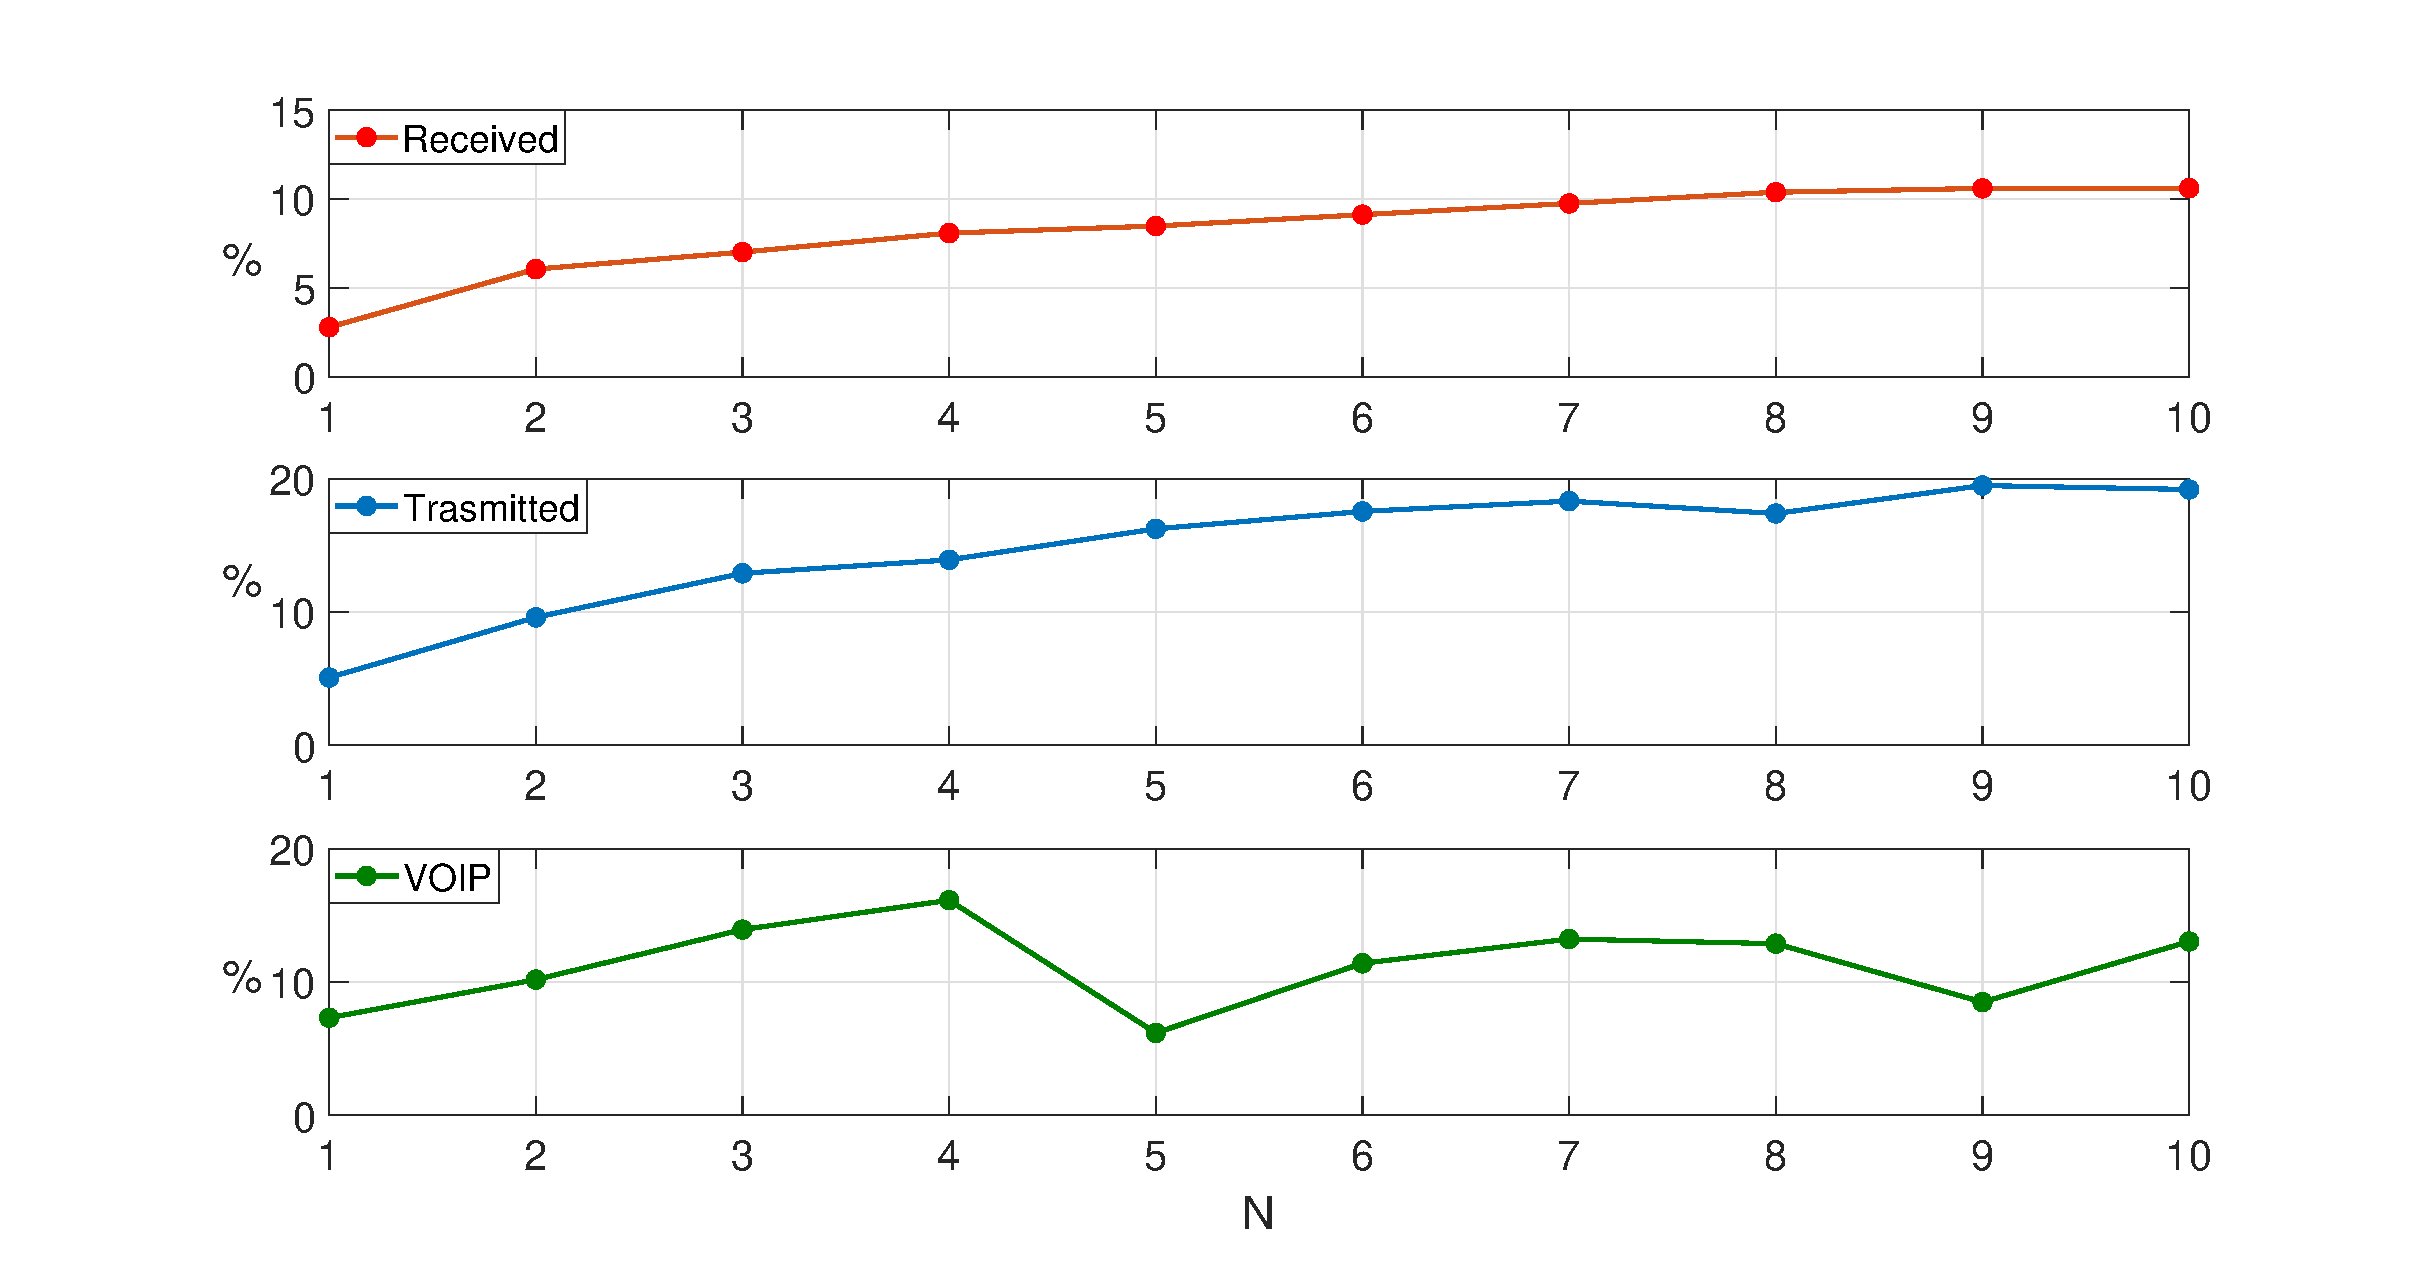
\includegraphics[trim={120 0 120 0}, width=1\linewidth]{figure/Error_PESCARA_DATA.eps}
	\caption{NRMSE of the packets predictive model over a time horizon of $N=10$.}
	\label{fig:{errorPescara}}
\end{figure}

\section{Control performance validation over dedicated hardware network}

\addcontentsline{toc}{chapter}{Conclusion}
\chapter*{Conclusion} 
In this work a new methodology to derive accurate models for priority queueing in Software Defined Networks, in order to enable the application of advanced optimization techniques such as MPC, has been developed and validated over the Mininet network emulator framework and over a dedicated hardware network. The obtained results validate the prediction accuracy both of the incoming traffic and of the input/output behavior of a switch device in a SDN-based network. They also provide promising insights on the potential impact of predictive models combined with MPC in terms of packet losses reduction and bandwidth savings. Furthermore, it has been shown that this method obtains excellent prediction results on data coming from a real network of an Italian internet provider (Sonicatel s.r.l.), proving that the proposed control would be very useful to current communications networks to guarantee the required QoS. In future work it has been planned to validate the proposed controller over real network devices, instead of using Mininet.



%next line adds the Bibliography to the contents page
\addcontentsline{toc}{chapter}{References}
%uncomment next line to change bibliography name to references
\renewcommand{\bibname}{References}
\bibliography{SDN}        %use a bibtex bibliography file refs.bib
\bibliographystyle{elsarticle-num}  %use the plain bibliography style

\addcontentsline{toc}{chapter}{Publications}
\renewcommand{\bibname}{Publications}

\begin{thebibliography}{4}
\bibitem[1]{1} Enrico Reticcioli, Tommaso Campi, Valerio De Santis, An Automated Scanning System for the Acquisition of Non-Uniform Time-Varying Magnetic Fields, IEEE Transactions on Instrumentation and Measurement, 2019

\bibitem[2]{2}Achin Jain, Francesco Smarra, Enrico Reticcioli, Alessandro D'Innocenzo, Manfred Morari, NeurOpt: Neural network based optimization for building energy management and climate control, Learning for Dynamics and Control (L4DC) conference, 2020

\bibitem[3]{3}Enrico Reticcioli, Giovanni Domenico Di Girolamo, Francsco Smarra, Alessio Carmenini, Alessandro D’Innocenzo and Fabio Graziosi, Learning SDN traffic flow accurate models to enable queue bandwidth dynamic optimization, European Conference on Networks and Communications (EuCNC 2020) conference, 2020

\bibitem[4]{4}Enrico Reticcioli, Giovanni Domenico Di Girolamo, Francsco Smarra, Fabio Graziosi and Alessandro D’Innocenzo, Model Identification and Control of Priority Queueing in Software Defined Networks, Submitted to Computer Networks, 2020
\end{thebibliography}
%\bibliographystyle{plain}
%\begin{abstractlong}

\end{abstractlong}      % include the contribution

%Appendix A
\appendix
\lstset{firstnumber=1}
\chapter{Python Codes for Mininet Environment}\label{Py_codes}
\section{datapath\textunderscore monitor\textunderscore TOS.py}\label{datapath_monitor_TOS}
\lstinputlisting[language=Python]{datapath_monitor_TOS.py}
%-------------------------------------------------------------------
\section{main\textunderscore controller\textunderscore TOS.py}\label{main_controller_TOS}
\lstinputlisting[language=Python]{main_controller_TOS.py}
%-------------------------------------------------------------------
\section{Controller\textunderscore commands.py}\label{Controller_commands}
\lstinputlisting[language=Python]{Controller_commands.py}
%-------------------------------------------------------------------
\section{Topology\textunderscore qos\textunderscore TRAFFIC\textunderscore GEN.py}\label{Topology}
\lstinputlisting[language=Python]{Topology_qos_TRAFFIC_GEN.py}
%-------------------------------------------------------------------
\section{ditg.py}\label{ditg}
\lstinputlisting[language=Python]{ditg.py}
%-------------------------------------------------------------------
\section{qos\textunderscore simple\textunderscore switch\textunderscore 13.py}\label{qos_simple_switch_13}
\lstinputlisting[language=Python]{qos_simple_switch_13.py}
%-------------------------------------------------------------------
\section{ofctl\textunderscore rest.py}\label{ofctl_rest}
\lstinputlisting[language=Python]{ofctl_rest.py}
%-------------------------------------------------------------------
\section{rest\textunderscore conf\textunderscore switch.py}\label{rest_conf_switch}
\lstinputlisting[language=Python]{rest_conf_switch.py}
%-------------------------------------------------------------------
\section{rest\textunderscore qos.py}\label{rest_qos}
\lstinputlisting[language=Python]{rest_qos.py}
%-------------------------------------------------------------------

%Appendix B
\lstset{firstnumber=2}
\chapter{Codes For Dedicated Hardware Network Devices}\label{Py_codes_RNT}
\section{Traffic\textunderscore Real\textunderscore Hwd.py}\label{Traffic_Real_Hwd}
\lstinputlisting[language=Python]{RLNT/Traffic_Real_Hwd.py}
%-------------------------------------------------------------------
\section{Start\textunderscore ITGRecv.py}\label{Start_ITGRecv}
\lstinputlisting[language=Python]{RLNT/Start_ITGRecv.py}
%-------------------------------------------------------------------
\section{ditg.py}\label{ditg_RLNT}
\lstinputlisting[language=Python]{RLNT/ditg.py}
%-------------------------------------------------------------------
\section{Set\textunderscore Queue.py}\label{Set_Queue}
\lstinputlisting[language=Python]{RLNT/Set_Queue.py}
%-------------------------------------------------------------------
\section{SendTime.py}\label{SendTime}
\lstinputlisting[language=Python]{RLNT/SendTime.py}
%-------------------------------------------------------------------
\section{ReadTime.ino}\label{ReadTime}
\lstinputlisting[language=Arduino]{RLNT/LetturaSerialePython.ino}
%-------------------------------------------------------------------




\end{document}
